% Options for packages loaded elsewhere
\PassOptionsToPackage{unicode}{hyperref}
\PassOptionsToPackage{hyphens}{url}
\PassOptionsToPackage{dvipsnames,svgnames*,x11names*}{xcolor}
%
\documentclass[
  ngerman,
]{scrbook}
\usepackage{amsmath,amssymb}
\usepackage{lmodern}
\usepackage{ifxetex,ifluatex}
\ifnum 0\ifxetex 1\fi\ifluatex 1\fi=0 % if pdftex
  \usepackage[T1]{fontenc}
  \usepackage[utf8]{inputenc}
  \usepackage{textcomp} % provide euro and other symbols
\else % if luatex or xetex
  \usepackage{unicode-math}
  \defaultfontfeatures{Scale=MatchLowercase}
  \defaultfontfeatures[\rmfamily]{Ligatures=TeX,Scale=1}
\fi
% Use upquote if available, for straight quotes in verbatim environments
\IfFileExists{upquote.sty}{\usepackage{upquote}}{}
\IfFileExists{microtype.sty}{% use microtype if available
  \usepackage[]{microtype}
  \UseMicrotypeSet[protrusion]{basicmath} % disable protrusion for tt fonts
}{}
\makeatletter
\@ifundefined{KOMAClassName}{% if non-KOMA class
  \IfFileExists{parskip.sty}{%
    \usepackage{parskip}
  }{% else
    \setlength{\parindent}{0pt}
    \setlength{\parskip}{6pt plus 2pt minus 1pt}}
}{% if KOMA class
  \KOMAoptions{parskip=half}}
\makeatother
\usepackage{xcolor}
\IfFileExists{xurl.sty}{\usepackage{xurl}}{} % add URL line breaks if available
\IfFileExists{bookmark.sty}{\usepackage{bookmark}}{\usepackage{hyperref}}
\hypersetup{
  pdftitle={A Student's Guide to R},
  pdfauthor={Bianca Krol, Sebastian Sauer, Roger Bons, Oliver Gansser, Matthias Gehrke, Herbert Hollmann, Tanja Kistler, Andreas Kladroba und Thomas Weiß},
  pdflang={de-DE},
  colorlinks=true,
  linkcolor=Maroon,
  filecolor=Maroon,
  citecolor=Blue,
  urlcolor=Blue,
  pdfcreator={LaTeX via pandoc}}
\urlstyle{same} % disable monospaced font for URLs
\usepackage[left=3cm,right=3cm,top=2cm,bottom=2cm]{geometry}
\usepackage{color}
\usepackage{fancyvrb}
\newcommand{\VerbBar}{|}
\newcommand{\VERB}{\Verb[commandchars=\\\{\}]}
\DefineVerbatimEnvironment{Highlighting}{Verbatim}{commandchars=\\\{\}}
% Add ',fontsize=\small' for more characters per line
\usepackage{framed}
\definecolor{shadecolor}{RGB}{248,248,248}
\newenvironment{Shaded}{\begin{snugshade}}{\end{snugshade}}
\newcommand{\AlertTok}[1]{\textcolor[rgb]{0.94,0.16,0.16}{#1}}
\newcommand{\AnnotationTok}[1]{\textcolor[rgb]{0.56,0.35,0.01}{\textbf{\textit{#1}}}}
\newcommand{\AttributeTok}[1]{\textcolor[rgb]{0.77,0.63,0.00}{#1}}
\newcommand{\BaseNTok}[1]{\textcolor[rgb]{0.00,0.00,0.81}{#1}}
\newcommand{\BuiltInTok}[1]{#1}
\newcommand{\CharTok}[1]{\textcolor[rgb]{0.31,0.60,0.02}{#1}}
\newcommand{\CommentTok}[1]{\textcolor[rgb]{0.56,0.35,0.01}{\textit{#1}}}
\newcommand{\CommentVarTok}[1]{\textcolor[rgb]{0.56,0.35,0.01}{\textbf{\textit{#1}}}}
\newcommand{\ConstantTok}[1]{\textcolor[rgb]{0.00,0.00,0.00}{#1}}
\newcommand{\ControlFlowTok}[1]{\textcolor[rgb]{0.13,0.29,0.53}{\textbf{#1}}}
\newcommand{\DataTypeTok}[1]{\textcolor[rgb]{0.13,0.29,0.53}{#1}}
\newcommand{\DecValTok}[1]{\textcolor[rgb]{0.00,0.00,0.81}{#1}}
\newcommand{\DocumentationTok}[1]{\textcolor[rgb]{0.56,0.35,0.01}{\textbf{\textit{#1}}}}
\newcommand{\ErrorTok}[1]{\textcolor[rgb]{0.64,0.00,0.00}{\textbf{#1}}}
\newcommand{\ExtensionTok}[1]{#1}
\newcommand{\FloatTok}[1]{\textcolor[rgb]{0.00,0.00,0.81}{#1}}
\newcommand{\FunctionTok}[1]{\textcolor[rgb]{0.00,0.00,0.00}{#1}}
\newcommand{\ImportTok}[1]{#1}
\newcommand{\InformationTok}[1]{\textcolor[rgb]{0.56,0.35,0.01}{\textbf{\textit{#1}}}}
\newcommand{\KeywordTok}[1]{\textcolor[rgb]{0.13,0.29,0.53}{\textbf{#1}}}
\newcommand{\NormalTok}[1]{#1}
\newcommand{\OperatorTok}[1]{\textcolor[rgb]{0.81,0.36,0.00}{\textbf{#1}}}
\newcommand{\OtherTok}[1]{\textcolor[rgb]{0.56,0.35,0.01}{#1}}
\newcommand{\PreprocessorTok}[1]{\textcolor[rgb]{0.56,0.35,0.01}{\textit{#1}}}
\newcommand{\RegionMarkerTok}[1]{#1}
\newcommand{\SpecialCharTok}[1]{\textcolor[rgb]{0.00,0.00,0.00}{#1}}
\newcommand{\SpecialStringTok}[1]{\textcolor[rgb]{0.31,0.60,0.02}{#1}}
\newcommand{\StringTok}[1]{\textcolor[rgb]{0.31,0.60,0.02}{#1}}
\newcommand{\VariableTok}[1]{\textcolor[rgb]{0.00,0.00,0.00}{#1}}
\newcommand{\VerbatimStringTok}[1]{\textcolor[rgb]{0.31,0.60,0.02}{#1}}
\newcommand{\WarningTok}[1]{\textcolor[rgb]{0.56,0.35,0.01}{\textbf{\textit{#1}}}}
\usepackage{longtable,booktabs,array}
\usepackage{calc} % for calculating minipage widths
% Correct order of tables after \paragraph or \subparagraph
\usepackage{etoolbox}
\makeatletter
\patchcmd\longtable{\par}{\if@noskipsec\mbox{}\fi\par}{}{}
\makeatother
% Allow footnotes in longtable head/foot
\IfFileExists{footnotehyper.sty}{\usepackage{footnotehyper}}{\usepackage{footnote}}
\makesavenoteenv{longtable}
\usepackage{graphicx}
\makeatletter
\def\maxwidth{\ifdim\Gin@nat@width>\linewidth\linewidth\else\Gin@nat@width\fi}
\def\maxheight{\ifdim\Gin@nat@height>\textheight\textheight\else\Gin@nat@height\fi}
\makeatother
% Scale images if necessary, so that they will not overflow the page
% margins by default, and it is still possible to overwrite the defaults
% using explicit options in \includegraphics[width, height, ...]{}
\setkeys{Gin}{width=\maxwidth,height=\maxheight,keepaspectratio}
% Set default figure placement to htbp
\makeatletter
\def\fps@figure{htbp}
\makeatother
\setlength{\emergencystretch}{3em} % prevent overfull lines
\providecommand{\tightlist}{%
  \setlength{\itemsep}{0pt}\setlength{\parskip}{0pt}}
\setcounter{secnumdepth}{5}
\usepackage{booktabs}
\usepackage{fontawesome}
\usepackage{xcolor}

\usepackage{tcolorbox}
\usepackage{color}
\usepackage{framed}
\setlength{\fboxsep}{.7em}

\usepackage{amsthm}
\usepackage{csquotes}  % ses 2018-01-04
\usepackage{xspace}
\usepackage{graphicx}
\usepackage{FOMTitle}
\usepackage{setspace}

\makeatletter
\def\thm@space@setup{%
  \thm@preskip=4pt plus 2pt minus 4pt
  \thm@postskip=\thm@preskip
}
\makeatother


\definecolor{dark-fom-green}{HTML}{00998a}
\definecolor{fom-green}{HTML}{4cb7ad}
\definecolor{FOMSubTitelColor}{HTML}{32373D}
\definecolor{light-grey}{HTML}{fdfdfd}

\newtcolorbox{blackbox}{
  colback=light-grey,
  colframe=dark-fom-green,
  coltext=black,
  left=1pt,
  arc=2pt}

\newenvironment{infobox}[1]
  {
  \begin{itemize}
  \renewcommand{\labelitemi}{
    \raisebox{1.8\height}[0pt][0pt]{
       {\setkeys{Gin}{width=7em,keepaspectratio}
        {\Large \textcolor{dark-fom-green}\faLightbulbO}}
        }
  }
  %\setlength{\fboxsep}{1em}
  \begin{blackbox}
        % \medskip
        \bgroup\color{dark-fom-green}
          {\textbf{Info}}
        \egroup
        % \medskip
  \item
  }
  {
  \end{blackbox}
  \end{itemize}
  }
  
\newenvironment{tiefereinsteigen}[1]
  {
  \begin{itemize}
  \renewcommand{\labelitemi}{
    \raisebox{2.6\height}[0pt][0pt]{
      {\setkeys{Gin}{width=7em,keepaspectratio}
        {\normalsize \textcolor{dark-fom-green}\faSearch}}
        }
  }
  %\setlength{\fboxsep}{1em}
  \begin{blackbox}
        %\medskip
         \bgroup\color{dark-fom-green}
          {\textbf{Tiefer einsteigen}}
        \egroup
        %\medskip
  \item
  }
  {
  \end{blackbox}
  \end{itemize}
  }
  
\newenvironment{hinweis}[1]
  {
  \begin{itemize}
  \renewcommand{\labelitemi}{
    \raisebox{1.8\height}[0pt][0pt]{
      {\setkeys{Gin}{width=7em,keepaspectratio}
        {\Large \textcolor{dark-fom-green}\faHandORight}}
        }
  }
  %\setlength{\fboxsep}{1em}
  \begin{blackbox}
        %\medskip
        \bgroup\color{dark-fom-green}
          {\textbf{Hinweis}}
        \egroup
        %\medskip
  \item
  }
  {
  \end{blackbox}
  \end{itemize}
  }

\newenvironment{achtung}[1]
  {
  \begin{itemize}
  \renewcommand{\labelitemi}{
    \raisebox{1.8\height}[0pt][0pt]{
      {\setkeys{Gin}{width=7em,keepaspectratio}
        {\Large \textcolor{dark-fom-green}\faExclamationCircle}}
        }
  }
  %\setlength{\fboxsep}{1em}
  \begin{blackbox}
        %\medskip
        \bgroup\color{dark-fom-green}
          {\textbf{Achtung!}}
        \egroup
        %\medskip
  \item
  }
  {
  \end{blackbox}
  \end{itemize}
  }
  
\newenvironment{note}[1]
  {
  \begin{itemize}
  \renewcommand{\labelitemi}{
    \raisebox{-.01\height}[0pt][0pt]{
      {\setkeys{Gin}{width=7em,keepaspectratio}
        {\normalsize \textcolor{dark-fom-green}\faHashtag}}
        }
  }
  %\setlength{\fboxsep}{1em}
  \begin{blackbox}
   \item
    }
    {
  \end{blackbox}
  \end{itemize}
  }

\newenvironment{aufgabe}[1]
  {
  \begin{itemize}
  \renewcommand{\labelitemi}{
    \raisebox{1.8\height}[0pt][0pt]{
      {\setkeys{Gin}{width=7em,keepaspectratio}
        {\Large \textcolor{dark-fom-green}\faFileCodeO}}
        }
  }
  %\setlength{\fboxsep}{1em}
  \begin{blackbox}
        %\medskip
        \bgroup\color{dark-fom-green}
          {\textbf{Aufgabe!}}
        \egroup
        %\medskip
   \item
    }
    {
  \end{blackbox}
  \end{itemize}
  }
\usepackage{booktabs}
\usepackage{longtable}
\usepackage{array}
\usepackage{multirow}
\usepackage{wrapfig}
\usepackage{float}
\usepackage{colortbl}
\usepackage{pdflscape}
\usepackage{tabu}
\usepackage{threeparttable}
\usepackage{threeparttablex}
\usepackage[normalem]{ulem}
\usepackage{makecell}
\usepackage{xcolor}
\ifxetex
  % Load polyglossia as late as possible: uses bidi with RTL langages (e.g. Hebrew, Arabic)
  \usepackage{polyglossia}
  \setmainlanguage[]{german}
\else
  \usepackage[main=ngerman]{babel}
% get rid of language-specific shorthands (see #6817):
\let\LanguageShortHands\languageshorthands
\def\languageshorthands#1{}
\fi
\ifluatex
  \usepackage{selnolig}  % disable illegal ligatures
\fi
\usepackage[]{biblatex}
\addbibresource{bib/book.bib}
\addbibresource{bib/packages.bib}
\addbibresource{bib/article.bib}

\title{A Student's Guide to R}
\usepackage{etoolbox}
\makeatletter
\providecommand{\subtitle}[1]{% add subtitle to \maketitle
  \apptocmd{\@title}{\par {\large #1 \par}}{}{}
}
\makeatother
\subtitle{Übersetzung des englischen Originals}
\author{Bianca Krol, Sebastian Sauer, Roger Bons, Oliver Gansser, Matthias Gehrke, Herbert Hollmann, Tanja Kistler, Andreas Kladroba und Thomas Weiß}
\date{2021-07-09}

\begin{document}
\maketitle

{
\hypersetup{linkcolor=}
\setcounter{tocdepth}{1}
\tableofcontents
}
\hypertarget{vorwort}{%
\chapter*{Vorwort}\label{vorwort}}
\addcontentsline{toc}{chapter}{Vorwort}

In 2016 hat die FOM Hochschule für Oekonomie \& Management sich auf den Weg gemacht, in der Methodenausbildung die Kompetenz der Data Literacy zu fokussieren. In den zurückliegenden Semestern wurde die Ausbildung daher in Anlehnung an die \href{https://www.amstat.org/asa/files/pdfs/GAISE/GaiseCollege_Full.pdf}{GAISE}(Guidelines for Assessment and Instruction in Statistics Education)-Empfehlungen modernisiert. 2019 wurde die FOM aufgrund dieses Ausbildungskonzeptes in das \href{https://www.stifterverband.org/data-literacy-education}{Data Literacy Education Netzwerk des Stifterverbandes} aufgenommen und zu Beginn dieses Jahres hat die FOM die \href{https://www.stifterverband.org/charta-data-literacy}{Data-Literacy-Charta} unterschrieben, in der Folgendes zu finden ist: ``Data Literacy umfasst die Datenkompetenzen, die für alle Menschen in einer durch Digitalisierung geprägten Welt wichtig sind. Sie ist unverzichtbarer Bestandteil der Allgemeinbildung.''

Diesem Anspruch versuchen wir im Rahmen unserer Methodenausbildung gerecht zu werden. Um daten-literat zu werden, liegt der Fokus unserer Ausbildung auf dem konzeptionellen Verstehen, der Betonung des gesamten Analyseprozesses (von der Frage bis zur vorläufigen Antwort), der Befähigung von Studierenden zur verantwortungsvollen Nutzung von Daten im beruflichen und akademischen Kontext sowie der Sensibilisierung von Studierenden für reproduzierbare empirische Analysen. Dazu setzen wir in der Lehre auf Unterstützung durch R, RStudio und mosaic.

Das Paket mosaic hilft in der Ausbildung, da es den R Code vereinheitlicht und die Grundlage für ein \emph{Denken mit Daten}\footnote{\href{https://journal.r-project.org/archive/2017/RJ-2017-024/index.html}{Pruim, R., Kaplan, D.T. und Horton, N.J. (2017): The mosaic Package: Helping Students to `Think with Data' Using R. The R Journal, 9(1), 77-10}} bildet. Es findet sich unzählige Literatur zu R und RStudio. Dazu gehört auch \href{https://github.com/ProjectMOSAIC/LittleBooks/raw/master/StudentGuide/MOSAIC-StudentGuide.pdf}{A Student's Guide to R} von Nicholas J. Horton, Randall Pruim und Daniel T. Kaplan, der eine gute Einstiegshilfe für Studierende ist, um erste Schritte in der Datenanalyse mit R zu machen.

Da die englische Sprache ein Hemmnis bei der Einarbeitung in eine neue Materie, wie die der Datenanalyse, sein kann, haben wir uns die Erlaubnis eingeholt, den Student's Guide auf Deutsch zu übersetzen. Vielen Dank dafür an Nicholas Horton!

Ein solches Projekt kann nur gelingen, wenn sich engagierte Kolleginnen und Kollegen mit einbringen. Daher danken wir an dieser Stelle Roger Bons, Oliver Gansser, Matthias Gehrke, Herbert Hollmann, Tanja Kistler, Andreas Kladroba und Thomas Weiß, die sich der Übersetzung von Kapiteln angenommen haben. Ein besonderer Dank geht an Sebastian Sauer, der ebenfalls Kapitel übersetzt hat und der das Projekt maßgeblich mit angestoßen hat. Ebenso möchten wir uns bei Tabea Griesenbeck, wissenschaftliche Mitarbeiterin am ifes, bedanken, die die Organisation, das Layout und die Korrekturen übernommen hat.

Wir hoffen, dass die deutschsprachige Version des Student's Guide to R unseren Studierenden ab dem Wintersemester 2021 eine weitere, zielführende Hilfestellung ist.

Prof.~Dr.~Bianca Krol\\
Dekanin \textbar{} Schlüsselkompetenzen \& Methoden
Direktorin \textbar{} ifes Institut für Empirie \& Statistik

Prof.~Dr.~habil. Andrea Schankin
(hier fehlt noch der Untertitel und es wäre toll, wenn wir die Namen nebeneinander setzen könnten)

Wo kommt das hier her?: Dieses Buch baut technnisch auf \emph{knitr} \autocite{xie2015}, \emph{rmarkdown} \autocite{R-rmarkdown}, R \autocite{R-base} und vielen weiteren Open-Source-Anwendungen. Details sind im Kapitel \ref{hinweise} hinterlegt. Lorem Ipsum.

\hypertarget{einleitung}{%
\chapter{Einleitung}\label{einleitung}}

Dieses Referenzbuch beinhaltet einen Überblick über die Befehle und Funktionen, die zur Bearbeitung von Daten im Rahmen von Statistikkursen für Einsteiger und Fortgeschrittene benötigt werden. Ziel ist es, eine Ergänzung zu den Büchern \emph{Start Teaching with R} \autocite{TeachingR} und \emph{Start Modeling with R} \autocite{ModelingR} zur Verfügung zu stellen.

In den meisten der hier verwendeten Beispiele werden Daten der HELP-Studie (Health Evaluation and Linkage to Primary Care) verwendet: Ein randomisiertes klinisches Experiment mit einer neuen Vorgehensweise, die Risikopatienten mit Primärversorgern zusammenbringen soll. Ausführlichere Informationen zu dem Datensatz sind in Kapitel \ref{HELPstudie} enthalten.

Die Themenauswahl und -reihenfolge ist von Lehrbuch zu Lehrbuch sehr unterschiedlich gestaltet, weswegen die Gliederung dieses Buches anhand der Art der Daten, die analysiert werden sollen, vorgenommen wurde. Damit soll das Nachschlagen und Auffinden benötigter Informationen vereinfacht werden. Gewisse Fähigkeiten im Bereich des Datenmanagements sind für Studierende essentiell \autocite{ChanceInClass}.

In Kapitel \ref{datenmanagement} gibt es eine Einführung zu den wichtigsten Kernbegriffen.

Dieses Werk baut auf die Initiativen des MOSAIC Projektes \url{http://www.mosaic-web.org} auf: Ein durch die amerikanische National Science Foundation (NSF) gefördertes Programm, um den Unterricht von Statistik, Mathematik, Naturwissenschaften und Informatik im Grundstudium zu fördern. Wir werden insbesondere das Paket \texttt{mosaic}, das erstellt wurde, um den Einsatz von \textsf{R} in statistischen Kursen zu vereinfachen, und das Paket \texttt{mosaicData}, welches eine Reihe von Datensätzen enthält, einsetzen. Das Paket \texttt{ggformula} bietet hierbei unter Benutzung der \texttt{mosaic}-Syntax Unterstützung für qualitätsvolle Grafiken. Eine Beschreibung des MOSAIC Ansatzes für die Lehre von Statistik und Datenwissenschaft ist verfügbar über \url{https://journal.r-project.org/archive/2017/RJ-2017-024}. Eine kurze Zusammenfassung der \textsf{R} Befehle, die für die Lehre einführender Statistik essentiell ist, steht in der \texttt{vignette} des Paketes \texttt{mosaic} zur Verfügung:
\url{https://cran.r-project.org/web/packages/mosaic}.

Auch weitere Ressourcen des MOSAIC Projektes können nützlich sein, zum Beispiel eine kommentierte Sammlung von Beispielen aus verschiedenen Lehrbüchern (vgl. \url{https://cran.r-project.org/web/packages/mosaic/vignettes/mosaic-resources.html}).

Um ein Paket in \textsf{R} nutzen zu können, muss es zuerst (einmalig) installiert werden und in jeder neuen Session geladen werden. Das Paket \texttt{mosaic} kann mit folgendem Befehl installiert werden:

\begin{Shaded}
\begin{Highlighting}[]
\FunctionTok{install.packages}\NormalTok{(}\StringTok{"mosaic"}\NormalTok{)        }\CommentTok{\# Beachten Sie die Anführungszeichen}
\end{Highlighting}
\end{Shaded}

\begin{note}{note}
\textsf{RStudio} bietet u. a. auch einen Reiter zur Paketinstallation im Panel rechts unten an.

\end{note}

Das \texttt{\#} Zeichen stellt einen Kommentar in R dar und klammert den restlichen Text bis zum Ende der Zeile aus.

Nachdem das Paket einmalig installiert wurde, kann es zur Verwendung der enthaltenen Funktionen über folgenden Befehl geladen werden:

\begin{Shaded}
\begin{Highlighting}[]
\FunctionTok{library}\NormalTok{(mosaic)}
\end{Highlighting}
\end{Shaded}

\textsf{R Markdown} bietet eine einfache markup Sprache, welche die Ergebnisse in PDF, Word oder HTML übersetzt. Das ermöglicht es, Analysen mit einem Workflow zu versehen, der Reproduzierbarkeit sicherstellt und Kopierfehler vermeidet.

\begin{infobox}{infobox}
Das \textsf{knitr/LATEX} System erlaubt dem erfahrenen Nutzer \textsf{R} und \textsf{LaTeX} im selben Dokument zu verknüpfen. Die Belohnung dafür dieses kompliziertere System zu erlernen ist eine viel feinere Kontrolle über das Ausgabeformat. \textsf{R Markdown} ist jedoch deutlich einfacher zu erlernen und eignet sich auch für fachliche Arbeiten.

\end{infobox}

\begin{hinweis}{hinweise}
Um \textsf{Markdown} oder \textsf{knitr/LATEX} nutzen zu können, muss das Paket \texttt{markdown} installiert sein.

\end{hinweis}

Die Einführung in \textsf{R Markdown} erfolgt typischerweise zu Beginn des Kurses, begleitet von der Aufforderung dies von vornherein für Seminar- und Hausarbeiten etc. zu nutzen \autocite{baumer2014r}.

\hypertarget{RStudio}{%
\chapter{Los geht's mit RStudio}\label{RStudio}}

\textsf{RStudio} ist eine integrierte Entwicklerumgebung (\emph{integrated development environment} - IDE) für \textsf{R}, die gegenüber anderen eine alternative Schnittstelle zu \textsf{R} mit mehreren Vorteilen bietet:

\begin{hinweis}{hinweis}
Es gibt eine Reihe an Einführungsvideos unter \url{https://nhorton.people.amherst.edu/rstudio}.

\end{hinweis}

\begin{itemize}
\tightlist
\item
  \textsf{RStudio} läuft auf Mac-, PC-, und Linux-Rechnern und bietet eine vereinfachte Schnittstelle, die vom Aussehen und in der Handhabung auf allen ähnlich ist. Die Standardschnittstellen für \textsf{R} sind ziemlich unterschiedlich auf den verschiedenen Plattformen. Das kann verwirren oder ablenken und zu höherem Unterstützungsaufwand führen.
\item
  \textsf{RStudio} kann in einem Webbrowser ausgeführt werden. Zusätzlich zu eigenständigen Desktop-Versionen oder \textsf{RStudio.cloud} kann \textsf{RStudio} als eine Server-Anwendung installiert werden, die über das Internet zugreifbar ist. Die Web-Schnittstelle ist fast identisch zu der Desktopversion. Wie bei anderen Web-Services auch, melden Nutzer sich an, um Zugriff zu ihrem Konto zu erlangen. Nach Abmeldung und späterer Neuanmeldung, wird die letzte Session wiederhergestellt und Sie können an der Stelle mit ihrer Analyse weiter machen, wo Sie verblieben waren, auch wenn Sie sich auf einem anderen Rechner anmelden. Mit einer etwas fortgeschrittenen Einrichtung können Dozierende die History der \textsf{R}-Session in ihrem Klassenraum speichern und Studierende können diese History-Datei in ihre eigene Umgebung laden.
\end{itemize}

\begin{achtung}{achtung}
Die Desktop- und Server-Versionen von \textsf{RStudio} sind so ähnlich, dass Sie besonders aufpassen müssen, wenn Sie beide gleichzeitig nutzen, um sicher zu gehen, dass Sie in der richtigen Version arbeiten.

\end{achtung}

\begin{note}{note}
Die Verwendung von \textsf{RStudio} in einem Browser ist wie Facebook für Statistik. Jedes Mal, wenn Anwender sich erneut anmelden, wird die vorherige Session wiederhergestellt und sie können weitermachen, wo sie zuletzt aufgehört haben. Nutzer können sich von jedem Gerät mit Internetzugriff anmelden.

\end{note}

\begin{itemize}
\tightlist
\item
  \textsf{RStudio} ist ein Tool, das die Erstellung reproduzierbarer Forschung unterstützt. Es vereinfacht Text, statistische Analysen (\textsf{R}-Code und \textsf{R}-Output) und grafische Abbildungen zusammen im gleichen Dokument zu vereinen. Das \textsf{R Markdown}-System bietet eine einfache Markup Sprache und fügt die Ergebnisse in HTML zusammen. Das \textsc{knitr/LaTeX}-System versetzt Nutzer in die Lage auch \textsf{R} und \textsf{LaTeX} in dasselbe Dokument zu integrieren. Die Belohnung für das Erlernen dieses komplizierteren Systems ist eine deutlich präzisere Steuerung des Output-Formates. Abhängig von der Niveaustufe des Kurses können Sie eins dieser beiden Systeme für Hausarbeiten und Projekte verwenden.
\end{itemize}

\begin{hinweis}{hinweis}
Um Markdown oder \textsc{knitr/LaTeX} zu verwenden, muss das Paket \texttt{knitr} auf dem System installiert sein.

\end{hinweis}

\begin{itemize}
\tightlist
\item
  \textsf{RStudio} bietet eine integrierte Unterstützung für das Bearbeiten und Ausführen von \textsf{R}-Code und Dokumenten.
\item
  \textsf{RStudio} bietet einige nützliche Funktionalitäten über eine grafische Nutzeroberfläche (Graphical User Interface oder GUI). \textsf{RStudio} ist nicht ein GUI für \textsf{R}, aber es bietet ein GUI, das Themen wie die Installation und Verwaltung von Paketen, die Steuerung, Speicherung und das Laden von Umgebungen, das Importieren und Exportieren von Daten sowie den Zugriff auf und Export von Abbildungen, Dateien und Dokumentationen vereinfacht.
\item
  \textsf{RStudio} bietet Zugriff auf das Paket \texttt{manipulate}. Das Paket \texttt{manipulate} bietet eine Möglichkeit, einfach und schnell interaktive grafische Anwendungen zu erstellen.
\end{itemize}

Obwohl man sicherlich \textsf{R} ohne die Verwendung von \textsf{RStudio} nutzen kann, vereinfacht \textsf{RStudio} viele Dinge und wir empfehlen den Einsatz von \textsf{RStudio} stark. Außerdem erwarten wir in Zukunft noch weitere nützliche Funktionalitäten, da \textsf{RStudio} stetig weiterentwickelt wird.

Wir verwenden in erster Linie eine Online-Version von \textsf{RStudio}. Die Anwendung über den Browser hat den Vorteil, dass Sie nichts installieren oder konfigurieren müssen. Einfach anmelden und Sie können loslegen. Außerdem \glqq merkt\grqq  \textsf{ RStudio} sich, was Sie machen und Sie können da weitermachen, wo Sie aufgehört haben, jedesmal wenn Sie sich anmelden (auch auf einem anderen Rechner). Das ist \glqq\textsf{R} in the cloud\grqq und funktioniert ähnlich wie GoogleDocs oder Facebook für \textsf{R}.

\begin{hinweis}
\textsf{R} kann von \url{http://cran.r-project.org/} heruntergeladen und lokal installiert werden. Das Herunterladen und die Installation sind i. ~A. unkompliziert für Mac-, PC-, oder Linux-Systeme. \textsf{RStudio} ist über \url{http://www.rstudio.org/} verfügbar.

\end{hinweis}

\hypertarget{mit-einem-rstudio-server-verbinden}{%
\section{Mit einem RStudio-Server verbinden}\label{mit-einem-rstudio-server-verbinden}}

\textsf{RStudio} Server wurden an Hochschulen eingerichtet, um cloud-basierte Berechnungen zu ermöglichen.

\begin{note}{note}
\textsf{RStudio} Server wurden schon an vielen Institutionen installiert. Nähere Informationen zu (gebührenfreien) akademischen Lizenzen für \textsf{RStudio} Server Pro und Installationsanweisungen sind über \url{http://www.rstudio.com/resources/faqs} unter dem \textsc{Academic} Reiter verfügbar.
Der \textsf{RStudio} Server funktioniert mit dem Internet Explorer allerdings nicht sehr zuverlässig.

\end{note}

Sobald Sie mit dem Server verbunden sind, sollten Sie ein Anmeldefenster sehen:

\begin{center}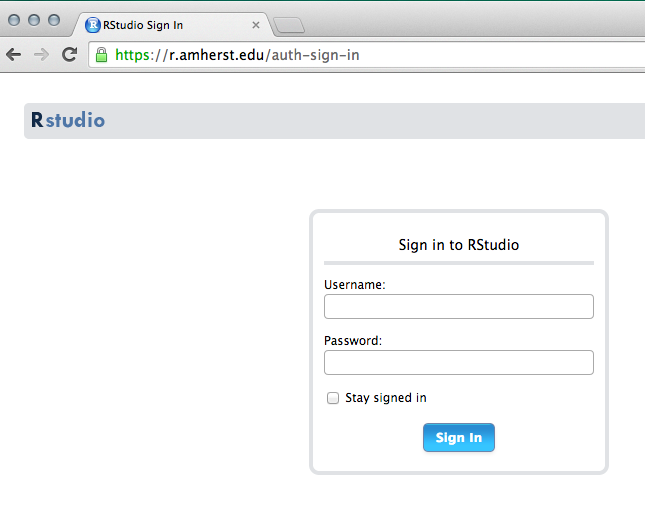
\includegraphics[width=0.5\linewidth]{images/rstudio-login} \end{center}

\newpage

Wenn Sie sich angemeldet haben, sollten Sie die \texttt{RStudio} Schnittstelle sehen:

\begin{center}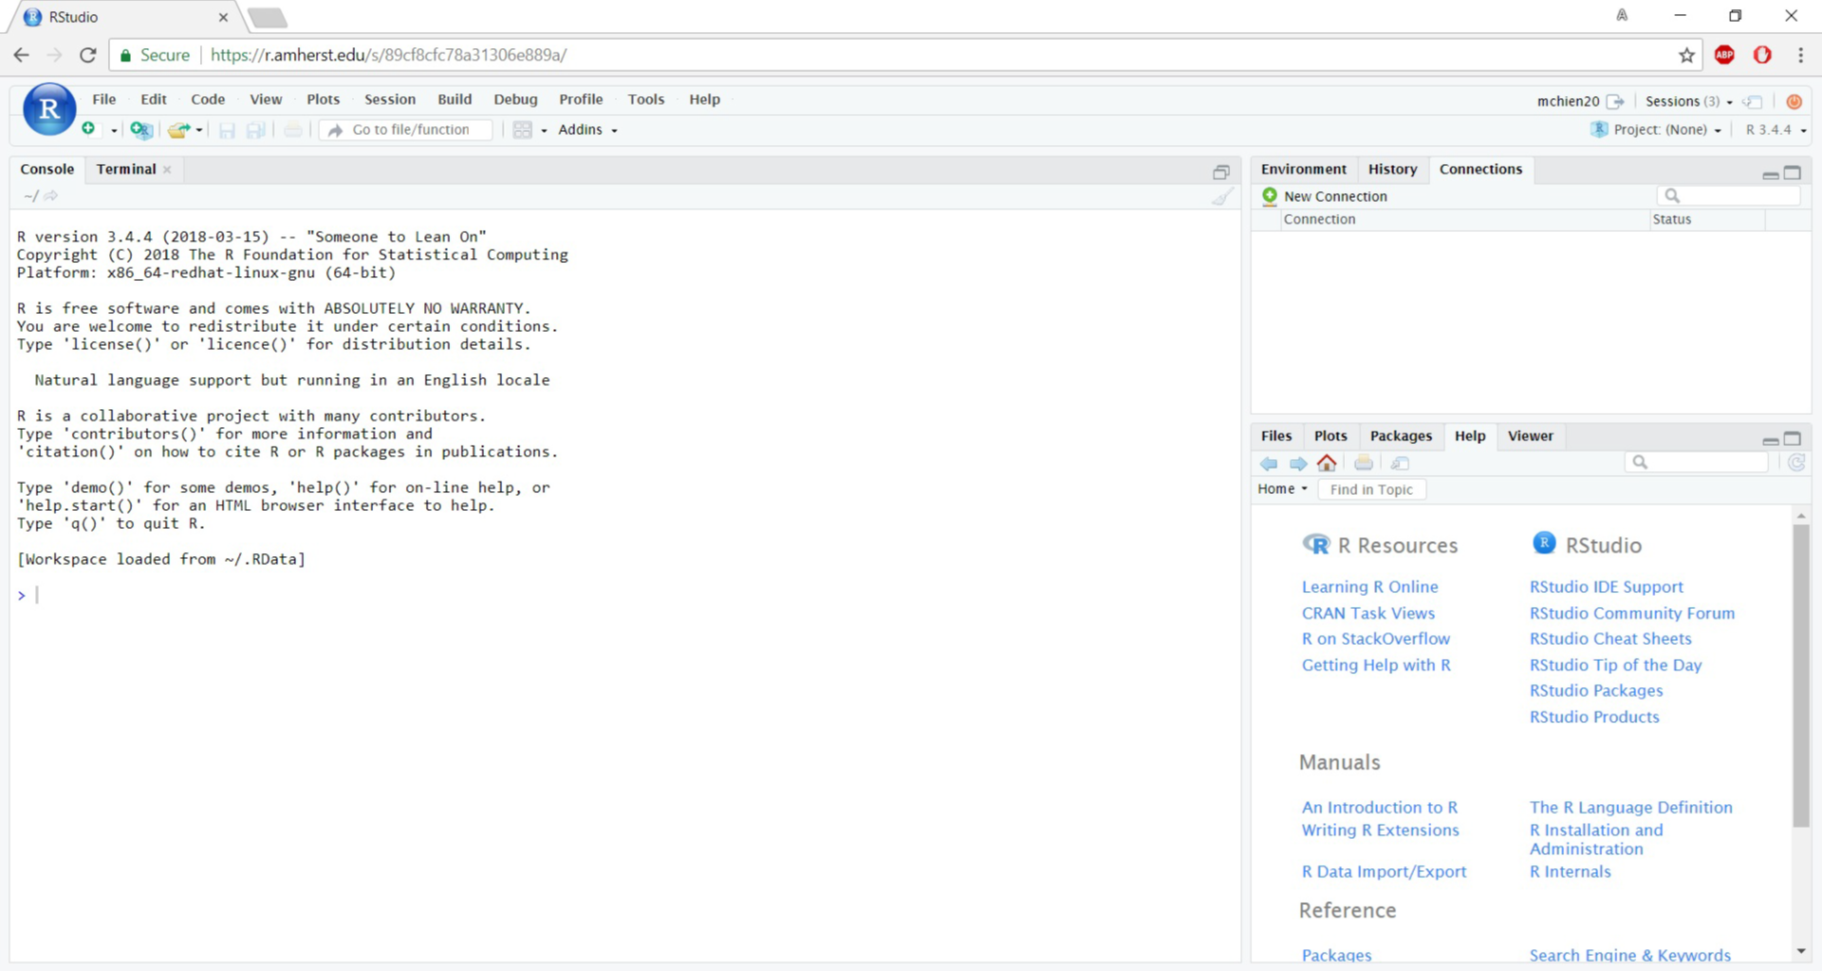
\includegraphics[width=\textwidth]{images/rstudio-cloud-interface} \end{center}

Sie können feststellen, dass \textsf{RStudio} seine Welt in vier \emph{Panel} aufteilt. Verschiedende \emph{Panel} sind weiter unterteilt in mehrere Reiter. Welche Reiter in welchem \emph{Panel} auftauchen kann vom Nutzer konfiguriert werden.

\textsf{R} kann vieles mehr als ein einfacher Taschenrechner und wir werden zu gegebener Zeit zusätzliche Eigenschaften vorstellen. Aber, das Durchführen von einfachen Berechnungen in \textsf{R} ist eine gute Vorgehensweise, um die Eigenschaften von \textsf{RStudio} kennenzulernen.

Befehle, die in dem Reiter \textsc{Console} eingetragen werden, werden direkt ausgeführt von \textsf{R}. Ein guter Start, sich mit der Konsole vertraut zu machen, ist einfache Berechnungen ähnlich wie mit einem Taschenrechner auszuführen. Das meiste funktioniert analog zum typischen Taschenrechner.

Geben Sie folgende Befehle in der Konsole ein:

\begin{Shaded}
\begin{Highlighting}[]
\DecValTok{5} \SpecialCharTok{+} \DecValTok{3}
\end{Highlighting}
\end{Shaded}

\begin{verbatim}
[1] 8
\end{verbatim}

\begin{Shaded}
\begin{Highlighting}[]
\FloatTok{15.3} \SpecialCharTok{*} \FloatTok{23.4}
\end{Highlighting}
\end{Shaded}

\begin{verbatim}
[1] 358.02
\end{verbatim}

\begin{Shaded}
\begin{Highlighting}[]
\FunctionTok{sqrt}\NormalTok{(}\DecValTok{16}\NormalTok{)    }\CommentTok{\# Quadratwurzel}
\end{Highlighting}
\end{Shaded}

\begin{verbatim}
[1] 4
\end{verbatim}

Dieses letzte Beispiel zeigt, wie Funktionen in \textsf{R} aufgerufen werden und wie Kommentare verwendet werden. Das \texttt{\#}-Zeichen muss einem Kommentar vorhergehen. Kommentare können sehr nützlich sein bei Skripten mit mehreren Befehlen oder um Code zu erklären.

Werte können zur späteren Weiterverarbeitung mit Variablennamen abgespeichert werden.

\begin{note}{note}
Es ist wahrscheinlich am sinnvollsten, sich auf eine Vorgehensweise zwischen rechts-nach-links Zuweisung oder umgekehrt festzulegen, statt hin und her zu wechseln. Wir bevorzugen den Pfeiloperator, weil es visuell darstellt, was in einer Zuweisung passiert und weil es eine klare Unterscheidung zum Zuweisungsoperator darstellt, die Verwendung von \texttt{=} weist Variablen Werte zu und die Verwendung von \texttt{==} testet auf Gleichheit von Werten.

\end{note}

\begin{Shaded}
\begin{Highlighting}[]
\NormalTok{product }\OtherTok{=} \FloatTok{15.3} \SpecialCharTok{*} \FloatTok{23.4}       \CommentTok{\# Speichere das Ergebnis}
\NormalTok{product                     }\CommentTok{\# Zeige das Ergebnis an}
\end{Highlighting}
\end{Shaded}

\begin{verbatim}
[1] 358.02
\end{verbatim}

\begin{Shaded}
\begin{Highlighting}[]
\NormalTok{product }\OtherTok{\textless{}{-}} \FloatTok{15.3} \SpecialCharTok{*} \FloatTok{23.4}      \CommentTok{\# \textless{}{-} kann verwendet werden statt =}
\NormalTok{product  }
\end{Highlighting}
\end{Shaded}

\begin{verbatim}
[1] 358.02
\end{verbatim}

Sobald Variablen definiert sind, können sie in anderen Operationen und Funktionen verwendet werden.

\begin{Shaded}
\begin{Highlighting}[]
\FloatTok{0.5} \SpecialCharTok{*}\NormalTok{ product               }\CommentTok{\# Die Hälfte von product}
\end{Highlighting}
\end{Shaded}

\begin{verbatim}
[1] 179.01
\end{verbatim}

\begin{Shaded}
\begin{Highlighting}[]
\FunctionTok{log}\NormalTok{(product)                }\CommentTok{\# (natürlicher) Logarithmus von product}
\end{Highlighting}
\end{Shaded}

\begin{verbatim}
[1] 5.880589
\end{verbatim}

\begin{Shaded}
\begin{Highlighting}[]
\FunctionTok{log10}\NormalTok{(product)              }\CommentTok{\# Logarithmus zur Basis 10 von product}
\end{Highlighting}
\end{Shaded}

\begin{verbatim}
[1] 2.553907
\end{verbatim}

\begin{Shaded}
\begin{Highlighting}[]
\FunctionTok{log2}\NormalTok{(product)               }\CommentTok{\# Logarithmus zur Basis 2 von product}
\end{Highlighting}
\end{Shaded}

\begin{verbatim}
[1] 8.483896
\end{verbatim}

\begin{Shaded}
\begin{Highlighting}[]
\FunctionTok{log}\NormalTok{(product, }\AttributeTok{base =} \DecValTok{2}\NormalTok{)      }\CommentTok{\# Logarithmus zur Basis 2 von product, mit expliziter Angabe der Basis}
\end{Highlighting}
\end{Shaded}

\begin{verbatim}
[1] 8.483896
\end{verbatim}

Das Semikolon kann verwendet werden, um mehrere Befehle in einer Zeile zu schreiben.\\
Eine übliche Anwendung davon ist es, das Zuweisen eines Ergebnisses und Anzeigen desselben auf einmal zu machen:

\begin{Shaded}
\begin{Highlighting}[]
\NormalTok{product }\OtherTok{\textless{}{-}} \FloatTok{15.3} \SpecialCharTok{*} \FloatTok{23.4}\NormalTok{; product    }\CommentTok{\# Speichere Ergebnis und zeige es an}
\end{Highlighting}
\end{Shaded}

\begin{verbatim}
[1] 358.02
\end{verbatim}

\hypertarget{information-zur-version}{%
\subsection{Information zur Version}\label{information-zur-version}}

Manchmal kann es nützlich sein zu prüfen, welche Versionen des Paketes \texttt{mosaic}, von \textsf{R} und
\textsf{RStudio} Sie verwenden. Die Eingabe von \texttt{sessionInfo()} zeigt Informationen über die Version von \textsf{R} und die geladenen Pakete an, während \texttt{RStudio.Version()} die Version von \textsf{RStudio} ausgibt.

\begin{Shaded}
\begin{Highlighting}[]
\FunctionTok{sessionInfo}\NormalTok{()}
\end{Highlighting}
\end{Shaded}

\begin{verbatim}
R version 4.1.0 (2021-05-18)
Platform: x86_64-w64-mingw32/x64 (64-bit)
Running under: Windows 10 x64 (build 18363)

Matrix products: default

locale:
[1] LC_COLLATE=German_Germany.1252  LC_CTYPE=German_Germany.1252   
[3] LC_MONETARY=German_Germany.1252 LC_NUMERIC=C                   
[5] LC_TIME=German_Germany.1252    

attached base packages:
[1] stats     graphics  grDevices utils     datasets  methods   base     

other attached packages:
 [1] kableExtra_1.3.4  mosaic_1.8.3      ggridges_0.5.3    mosaicData_0.20.2
 [5] ggformula_0.10.1  ggstance_0.3.5    dplyr_1.0.7       Matrix_1.3-4     
 [9] ggplot2_3.3.5     lattice_0.20-44   knitr_1.33       

loaded via a namespace (and not attached):
 [1] ggrepel_0.9.1     Rcpp_1.0.6        svglite_2.0.0     tidyr_1.1.3      
 [5] assertthat_0.2.1  digest_0.6.27     utf8_1.2.1        ggforce_0.3.3    
 [9] R6_2.5.0          plyr_1.8.6        backports_1.2.1   labelled_2.8.0   
[13] evaluate_0.14     httr_1.4.2        pillar_1.6.1      rlang_0.4.11     
[17] rstudioapi_0.13   rmarkdown_2.9     splines_4.1.0     webshot_0.5.2    
[21] readr_1.4.0       stringr_1.4.0     htmlwidgets_1.5.3 polyclip_1.10-0  
[25] munsell_0.5.0     broom_0.7.8       compiler_4.1.0    xfun_0.24        
[29] systemfonts_1.0.2 pkgconfig_2.0.3   htmltools_0.5.1.1 tidyselect_1.1.1 
[33] tibble_3.1.2      gridExtra_2.3     mosaicCore_0.9.0  bookdown_0.22    
[37] viridisLite_0.4.0 fansi_0.5.0       crayon_1.4.1      withr_2.4.2      
[41] MASS_7.3-54       grid_4.1.0        gtable_0.3.0      lifecycle_1.0.0  
[45] DBI_1.1.1         magrittr_2.0.1    scales_1.1.1      stringi_1.6.2    
[49] farver_2.1.0      leaflet_2.0.4.1   xml2_1.3.2        ellipsis_0.3.2   
[53] ggdendro_0.1.22   generics_0.1.0    vctrs_0.3.8       tools_4.1.0      
[57] forcats_0.5.1     glue_1.4.2        tweenr_1.0.2      purrr_0.3.4      
[61] hms_1.1.0         crosstalk_1.1.1   yaml_2.2.1        colorspace_2.0-2 
[65] rvest_1.0.0       haven_2.4.1      
\end{verbatim}

\hypertarget{arbeiten-mit-dateien}{%
\section{Arbeiten mit Dateien}\label{arbeiten-mit-dateien}}

\hypertarget{das-arbeiten-mit-r-script-dateien}{%
\subsection{Das Arbeiten mit R-Script Dateien}\label{das-arbeiten-mit-r-script-dateien}}

Eine Alternative ist es, \textsf{R}-Befehle in eine Datei zu speichern. \textsf{RStudio} bietet einen integrierten Editor um diese Dateien zu bearbeiten und unterstützt die Ausführung eines Teils oder aller Befehle.
Um eine Datei zu erstellen, gehen Sie in der Menüleiste auf \textsc{File}, dann \textsc{New File} und dann \textsc{R Script}. Es öffnet sich ein Datei-Editor Fenster im \textsc{Source} Panel.
Hier kann \textsf{R}-Code eingetragen werden und es stehen Schaltflächen und Menüpunkte zur Verfügung, um den gesamten Code (das sogenannte \emph{Sourcing} der Datei), einzelne Zeilen oder einen ausgewählten Abschnitt der Datei auszuführen.

\hypertarget{arbeiten-mit-rmarkdown-und-knitrlatex}{%
\subsection{Arbeiten mit RMarkdown und knitr/LaTeX}\label{arbeiten-mit-rmarkdown-und-knitrlatex}}

Eine dritte Alternative ist es \textsf{RStudio}s Unterstützung für reproduzierbare Forschung zu nutzen. Wenn Sie \textsf{LaTeX} schon kennen, werden Sie die Funktionialitäten des integrierten \textsf{knitr/LaTeX} erforschen wollen. Wenn Sie \textsf{LaTeX} noch nicht kennen, dann bietet das einfachere RMarkdown System eine gute Einführung in die Welt der reproduzierbaren Forschung. Es bietet auch eine gute Möglichkeit für Studierende, ihre Hausarbeiten und Berichte zu erstellen, die Text, \textsf{R}-Code, \textsf{R}-Output sowie Abbildungen enthalten. Um eine neue \textsf{R Markdown}-Datei zu erstellen, wählen Sie \textsc{File}, dann \textsc{New File}, dann \textsf{R Markdown}. Die Datei wird mit einer Kurzvorlage geöffnet, welche die Markup-Sprache skizziert.

\begin{center}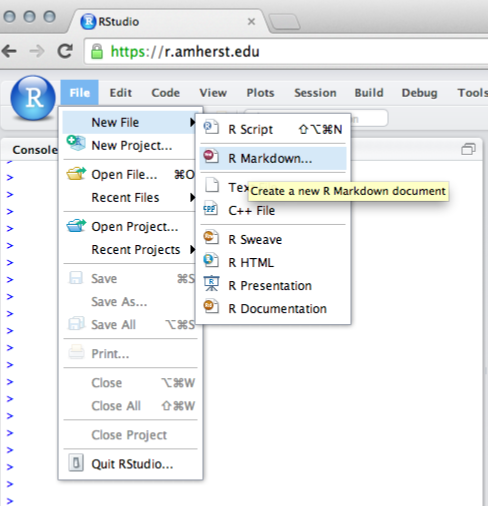
\includegraphics[width=0.4\linewidth]{images/rmarkdown1} \end{center}

Das Paket \texttt{mosaic} enthält zwei nützliche \textsf{R Markdown} Vorlagen für den Einstieg: \texttt{fancy} enthält bereits etwas Schnickschnack (und hat zum Ziel, eine Übersicht der Möglichkeiten zu bieten), während \texttt{plain} nur ein Grundgerüst enthält und nützlich als Startpunkt für eine neue Analyse ist. Auf diese Vorlagen wird mittels der \textsc{Template}-Option bei Erstellung einer neuen \textsf{R Markdown}-Datei zugegriffen:

\begin{center}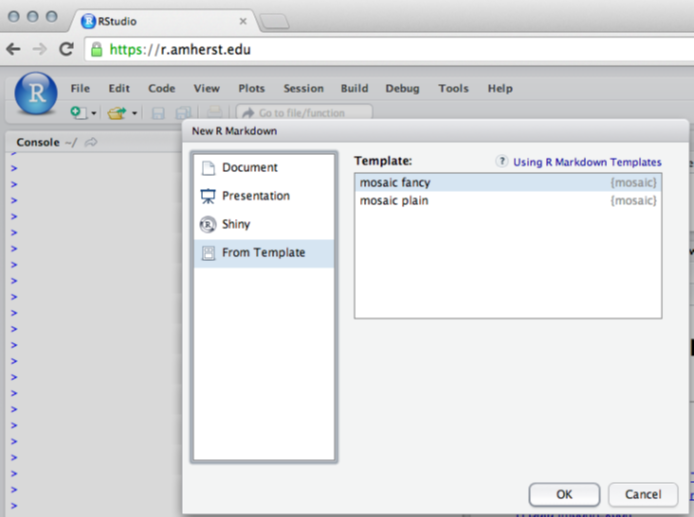
\includegraphics[width=0.5\linewidth]{images/rmarkdown2} \end{center}

Klicken Sie auf die \textsc{Knit}-Schaltfläche, um die Markdown-Datei in eine HTML-, PDF-, oder Word-Datei zu konvertieren:

\begin{center}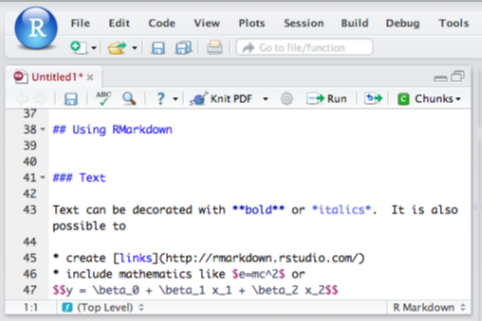
\includegraphics[width=0.5\linewidth]{images/rmarkdown3} \end{center}

Das erzeugt eine formatierte Version des Dokumentes:

\begin{center}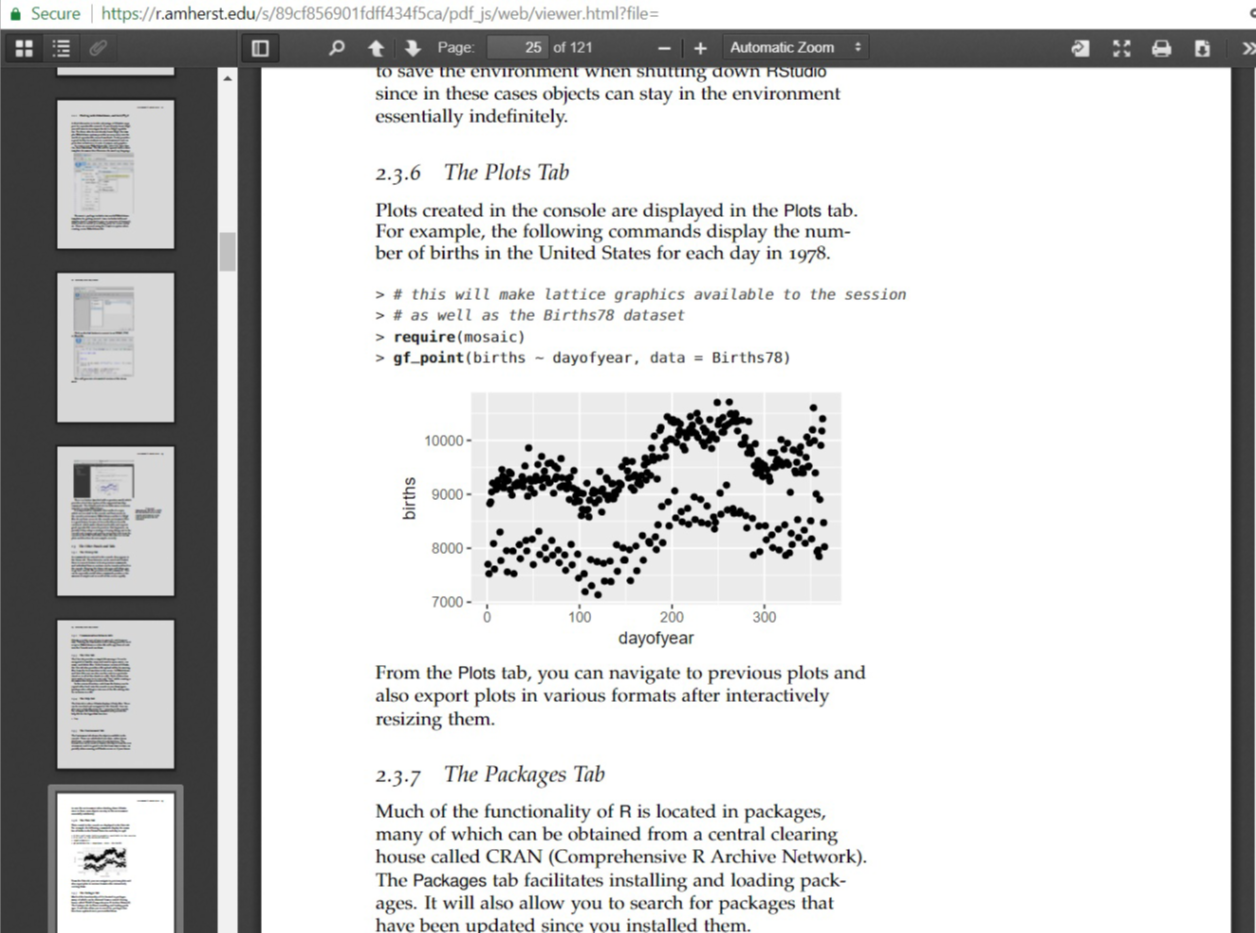
\includegraphics[width=0.9\textwidth]{images/rmarkdown4} \end{center}

Das Hilfemenü enthält eine ``Markdown Quick Reference'' und bietet eine kurze Beschreibung der unterstützten Markup Befehle. Die \textsf{RStudio} Webseite enthält weitere ausführlichere Anleitungen über die Verwendung von \textsf{R Markdown}.

\begin{achtung}{achtung}
\textsf{R Markdown} und \textsf{knitr/LaTeX}-Dateien haben keinen Zugriff auf die \textsc{Console}-Umgebung, weshalb der Code in diesen Dateien eigenständig sein muss.

\end{achtung}

Dass \textsf{R Markdown}- und \textsf{knitr/LaTeX}-Dateien, im Gegensatz zu \textsf{R}-Skripten, die in der \textsc{Console} ausgeführt werden, keinen Zugriff auf die \textsc{Console}-Umgebung haben, ist eine gute Eigenschaft, weil die Dateien deshalb eigenständig sein müssen. Dies ermöglicht die Austauschbarkeit und unterstützt gute reproduzierbare Forschungspraktiken. Anfänger, insbesondere wenn sie Analyseschritte in der Konsole ausprobieren und den Code dann über copy \& paste in die Datei einfügen, werden zunächst noch häufig Dateien kreieren, die nicht vollständig sind und deshalb nicht korrekt kompilieren.

\hypertarget{die-funktionen-der-panel-und-reiter}{%
\section{Die Funktionen der Panel und Reiter}\label{die-funktionen-der-panel-und-reiter}}

\hypertarget{der-history-reiter}{%
\subsection{Der History-Reiter}\label{der-history-reiter}}

Wenn Befehle in der \textsc{Console} eingetragen werden, dann erscheinen Sie in dem \textsc{History}-Reiter. Diese Historie kann gespeichert und geladen werden, es gibt eine Suchfunktion, um vorhergehende Befehle zu finden und einzelne Zeilen oder Abschnitte können zurück an die Konsole geschickt werden. Mit geöffnetem \textsc{History}-Reiter können Sie zurück blättern und auf die vorangegangenen Befehle zugreifen. Das ist vor allem dann nützlich, wenn Befehle viel Output erzeugen und schnell aus dem Bildschirm verschwinden.

\hypertarget{kommunikation-zwischen-reitern}{%
\subsection{Kommunikation zwischen Reitern}\label{kommunikation-zwischen-reitern}}

\textsf{RStudio} bietet verschiedene Möglichkeiten, um \textsf{R}-Code zwischen Reitern auszutauschen. Das Klicken der \textsc{Run}-Schaltfläche im Editor-Fenster für ein \textsf{R}-Skript oder \textsf{R Markdown}- oder andere Datei kopiert Zeilen mit Code in die Konsole und führt sie aus.

\hypertarget{der-file-reiter}{%
\subsection{Der File-Reiter}\label{der-file-reiter}}

Der \textsc{Files}-Reiter bietet eine einfache Dateiverwaltung an. Sie kann auf übliche Weise bedient und genutzt werden, um Dateien zu öffnen, zu verschieben, umzubenennen oder zu löschen. In der Browser-Version von \textsf{RStudio} bietet der \textsc{Files}-Reiter auch die Möglichkeit, Dateien hochzuladen, um Dateien vom lokalen Rechner auf den Server zu verschieben. In \textsf{R Markdown}- und \textsf{knitr}-Dateien kann der Code auch in einem bestimmten Abschnitt (\textsc{chunk}) oder in allen ausgeführt werden. Jede dieser Eigenschaften ermöglicht es Codes ``live'' auszuprobieren und gleichzeitig ein Dokument zu erstellen, das eine Aufzeichnung des verwendeten Codes enthält.
Umgekehrt kann Code aus der \textsc{History} zurück in die Konsole kopiert werden, um die Befehle nochmals auszuführen (ggf. nach Bearbeitung) oder in eine Datei im \textsc{File}-Reiter eingefügt werden.

\hypertarget{der-help-reiter}{%
\subsection{Der Help-Reiter}\label{der-help-reiter}}

In dem \textsc{Help}-Reiter zeigt \textsf{RStudio} die \textsf{R}-Hilfe-Seiten an. Diese können durchsucht und navigiert werden. Sie können auch eine Hilfeseite öffnen, indem Sie den \texttt{?}-Operator in der Konsole verwenden.
Zum Beispiel führt folgender Befehl dazu, dass die Hilfeseite zur Logarithmusfunktion aufgerufen wird:

\begin{Shaded}
\begin{Highlighting}[]
\NormalTok{?log}
\end{Highlighting}
\end{Shaded}

\hypertarget{der-environment-reiter}{%
\subsection{Der Environment-Reiter}\label{der-environment-reiter}}

Der \textsc{Environment}-Reiter zeigt die Objekte, die für die \textsc{Console} zur Verfügung stehen. Diese sind unterteilt in Daten, Werte (Objekte die weder Dataframe noch Funktionen sind) und Funktionen. Die ``Besen''-Schaltfläche kann verwendet werden, um alle Objekte aus der Umgebung zu entfernen und es ist empfehlenswert, das ab und zu durchzuführen, vor allem dann, wenn Sie auf dem \textsf{RStudio} Server arbeiten oder wenn Sie sich dafür entscheiden, die Umgebung beim Schließen von \textsf{RStudio} abzuspeichern. In diesen Fällen könnten die Objekte sonst quasi ewig in der Umgebung gespeichert bleiben.

\hypertarget{der-plots-reiter}{%
\subsection{Der Plots-Reiter}\label{der-plots-reiter}}

Diagramme, die in der Konsole erzeugt werden, werden im \textsc{Plots}-Reiter angezeigt. Zum Beispiel zeigen die folgenden Befehle die Anzahl der Geburten in den Vereinigten Staaten für jeden Tag aus 1978 an:

\begin{Shaded}
\begin{Highlighting}[]
\FunctionTok{library}\NormalTok{(mosaic)}
\FunctionTok{gf\_point}\NormalTok{(births }\SpecialCharTok{\textasciitilde{}}\NormalTok{ day\_of\_year, }\AttributeTok{data =}\NormalTok{ Births78) }
\end{Highlighting}
\end{Shaded}

\begin{center}\includegraphics[width=0.6\linewidth]{Mosaic-Handbuch_files/figure-latex/unnamed-chunk-15-1} \end{center}

Innerhalb des \textsc{Plots}-Reiters haben Sie Zugriff auf vorherige Grafiken und Sie können diese, nach interaktiver Größenanpassung, in verschiedenen Formaten exportieren.

\hypertarget{der-packages-reiter}{%
\subsection{Der Packages-Reiter}\label{der-packages-reiter}}

Ein großer Teil der \textsf{R}-Funktionalitäten befindet sich in Paketen, die meistens über eine zentrale Anlaufstelle namens CRAN (Comprehensive \textsf{R} Archive Network) verfügbar sind. Der \textsc{Packages}-Reiter vereinfacht die Installation und das Laden der Pakete. Er ermöglicht es auch Pakete zu finden, die seit ihrer Installation ein Update bekommen haben.

\hypertarget{metrVar}{%
\chapter{Eine metrische Variable}\label{metrVar}}

\hypertarget{numerische-zusammenfassungen}{%
\section{Numerische Zusammenfassungen}\label{numerische-zusammenfassungen}}

\textsf{R} beinhaltet eine Reihe von Befehlen, um numerische Variablen zusammenzufassen. Diese beinhalten das Berechnen von Mittelwert, Standardabweichung, Varianz, Median, Interquartilsabstand (IQR) sowie frei wählbare Quantile. Wir werden diese am CESD-Maß (\emph{Center for Epidemiologic Studies-Depression}) für depressive Symptome demonstrieren (diese Werte liegen zwischen \(0\) und \(60\); höhere Werte stehen für mehr depressive Symptome).
Um die Lesbarkeit der Ausgabe zu verbessern, werden wir die Zahl der ausgegebenen Ziffern begrenzen (s. \texttt{?options()} für weitere Konfigurationsmöglichkeiten).

\begin{Shaded}
\begin{Highlighting}[]
\FunctionTok{library}\NormalTok{(mosaic)}
\FunctionTok{options}\NormalTok{(}\AttributeTok{digits =} \DecValTok{4}\NormalTok{)}
\FunctionTok{mean}\NormalTok{(}\SpecialCharTok{\textasciitilde{}}\NormalTok{cesd, }\AttributeTok{data =}\NormalTok{ HELPrct)}
\end{Highlighting}
\end{Shaded}

\begin{verbatim}
[1] 32.85
\end{verbatim}

Beachten Sie, dass die Funktion \texttt{mean()} im Paket \texttt{mosaic} eine Formel-Schnittstelle beinhaltet, die \texttt{lattice}-Grafiken und linearen Modellen (z. B. \texttt{lm()} ) ähnlich ist. Das Paket \texttt{mosaic} stellt viele weitere Funktionen zur Verfügung, die die gleiche Notation verwenden wie wir in diesem Buch.

\begin{tiefereinsteigen}{tiefereinsteigen}
Wenn Sie mit der Notation der Formeln noch nicht vertraut sind, bietet das Begleitbuch \emph{Start Teaching with R} \autocite{TeachingR} eine detaillierte Präsentation. \emph{Start Modeling with R} \autocite{ModelingR}, ein anderes Begleitbuch, vertieft die Beziehung zwischen dem Modellierungsprozess und der Notation der Formeln.

\end{tiefereinsteigen}

Dieselbe Ausgabe könnte auch durch die folgenden Befehle erzeugt werden (aber wir werden die MOSAIC-Versionen verwenden, wann immer möglich):

\begin{Shaded}
\begin{Highlighting}[]
\FunctionTok{with}\NormalTok{(HELPrct, }\FunctionTok{mean}\NormalTok{(cesd))}
\end{Highlighting}
\end{Shaded}

\begin{verbatim}
[1] 32.85
\end{verbatim}

\begin{Shaded}
\begin{Highlighting}[]
\FunctionTok{mean}\NormalTok{(HELPrct}\SpecialCharTok{$}\NormalTok{cesd)}
\end{Highlighting}
\end{Shaded}

\begin{verbatim}
[1] 32.85
\end{verbatim}

Eine ähnliche Funktionalität gibt es auch für andere zusammenfassende Statistiken:

\begin{Shaded}
\begin{Highlighting}[]
\FunctionTok{sd}\NormalTok{(}\SpecialCharTok{\textasciitilde{}}\NormalTok{ cesd, }\AttributeTok{data=}\NormalTok{HELPrct)}
\end{Highlighting}
\end{Shaded}

\begin{verbatim}
[1] 12.51
\end{verbatim}

\begin{Shaded}
\begin{Highlighting}[]
\FunctionTok{sd}\NormalTok{(}\SpecialCharTok{\textasciitilde{}}\NormalTok{ cesd, }\AttributeTok{data=}\NormalTok{HELPrct)}\SpecialCharTok{\^{}}\DecValTok{2}
\end{Highlighting}
\end{Shaded}

\begin{verbatim}
[1] 156.6
\end{verbatim}

\begin{Shaded}
\begin{Highlighting}[]
\FunctionTok{var}\NormalTok{(}\SpecialCharTok{\textasciitilde{}}\NormalTok{ cesd, }\AttributeTok{data=}\NormalTok{HELPrct)}
\end{Highlighting}
\end{Shaded}

\begin{verbatim}
[1] 156.6
\end{verbatim}

\begin{Shaded}
\begin{Highlighting}[]
\FunctionTok{median}\NormalTok{(}\SpecialCharTok{\textasciitilde{}}\NormalTok{ cesd, }\AttributeTok{data=}\NormalTok{HELPrct)}
\end{Highlighting}
\end{Shaded}

\begin{verbatim}
[1] 34
\end{verbatim}

Nach dem gleichen Muster lassen sich auch Quantile der Verteilung berechnen:

Standardmäßig stellt die Funktion \texttt{quantile()} die Quartile dar, aber ihr kann auch ein Vektor der gewünschten Quantile übergeben werden:

\begin{Shaded}
\begin{Highlighting}[]
\FunctionTok{with}\NormalTok{(HELPrct, }\FunctionTok{quantile}\NormalTok{(cesd))}
\end{Highlighting}
\end{Shaded}

\begin{verbatim}
  0%  25%  50%  75% 100% 
   1   25   34   41   60 
\end{verbatim}

\begin{Shaded}
\begin{Highlighting}[]
\FunctionTok{with}\NormalTok{(HELPrct, }\FunctionTok{quantile}\NormalTok{(cesd, }\FunctionTok{c}\NormalTok{(.}\DecValTok{025}\NormalTok{, .}\DecValTok{975}\NormalTok{)))}
\end{Highlighting}
\end{Shaded}

\begin{verbatim}
 2.5% 97.5% 
  6.3  55.0 
\end{verbatim}

\begin{achtung}{achtung}
Nicht alle Befehle wurden schon für die Nutzung des Formel-Interfaces überarbeitet. Für diese Funktionen muss für den Zugriff auf Variablen innerhalb eines Datensatzes \texttt{with()} oder das \$-Zeichen genutzt werden.

\end{achtung}

Schließlich stellt die Funktion \texttt{favstats()} (für favorite stats) im Paket \texttt{mosaic} eine prägnante Zusammenfassung einiger nützlicher Kennzahlen.

\begin{Shaded}
\begin{Highlighting}[]
\FunctionTok{favstats}\NormalTok{(}\SpecialCharTok{\textasciitilde{}}\NormalTok{cesd, }\AttributeTok{data =}\NormalTok{ HELPrct)}
\end{Highlighting}
\end{Shaded}

\begin{verbatim}
 min Q1 median Q3 max  mean    sd   n missing
   1 25     34 41  60 32.85 12.51 453       0
\end{verbatim}

\hypertarget{grafische-zusammenfassungen}{%
\section{Grafische Zusammenfassungen}\label{grafische-zusammenfassungen}}

Die Funktion \texttt{histogram()} wird genutzt, um ein Histogramm zu erzeugen. Hier nutzen wir das Formel-Interface (wie im Buch \emph{Start Modeling with R} \autocite{TeachingR}) um ein Histogramm der CESD-Werte zu erzeugen.

\begin{Shaded}
\begin{Highlighting}[]
\FunctionTok{gf\_histogram}\NormalTok{(}\SpecialCharTok{\textasciitilde{}}\NormalTok{ cesd, }\AttributeTok{data =}\NormalTok{ HELPrct, }\AttributeTok{binwidth =} \FloatTok{5.9}\NormalTok{)}
\end{Highlighting}
\end{Shaded}

\begin{center}\includegraphics[width=0.6\linewidth]{Mosaic-Handbuch_files/figure-latex/unnamed-chunk-22-1} \end{center}

Wir können die Optionen \texttt{binwidth()} und \texttt{center()} nutzen, um die Lage der Säulen zu steuern.

\begin{Shaded}
\begin{Highlighting}[]
\FunctionTok{gf\_histogram}\NormalTok{(}\SpecialCharTok{\textasciitilde{}}\NormalTok{ cesd, }\AttributeTok{data =}\NormalTok{ HELPrct, }\AttributeTok{binwidth =} \DecValTok{5}\NormalTok{, }\AttributeTok{center =} \FloatTok{2.5}\NormalTok{)}
\end{Highlighting}
\end{Shaded}

\begin{center}\includegraphics[width=0.6\linewidth]{Mosaic-Handbuch_files/figure-latex/unnamed-chunk-23-1} \end{center}

Im Datensatz \texttt{HELPrct} ist etwa ein Viertel der Probanden weiblich.

\begin{Shaded}
\begin{Highlighting}[]
\FunctionTok{tally}\NormalTok{( }\SpecialCharTok{\textasciitilde{}}\NormalTok{ sex, }\AttributeTok{data =}\NormalTok{ HELPrct)}
\end{Highlighting}
\end{Shaded}

\begin{verbatim}
sex
female   male 
   107    346 
\end{verbatim}

\begin{Shaded}
\begin{Highlighting}[]
\FunctionTok{tally}\NormalTok{( }\SpecialCharTok{\textasciitilde{}}\NormalTok{ sex, }\AttributeTok{format =} \StringTok{"percent"}\NormalTok{, }\AttributeTok{data =}\NormalTok{ HELPrct)}
\end{Highlighting}
\end{Shaded}

\begin{verbatim}
sex
female   male 
 23.62  76.38 
\end{verbatim}

Es ist unkompliziert die Analyse nur auf die weiblichen Probanden zu beschränken. Wenn wir viele Analysen mit einer Teilgruppe unserer Daten durchführen wollen, könnte es am leichtesten sein, einen neuen Datensatz zu erzeugen, der nur die Fälle enthält, die uns interessieren. Die Funktion \texttt{filter()} im Paket \texttt{dplyr} kann genutzt werden, um einen solchen Datensatz zu erzeugen, der nur die Frauen oder nur die Männer enthält (s. auch Kapitel \ref{subdaten}). Nachdem dieser erzeugt ist, wird die Funktion \texttt{stem()} genutzt, um ein Stamm-Blatt-Diagramm (\emph{stem and leaf plot}) zu erzeugen.

\begin{Shaded}
\begin{Highlighting}[]
\NormalTok{Female }\OtherTok{\textless{}{-}} \FunctionTok{filter}\NormalTok{(HELPrct, sex }\SpecialCharTok{==} \StringTok{\textquotesingle{}female\textquotesingle{}}\NormalTok{)}
\NormalTok{Male }\OtherTok{\textless{}{-}} \FunctionTok{filter}\NormalTok{(HELPrct, sex }\SpecialCharTok{==} \StringTok{\textquotesingle{}male\textquotesingle{}}\NormalTok{)}
\FunctionTok{with}\NormalTok{(Female, }\FunctionTok{stem}\NormalTok{(cesd))}
\end{Highlighting}
\end{Shaded}

\begin{verbatim}
The decimal point is 1 digit(s) to the right of the |

0 | 3
0 | 567
1 | 3
1 | 555589999
2 | 123344
2 | 66889999
3 | 0000233334444
3 | 5556666777888899999
4 | 00011112222334
4 | 555666777889
5 | 011122222333444
5 | 67788
6 | 0
\end{verbatim}

\begin{achtung}{achtung}
Um Gleichheit von Ausprägungen zu überprüfen wird ein doppeltes Gleichheitszeichen genutzt!

\end{achtung}

Teilgruppen können auch innerhalb eines Befehls erzeugt werden (dieses Mal mit einer überlagerten Normalverteilung):

\begin{Shaded}
\begin{Highlighting}[]
\FunctionTok{gf\_dhistogram}\NormalTok{(}\SpecialCharTok{\textasciitilde{}}\NormalTok{ cesd, }\AttributeTok{data =} \FunctionTok{filter}\NormalTok{(HELPrct, sex }\SpecialCharTok{==} \StringTok{"female"}\NormalTok{),}
\AttributeTok{binwidth =} \FloatTok{7.1}\NormalTok{) }\SpecialCharTok{\%\textgreater{}\%}
\FunctionTok{gf\_fitdistr}\NormalTok{(}\AttributeTok{dist =} \StringTok{"dnorm"}\NormalTok{)}
\end{Highlighting}
\end{Shaded}

\begin{center}\includegraphics[width=0.6\linewidth]{Mosaic-Handbuch_files/figure-latex/unnamed-chunk-27-1} \end{center}

Alternativ können wir nebeneinander angeordnete Plots erzeugen, um mehre Teilgruppen zu vergleichen.

\begin{Shaded}
\begin{Highlighting}[]
\FunctionTok{gf\_dhistogram}\NormalTok{(}\SpecialCharTok{\textasciitilde{}}\NormalTok{ cesd, }\AttributeTok{data =}\NormalTok{ HELPrct, }\AttributeTok{binwidth =} \FloatTok{5.9}\NormalTok{) }\SpecialCharTok{\%\textgreater{}\%}
\FunctionTok{gf\_facet\_wrap}\NormalTok{(}\SpecialCharTok{\textasciitilde{}}\NormalTok{ sex)}
\end{Highlighting}
\end{Shaded}

\begin{center}\includegraphics[width=0.6\linewidth]{Mosaic-Handbuch_files/figure-latex/unnamed-chunk-28-1} \end{center}

Das Layout kann auch anders angeordnet werden.

\begin{Shaded}
\begin{Highlighting}[]
\FunctionTok{gf\_dhistogram}\NormalTok{(}\SpecialCharTok{\textasciitilde{}}\NormalTok{ cesd, }\AttributeTok{data =}\NormalTok{ HELPrct, }\AttributeTok{binwidth =} \FloatTok{5.9}\NormalTok{) }\SpecialCharTok{\%\textgreater{}\%}
\FunctionTok{gf\_facet\_wrap}\NormalTok{(}\SpecialCharTok{\textasciitilde{}}\NormalTok{ sex, }\AttributeTok{nrow =} \DecValTok{2}\NormalTok{)}
\end{Highlighting}
\end{Shaded}

\begin{center}\includegraphics[width=0.6\linewidth]{Mosaic-Handbuch_files/figure-latex/unnamed-chunk-29-1} \end{center}

Wir können die Zahl der Säulen auf verschiedene Arten steuern. Hierzu wird die Gesamtzahl angegeben.

\begin{Shaded}
\begin{Highlighting}[]
\FunctionTok{gf\_dhistogram}\NormalTok{(}\SpecialCharTok{\textasciitilde{}}\NormalTok{ cesd, }\AttributeTok{bins =} \DecValTok{20}\NormalTok{, }\AttributeTok{data =}\NormalTok{ Female)}
\end{Highlighting}
\end{Shaded}

\begin{center}\includegraphics[width=0.6\linewidth]{Mosaic-Handbuch_files/figure-latex/unnamed-chunk-30-1} \end{center}

Auch die Breite der Säulen kann vorgegeben werden.

\begin{Shaded}
\begin{Highlighting}[]
\FunctionTok{gf\_dhistogram}\NormalTok{(}\SpecialCharTok{\textasciitilde{}}\NormalTok{ cesd, }\AttributeTok{binwidth =} \DecValTok{2}\NormalTok{, }\AttributeTok{data =}\NormalTok{ Female)}
\end{Highlighting}
\end{Shaded}

\begin{center}\includegraphics[width=0.6\linewidth]{Mosaic-Handbuch_files/figure-latex/unnamed-chunk-31-1} \end{center}

Die Funktion \texttt{dotplot()} wird genutzt, um einen \emph{dotplot} für eine kleinere Teilgruppe zu erzeugen (obdachlose Frauen). Wir zeigen auch, wie die Beschriftung der x-Achse geändert werden kann.

\begin{Shaded}
\begin{Highlighting}[]
\FunctionTok{gf\_dotplot}\NormalTok{(}\SpecialCharTok{\textasciitilde{}}\NormalTok{ cesd, }\AttributeTok{binwidth =} \DecValTok{3}\NormalTok{,}
\AttributeTok{data =} \FunctionTok{filter}\NormalTok{(HELPrct, sex }\SpecialCharTok{==} \StringTok{"female"}\NormalTok{, homeless }\SpecialCharTok{==} \StringTok{"homeless"}\NormalTok{)) }\SpecialCharTok{\%\textgreater{}\%}
\FunctionTok{gf\_labs}\NormalTok{(}\AttributeTok{x =} \StringTok{"CESD score"}\NormalTok{)}
\end{Highlighting}
\end{Shaded}

\begin{center}\includegraphics[width=0.6\linewidth]{Mosaic-Handbuch_files/figure-latex/unnamed-chunk-32-1} \end{center}

\hypertarget{dichtekurven}{%
\section{Dichtekurven}\label{dichtekurven}}

Ein Nachteil von Histogrammen besteht darin, dass sie abhängig von der gewählten Anzahl von Säulen sind. Eine andere Darstellung ist die Dichtekurve.

\begin{note}{note}
Dichteplots sind ebenfalls abhängig von diversen Optionen. Wenn Ihr Dichteplot zu zerklüftet oder zu glatt ist, versuchen Sie, das \texttt{adjust}-Argument zu variieren: größer als 1 für glattere Plots, kleiner als 1 für gezacktere Plots.

\end{note}

\begin{tiefereinsteigen}{tiefereinsteigen}
Die Funktion \texttt{plotFun()} kann für Anmerkungen an Plots genutzt werden (s. Kapitel \ref{VisReg}).

\end{tiefereinsteigen}

Hier verzieren wir einen Dichteplot mit einigen Zusätzen, um zu zeigen, wie eine Grafik für didaktische Ziele aufgebaut wird. Wir fügen Text hinzu, legen eine Normalverteilung darüber und ergänzen eine vertikale Linie. Eine Vielzahl von Linienarten, -farben und -stärken stehen zur Auswahl.

\hypertarget{huxe4ufigkeitspolygone}{%
\section{Häufigkeitspolygone}\label{huxe4ufigkeitspolygone}}

Eine dritte Option ist ein Häufigkeitspolygon, bei dem die Grafik erzeugt wird, indem die Mittelpunkte der Säulen eines Histogramms miteinander verbunden werden.

\begin{Shaded}
\begin{Highlighting}[]
\FunctionTok{gf\_freqpoly}\NormalTok{(}\SpecialCharTok{\textasciitilde{}}\NormalTok{ cesd, }\AttributeTok{data =}\NormalTok{ Female, }\AttributeTok{binwidth =} \FloatTok{3.8}\NormalTok{)}
\end{Highlighting}
\end{Shaded}

\begin{center}\includegraphics[width=0.6\linewidth]{Mosaic-Handbuch_files/figure-latex/unnamed-chunk-34-1} \end{center}

\hypertarget{normalverteilungen}{%
\section{Normalverteilungen}\label{normalverteilungen}}

Die berühmteste Dichtekurve ist die Normalverteilung.

Die Funktion \texttt{xpnorm()} erzeugt die Wahrscheinlichkeit, dass eine Zufallsvariable kleiner als das erste Argument ist, bei einer Normalverteilung mit dem Mittelwert als zweitem und der Standardabweichung als drittem Argument. Mehr Informationen über Normalverteilungen sind in Kapitel \ref{powerberechnung} zu finden.

\begin{Shaded}
\begin{Highlighting}[]
\FunctionTok{xpnorm}\NormalTok{(}\FloatTok{1.96}\NormalTok{, }\AttributeTok{mean =} \DecValTok{0}\NormalTok{, }\AttributeTok{sd =} \DecValTok{1}\NormalTok{)}
\end{Highlighting}
\end{Shaded}

\begin{center}\includegraphics[width=0.6\linewidth]{Mosaic-Handbuch_files/figure-latex/unnamed-chunk-35-1} \end{center}

\begin{verbatim}
[1] 0.975
\end{verbatim}

\begin{hinweis}{hinweis}
x steht für eXtra (außerhalb).

\end{hinweis}

\hypertarget{bootstrap}{%
\section{Inferenz einer einzelnen Stichprobe}\label{bootstrap}}

Das 95\%-Konfidenzintervall für den Mittelwert des CESD-Wertes der Frauen kann mit einem t-Test berechnet werden:

\begin{Shaded}
\begin{Highlighting}[]
\FunctionTok{t.test}\NormalTok{( }\SpecialCharTok{\textasciitilde{}}\NormalTok{ cesd, }\AttributeTok{data =}\NormalTok{ Female)}
\end{Highlighting}
\end{Shaded}

\begin{verbatim}
    One Sample t-test

data:  cesd
t = 29, df = 106, p-value <2e-16
alternative hypothesis: true mean is not equal to 0
95 percent confidence interval:
 34.39 39.38
sample estimates:
mean of x 
    36.89 
\end{verbatim}

\begin{Shaded}
\begin{Highlighting}[]
\FunctionTok{confint}\NormalTok{(}\FunctionTok{t.test}\NormalTok{( }\SpecialCharTok{\textasciitilde{}}\NormalTok{ cesd, }\AttributeTok{data =}\NormalTok{ Female))}
\end{Highlighting}
\end{Shaded}

\begin{verbatim}
  mean of x lower upper level
1     36.89 34.39 39.38  0.95
\end{verbatim}

Aber es ist genauso zielführend, es mit der Bootstrap-Methode zu berechnen. Die Statistik, die wir resampeln wollen, ist der Mittelwert.

\begin{tiefereinsteigen}{tiefereinsteigen}
Mehr Details und Beispiele finden sich in der Vignette zum Resampling im Paket \texttt{mosaic}.

\end{tiefereinsteigen}

\begin{Shaded}
\begin{Highlighting}[]
\FunctionTok{mean}\NormalTok{( }\SpecialCharTok{\textasciitilde{}}\NormalTok{ cesd, }\AttributeTok{data =}\NormalTok{ Female)}
\end{Highlighting}
\end{Shaded}

\begin{verbatim}
[1] 36.89
\end{verbatim}

Ein erstes Resampeln führt zu diesem Ergebnis

\begin{Shaded}
\begin{Highlighting}[]
\FunctionTok{mean}\NormalTok{( }\SpecialCharTok{\textasciitilde{}}\NormalTok{ cesd, }\AttributeTok{data =} \FunctionTok{resample}\NormalTok{(Female))}
\end{Highlighting}
\end{Shaded}

\begin{verbatim}
[1] 36.46
\end{verbatim}

\begin{hinweis}{hinweis}
Hier resampeln wir durch Ersetzen des Original-Datensatzes, indem wir einen Pseudo-Zufalls-Datensatz mit der gleichen Anzahl von Zeilen erzeugen.

\end{hinweis}

\begin{note}{hinweis}
Auch wenn eine einzige Stichprobe von geringem Nutzen ist, so ist es doch sinnvoll, die Studierenden die Berechnung durchführen zu lassen, um zu zeigen, dass sie (normalerweise!) ein anderes Ergebnis erhalten als ohne Resampling.

\end{note}

Eine weitere Durchführung wird zu einem anderen Ergebnis führen:

\begin{Shaded}
\begin{Highlighting}[]
\FunctionTok{mean}\NormalTok{( }\SpecialCharTok{\textasciitilde{}}\NormalTok{ cesd, }\AttributeTok{data =} \FunctionTok{resample}\NormalTok{(Female))}
\end{Highlighting}
\end{Shaded}

\begin{verbatim}
[1] 35.23
\end{verbatim}

Jetzt resampeln wir 1000 Stichproben und speichern das Ergebnis in einem Objekt namens \texttt{trials}:

\begin{Shaded}
\begin{Highlighting}[]
\NormalTok{trials }\OtherTok{\textless{}{-}} \FunctionTok{do}\NormalTok{(}\DecValTok{1000}\NormalTok{) }\SpecialCharTok{*} \FunctionTok{mean}\NormalTok{( }\SpecialCharTok{\textasciitilde{}}\NormalTok{ cesd, }\AttributeTok{data =} \FunctionTok{resample}\NormalTok{(Female))}
\FunctionTok{head}\NormalTok{(trials, }\DecValTok{3}\NormalTok{)}
\end{Highlighting}
\end{Shaded}

\begin{verbatim}
   mean
1 38.14
2 37.93
3 35.73
\end{verbatim}

\begin{Shaded}
\begin{Highlighting}[]
\FunctionTok{qdata}\NormalTok{( }\SpecialCharTok{\textasciitilde{}}\NormalTok{ mean, }\FunctionTok{c}\NormalTok{(.}\DecValTok{025}\NormalTok{, .}\DecValTok{975}\NormalTok{), }\AttributeTok{data =}\NormalTok{ trials)}
\end{Highlighting}
\end{Shaded}

\begin{verbatim}
 2.5% 97.5% 
34.29 39.22 
\end{verbatim}

\hypertarget{eine-kategoriale-variable}{%
\chapter{Eine kategoriale Variable}\label{eine-kategoriale-variable}}

\hypertarget{analyse-kategorialer-daten}{%
\section{Analyse kategorialer Daten}\label{analyse-kategorialer-daten}}

Mit Hilfe der Funktion \texttt{tally()} können absolute und relative Häufigkeiten für kategoriale Daten angegeben werden.

\begin{tiefereinsteigen}{tiefereinsteigen}
Im Begleitbuch \emph{Start Teaching with R} \autocite{TeachingR} wird die Formelschreibweise erklärt, die hier ebenfalls verwendet wird. Siehe ebenfalls dort zum Thema statistische Modellierung.

\end{tiefereinsteigen}

\begin{Shaded}
\begin{Highlighting}[]
\FunctionTok{tally}\NormalTok{( }\SpecialCharTok{\textasciitilde{}}\NormalTok{ homeless, }\AttributeTok{data =}\NormalTok{ HELPrct)}
\end{Highlighting}
\end{Shaded}

\begin{verbatim}
homeless
homeless   housed 
     209      244 
\end{verbatim}

\begin{Shaded}
\begin{Highlighting}[]
\FunctionTok{tally}\NormalTok{( }\SpecialCharTok{\textasciitilde{}}\NormalTok{ homeless, }\AttributeTok{margins =} \ConstantTok{TRUE}\NormalTok{, }
       \AttributeTok{data =}\NormalTok{ HELPrct)}
\end{Highlighting}
\end{Shaded}

\begin{verbatim}
homeless
homeless   housed    Total 
     209      244      453 
\end{verbatim}

\begin{Shaded}
\begin{Highlighting}[]
\FunctionTok{tally}\NormalTok{( }\SpecialCharTok{\textasciitilde{}}\NormalTok{ homeless, }\AttributeTok{format =} \StringTok{"percent"}\NormalTok{, }
       \AttributeTok{data =}\NormalTok{ HELPrct)}
\end{Highlighting}
\end{Shaded}

\begin{verbatim}
homeless
homeless   housed 
   46.14    53.86 
\end{verbatim}

\begin{Shaded}
\begin{Highlighting}[]
\FunctionTok{tally}\NormalTok{( }\SpecialCharTok{\textasciitilde{}}\NormalTok{ homeless, }\AttributeTok{format =} \StringTok{"proportion"}\NormalTok{, }
       \AttributeTok{data =}\NormalTok{ HELPrct)}
\end{Highlighting}
\end{Shaded}

\begin{verbatim}
homeless
homeless   housed 
  0.4614   0.5386 
\end{verbatim}

\hypertarget{der-binomialtest}{%
\section{Der Binomialtest}\label{der-binomialtest}}

Ein exaktes Konfidenzintervall für einen Anteilswert (sowie ein Test der Nullhypothese, dass der Bevölkerungsanteil gleich einem bestimmten Wert -- standardmäßig 0.5 -- ist) kann durch die Funktion \texttt{binom.test()} berechnet werden. Die Standard-Funktion \texttt{binom.test()} benötigt folgendes Eingabeformat:

\begin{Shaded}
\begin{Highlighting}[]
\FunctionTok{binom.test}\NormalTok{(}\DecValTok{209}\NormalTok{, }\DecValTok{209} \SpecialCharTok{+} \DecValTok{244}\NormalTok{)}
\end{Highlighting}
\end{Shaded}

\begin{verbatim}


data:  209 out of 453
number of successes = 209, number of trials = 453, p-value = 0.1
alternative hypothesis: true probability of success is not equal to 0.5
95 percent confidence interval:
 0.4147 0.5085
sample estimates:
probability of success 
                0.4614 
\end{verbatim}

Mit Hilfe des Paketes \texttt{mosaic} kann eine Formelschreibweise verwendet werden, die die vorherige tabellarische Aufbereitung der Daten überflüssig macht.

\begin{Shaded}
\begin{Highlighting}[]
\NormalTok{result }\OtherTok{\textless{}{-}} \FunctionTok{binom.test}\NormalTok{(}\SpecialCharTok{\textasciitilde{}}\NormalTok{ (homeless }\SpecialCharTok{==} \StringTok{"homeless"}\NormalTok{), }
                     \AttributeTok{data =}\NormalTok{ HELPrct)}
\NormalTok{result}
\end{Highlighting}
\end{Shaded}

\begin{verbatim}


data:  HELPrct$(homeless == "homeless")  [with success = TRUE]
number of successes = 209, number of trials = 453, p-value = 0.1
alternative hypothesis: true probability of success is not equal to 0.5
95 percent confidence interval:
 0.4147 0.5085
sample estimates:
probability of success 
                0.4614 
\end{verbatim}

Wie bei Befehlen dieser Art üblich, gibt es eine Menge von nützlichen Informationen, die aus der Ausgabe der Funktion ausgelesen werden können.

\begin{Shaded}
\begin{Highlighting}[]
\FunctionTok{names}\NormalTok{(result)}
\end{Highlighting}
\end{Shaded}

\begin{verbatim}
[1] "statistic"   "parameter"   "p.value"     "conf.int"    "estimate"   
[6] "null.value"  "alternative" "data.name"  
\end{verbatim}

Spezifische Informationen werden extrahiert, indem man den Operator \texttt{\$} oder eine entsprechende Funktion zur Extrahierung nutzt. So kann z. B. das Konfidenzintervall oder der p-Wert verwendet werden.

\begin{Shaded}
\begin{Highlighting}[]
\NormalTok{result}\SpecialCharTok{$}\NormalTok{statistic}
\end{Highlighting}
\end{Shaded}

\begin{verbatim}
number of successes 
                209 
\end{verbatim}

\begin{Shaded}
\begin{Highlighting}[]
\FunctionTok{confint}\NormalTok{(result)}
\end{Highlighting}
\end{Shaded}

\begin{verbatim}
  probability of success  lower  upper level
1                 0.4614 0.4147 0.5085  0.95
\end{verbatim}

\begin{Shaded}
\begin{Highlighting}[]
\FunctionTok{pval}\NormalTok{(result)}
\end{Highlighting}
\end{Shaded}

\begin{verbatim}
p.value 
 0.1101 
\end{verbatim}

\begin{tiefereinsteigen}{tiefereinsteigen}
Die meisten Objekte in R haben eine Art Druckfunktion. Wenn wir ein Ergebnis angezeigt bekommen, stammt die Ausgabe in der Konsole aus dieser Druckfunktion \texttt{print(result)}. Durch den expliziten Aufruf von \texttt{print(result)} können oft viele zusätzliche Informationen ausgegeben werden. In einigen Situationen, wie z. B. bei Grafiken, bleibt das Objekt unsichtbar, so dass nichts gedruckt wird. Hier werden die zusätzlichen Informationen üblicherweise nicht benötigt. Falls doch, können Sie aber abgerufen werden.

\end{tiefereinsteigen}

\hypertarget{der-anteilswerttest}{%
\section{Der Anteilswerttest}\label{der-anteilswerttest}}

In ähnlicher Weise kann ein geschätzest Intervall und ein approximativer Test auf Anteilswerte über die Funktion \texttt{prop.test()} ermittelt werden. Die Anzahl der Personen je Kategorie der Variablen \texttt{homeless} wird folgendermaßen ausgezählt:

\begin{Shaded}
\begin{Highlighting}[]
\FunctionTok{tally}\NormalTok{(}\SpecialCharTok{\textasciitilde{}}\NormalTok{ homeless, }\AttributeTok{data =}\NormalTok{ HELPrct)}
\end{Highlighting}
\end{Shaded}

\begin{verbatim}
homeless
homeless   housed 
     209      244 
\end{verbatim}

Die Funktion \texttt{prop.test()} berechnet die Anteile und gibt die Ergebnisse aus.

\begin{Shaded}
\begin{Highlighting}[]
\FunctionTok{prop.test}\NormalTok{(}\SpecialCharTok{\textasciitilde{}}\NormalTok{ (homeless }\SpecialCharTok{==} \StringTok{"homeless"}\NormalTok{), }
          \AttributeTok{correct =} \ConstantTok{FALSE}\NormalTok{, }\AttributeTok{data =}\NormalTok{ HELPrct)}
\end{Highlighting}
\end{Shaded}

\begin{verbatim}
    1-sample proportions test without continuity correction

data:  HELPrct$(homeless == "homeless")  [with success = TRUE]
X-squared = 2.7, df = 1, p-value = 0.1
alternative hypothesis: true p is not equal to 0.5
95 percent confidence interval:
 0.4160 0.5074
sample estimates:
     p 
0.4614 
\end{verbatim}

Hier untersucht \texttt{prop.test} die Variable \texttt{homeless} in der gleichen Art und Weise wie \texttt{tally()}. Die Funktion \texttt{prop.test()} kann ebenso wie \texttt{binom.test()} auch direkt mit numerischen Angaben umgehen:

\begin{Shaded}
\begin{Highlighting}[]
\FunctionTok{prop.test}\NormalTok{(}\DecValTok{209}\NormalTok{, }\DecValTok{209} \SpecialCharTok{+} \DecValTok{244}\NormalTok{, }\AttributeTok{correct =} \ConstantTok{FALSE}\NormalTok{)}
\end{Highlighting}
\end{Shaded}

\begin{verbatim}
    1-sample proportions test without continuity correction

data:  209 out of +209 out of 209209 out of 244
X-squared = 2.7, df = 1, p-value = 0.1
alternative hypothesis: true p is not equal to 0.5
95 percent confidence interval:
 0.4160 0.5074
sample estimates:
     p 
0.4614 
\end{verbatim}

\begin{infobox}{infobox}
Wir schreiben \texttt{homeless\ ==\ "homeless"}, um eindeutig festzulegen, welchen Anteil wir betrachten möchten. Wir hätten auch \texttt{homeless\ ==\ "housed"} auswählen können.

\texttt{prop.test()} berechnet die Chi-Quadrat-Statistik. Die meisten einführenden Statistikbücher nutzen die Z-Statistik. Sie sind mathematisch äquivalent in Bezug auf inferentielle Aussagen.

\end{infobox}

\hypertarget{anpassungstests}{%
\section{Anpassungstests}\label{anpassungstests}}

Es gibt eine Vielzahl von Gütemaßen, die mit Hilfe bestimmter Referenz-Verteilungen bestimmt werden können. Für die Daten der HELP-Studie können wir die Nullhypothese testen, dass in jeder Kategorie des Drogenkonsum ein gleich hoher Anteil an Personen in der Population vorliegt.

\begin{Shaded}
\begin{Highlighting}[]
\FunctionTok{tally}\NormalTok{(}\SpecialCharTok{\textasciitilde{}}\NormalTok{ substance, }\AttributeTok{format =} \StringTok{"percent"}\NormalTok{, }
      \AttributeTok{data =}\NormalTok{ HELPrct)}
\end{Highlighting}
\end{Shaded}

\begin{verbatim}
substance
alcohol cocaine  heroin 
  39.07   33.55   27.37 
\end{verbatim}

\begin{Shaded}
\begin{Highlighting}[]
\NormalTok{observed }\OtherTok{\textless{}{-}} \FunctionTok{tally}\NormalTok{(}\SpecialCharTok{\textasciitilde{}}\NormalTok{ substance, }
                  \AttributeTok{data =}\NormalTok{ HELPrct)}
\NormalTok{observed}
\end{Highlighting}
\end{Shaded}

\begin{verbatim}
substance
alcohol cocaine  heroin 
    177     152     124 
\end{verbatim}

\begin{achtung}{achtung}
Zusätzlich zur Option \texttt{format} gibt es die Option \texttt{margins}, um die Randhäufigkeiten in der Tabelle auszugeben. Die Voreinstallung bei \texttt{tally} ist \texttt{margins\ =\ FALSE}. Probiere es aus!

\end{achtung}

\begin{Shaded}
\begin{Highlighting}[]
\NormalTok{p }\OtherTok{\textless{}{-}} \FunctionTok{c}\NormalTok{(}\DecValTok{1}\SpecialCharTok{/}\DecValTok{3}\NormalTok{, }\DecValTok{1}\SpecialCharTok{/}\DecValTok{3}\NormalTok{, }\DecValTok{1}\SpecialCharTok{/}\DecValTok{3}\NormalTok{) }\CommentTok{\# equivalent to rep(1/3, 3) }
\FunctionTok{chisq.test}\NormalTok{(observed, }\AttributeTok{p =}\NormalTok{ p)}
\end{Highlighting}
\end{Shaded}

\begin{verbatim}
    Chi-squared test for given probabilities

data:  observed
X-squared = 9.3, df = 2, p-value = 0.01
\end{verbatim}

\begin{Shaded}
\begin{Highlighting}[]
\NormalTok{total }\OtherTok{\textless{}{-}} \FunctionTok{sum}\NormalTok{(observed)}
\NormalTok{total}
\end{Highlighting}
\end{Shaded}

\begin{verbatim}
[1] 453
\end{verbatim}

\begin{Shaded}
\begin{Highlighting}[]
\NormalTok{expected }\OtherTok{\textless{}{-}}\NormalTok{ total}\SpecialCharTok{*}\NormalTok{p}
\NormalTok{expected}
\end{Highlighting}
\end{Shaded}

\begin{verbatim}
[1] 151 151 151
\end{verbatim}

Wir können die \(\chi^2\)-Statistik auch manuell als Funktion der beobachteten und erwarteten Häufigkeiten unter Unabhängigkeit berechnen.

\begin{Shaded}
\begin{Highlighting}[]
\NormalTok{chisq }\OtherTok{\textless{}{-}} \FunctionTok{sum}\NormalTok{((observed }\SpecialCharTok{{-}}\NormalTok{ expected)}\SpecialCharTok{\^{}}\DecValTok{2}\SpecialCharTok{/}\NormalTok{(expected))}
\NormalTok{chisq}
\end{Highlighting}
\end{Shaded}

\begin{verbatim}
[1] 9.311
\end{verbatim}

\begin{Shaded}
\begin{Highlighting}[]
\DecValTok{1} \SpecialCharTok{{-}} \FunctionTok{pchisq}\NormalTok{(chisq, }\AttributeTok{df =} \DecValTok{2}\NormalTok{)}
\end{Highlighting}
\end{Shaded}

\begin{verbatim}
[1] 0.009508
\end{verbatim}

\begin{note}{note}
Die Funktion \texttt{pchisq()} berechnet die Wahrscheinlichkeit, dass eine \(\chi^2\)-verteilte Zufallsvariable mit \texttt{df()} Freiheitsgraden kleiner oder gleich einem gegebenen Wert ist. Hier wird die Gegenwahrscheinlichkeit berechnet, um den Bereich zu finden, der rechts des beobachteten \(\chi^2\)-Wertes liegt.

\end{note}

Es kann hilfreich sein, sich die Verteilung grafisch anzuschauen. Der grün schattierte Bereich zeigt den Bereich rechts vom beobachteten Wert.

\begin{Shaded}
\begin{Highlighting}[]
\FunctionTok{gf\_dist}\NormalTok{(}\StringTok{"chisq"}\NormalTok{, }\AttributeTok{df =} \DecValTok{2}\NormalTok{, }\AttributeTok{fill =} \SpecialCharTok{\textasciitilde{}}\NormalTok{ (x }\SpecialCharTok{\textgreater{}} \FloatTok{9.31}\NormalTok{), }
        \AttributeTok{geom =} \StringTok{"area"}\NormalTok{)}
\end{Highlighting}
\end{Shaded}

\begin{center}\includegraphics[width=0.6\linewidth]{Mosaic-Handbuch_files/figure-latex/unnamed-chunk-61-1} \end{center}

Alternativ kann mit Hilfe des Paketes \texttt{mosaic} ein analoger \texttt{chisq.test()} durchgeführt werden, welcher zusätzlich weitere Angaben liefert, wie z.~B. die beobachteten und erwarteten Häufigkeiten.

\begin{hinweis}{hinweis}
\texttt{x} in \texttt{xchisq.test()} steht für eXtra.

\end{hinweis}

\begin{Shaded}
\begin{Highlighting}[]
\FunctionTok{xchisq.test}\NormalTok{(observed, }\AttributeTok{p =}\NormalTok{ p)}
\end{Highlighting}
\end{Shaded}

\begin{verbatim}
    Chi-squared test for given probabilities

data:  x
X-squared = 9.3, df = 2, p-value = 0.01

  177      152      124   
(151.00) (151.00) (151.00)
[4.4768] [0.0066] [4.8278]
< 2.116> < 0.081> <-2.197>
     
key:
    observed
    (expected)
    [contribution to X-squared]
    <Pearson residual>
\end{verbatim}

\begin{note}{note}
Objekte, die sich im Arbeitsspeicher von \textsf{R} befinden, sind unter dem Reiter \textsc{Environment} in \textsf{RStudio} aufgelistet. Diese Liste kann bereinigt werden, indem die nicht mehr benötigten Objekte mit \texttt{rm()} gelöscht werden.

\end{note}

\begin{Shaded}
\begin{Highlighting}[]
\CommentTok{\# nicht mehr benötigte Variablen löschen}
\FunctionTok{rm}\NormalTok{(observed, p, total, chisq)}
\end{Highlighting}
\end{Shaded}

\hypertarget{zweiMetrVar}{%
\chapter{Zwei metrische Variablen}\label{zweiMetrVar}}

\hypertarget{scatterplots}{%
\section{Scatterplots}\label{scatterplots}}

Wir empfehlen den Studierenden immer, jede Analyse durch eine grafische Darstellung ihrer Daten zu beginnen. Hier ergänzen wir ein Streudiagramm des CESD (ein Maß für depressive Beschwerden, höhere Werte deuten auf mehr Beschwerden hin) und des MCS (mental component score des SF-36, wobei höhere Werte auf eine bessere Funktion hinweisen) für weibliche Probanden mit einer LOWESS Linie (locally weighted scatterplot smoother). Die Datenpunkte werden als Kreise dargestellt und die LOWESS-Linie mit einer etwas dickeren Linie dargestellt.

\begin{note}{note}
Die LOWESS-Linie kann dabei helfen, die Linearität eines Zusammenhangs leichter zu erkennen. Sie wird hinzugefügt, indem zwei Punkte und ein LOWESS Filter definiert werden.

\end{note}

\begin{Shaded}
\begin{Highlighting}[]
\NormalTok{Female }\OtherTok{\textless{}{-}} \FunctionTok{filter}\NormalTok{(HELPrct, female }\SpecialCharTok{==} \DecValTok{1}\NormalTok{)}
\FunctionTok{gf\_point}\NormalTok{(cesd }\SpecialCharTok{\textasciitilde{}}\NormalTok{ mcs, }\AttributeTok{data =}\NormalTok{ Female, }\AttributeTok{shape =} \DecValTok{1}\NormalTok{) }\SpecialCharTok{\%\textgreater{}\%}
  \FunctionTok{gf\_smooth}\NormalTok{(}\AttributeTok{se =} \ConstantTok{FALSE}\NormalTok{, }\AttributeTok{size =} \DecValTok{2}\NormalTok{)}
\end{Highlighting}
\end{Shaded}

\begin{center}\includegraphics[width=0.6\linewidth]{Mosaic-Handbuch_files/figure-latex/unnamed-chunk-64-1} \end{center}

\begin{tiefereinsteigen}{tiefereinsteigen}
Wenn man mit der Ausdrucksweise des statistischen Modellierens nicht vertraut ist, findet man im Begleitbuch \emph{Start Modeling with R} \autocite{TeachingR} entsprechende Hilfe.
Auch in \emph{Start Teaching with R} \autocite{ModelingR} sind nützliche Tipps für den Einstieg zu finden.

\end{tiefereinsteigen}

Es ist ganz einfach, etwas anderes als Punkte im Scatterplot zu verwenden. Im folgenden Beispiel wird der Zusammenhang zwischen der Zahl der Überfälle und der Zahl der Morde mit Hilfe der Namen der entsprechenden Bundesstaaten dargestellt.

\begin{Shaded}
\begin{Highlighting}[]
\FunctionTok{gf\_text}\NormalTok{(Murder }\SpecialCharTok{\textasciitilde{}}\NormalTok{ Assault, }
  \AttributeTok{label =} \SpecialCharTok{\textasciitilde{}} \FunctionTok{rownames}\NormalTok{(USArrests), }
  \AttributeTok{data =}\NormalTok{ USArrests)}
\end{Highlighting}
\end{Shaded}

\begin{center}\includegraphics[width=0.6\linewidth]{Mosaic-Handbuch_files/figure-latex/unnamed-chunk-65-1} \end{center}

\hypertarget{korrelationen}{%
\section{Korrelationen}\label{korrelationen}}

Korrelationen können für Variablenpaare und für Variablenmatrizen berechnet werden.

\begin{Shaded}
\begin{Highlighting}[]
\FunctionTok{cor}\NormalTok{(cesd }\SpecialCharTok{\textasciitilde{}}\NormalTok{ mcs, }\AttributeTok{data =}\NormalTok{ Female)}
\end{Highlighting}
\end{Shaded}

\begin{verbatim}
[1] -0.6738
\end{verbatim}

\begin{Shaded}
\begin{Highlighting}[]
\NormalTok{smallHELP }\OtherTok{\textless{}{-}} \FunctionTok{select}\NormalTok{(Female, cesd, mcs, pcs)}
\FunctionTok{cor}\NormalTok{(smallHELP)}
\end{Highlighting}
\end{Shaded}

\begin{verbatim}
        cesd     mcs     pcs
cesd  1.0000 -0.6738 -0.3685
mcs  -0.6738  1.0000  0.2664
pcs  -0.3685  0.2664  1.0000
\end{verbatim}

Der Korrelationskoeffizient von Pearson ist voreingestellt. Andere Methoden (z. B. Spearman) können mit der Option \texttt{method} gewählt werden.

\begin{Shaded}
\begin{Highlighting}[]
\FunctionTok{cor}\NormalTok{(cesd }\SpecialCharTok{\textasciitilde{}}\NormalTok{ mcs, }\AttributeTok{method =} \StringTok{"spearman"}\NormalTok{, }\AttributeTok{data =}\NormalTok{ Female)}
\end{Highlighting}
\end{Shaded}

\begin{verbatim}
[1] -0.6662
\end{verbatim}

\hypertarget{paarweise-plots}{%
\section{Paarweise Plots}\label{paarweise-plots}}

Ein paarweiser Plot (Scatterplot Matrix) kann für jedes Paar eines Variablensets erstellt werden.

\begin{hinweis}{hinweis}
Das Paket \texttt{GGally} unterstützt komplexere Formen von paarweisen Plots.

\end{hinweis}

\begin{Shaded}
\begin{Highlighting}[]
\FunctionTok{library}\NormalTok{(GGally)}
\FunctionTok{ggpairs}\NormalTok{(smallHELP)}
\end{Highlighting}
\end{Shaded}

\begin{center}\includegraphics[width=0.6\linewidth]{Mosaic-Handbuch_files/figure-latex/unnamed-chunk-68-1} \end{center}

\hypertarget{einfache-lineare-regression}{%
\section{Einfache lineare Regression}\label{einfache-lineare-regression}}

\begin{note}{note}
Normalerweise führen wir die einfache lineare Regression als deskriptive Methode zu einem sehr frühen Zeitpunkt einer Lehrveranstaltung ein.

\end{note}

Lineare Regressionsmodelle werden ausführlich in \emph{Start Modeling with R} \autocite{TeachingR} beschrieben.
Dabei werden die gleichen Befehle für die Spezifizierung von Output und Prädiktoren verwendet, die bereits an früherer Stelle für grafische und numerische Übersichten eingeführt wurden.

Im folgenden betrachten wir das Modell \texttt{cesd\ \textasciitilde{}\ mcs}.

\begin{Shaded}
\begin{Highlighting}[]
\NormalTok{cesdmodel }\OtherTok{\textless{}{-}} \FunctionTok{lm}\NormalTok{(cesd }\SpecialCharTok{\textasciitilde{}}\NormalTok{ mcs, }\AttributeTok{data =}\NormalTok{ Female)}
\FunctionTok{coef}\NormalTok{(cesdmodel)}
\end{Highlighting}
\end{Shaded}

\begin{verbatim}
(Intercept)         mcs 
     57.349      -0.707 
\end{verbatim}

\begin{note}{note}
Es ist wichtig, möglichst eindeutige Bezeichnungen für die einzelnen Modellobjekte zu finden. Hier wird der Output von \texttt{lm()} als \texttt{cesdmodel} gespeichert.
Damit wird darauf hingewiesen, dass das Regressionsmodell depressive Beschwerden beschreibt.

\end{note}

Um den Output übersichtlicher zu gestalten schalten wir die Option, die Signifikanzen mit Sternchen zu markieren, ab.

\begin{Shaded}
\begin{Highlighting}[]
\FunctionTok{options}\NormalTok{(}\AttributeTok{show.signif.stars =} \ConstantTok{FALSE}\NormalTok{)}
\FunctionTok{coef}\NormalTok{(cesdmodel)}
\end{Highlighting}
\end{Shaded}

\begin{verbatim}
(Intercept)         mcs 
     57.349      -0.707 
\end{verbatim}

\begin{Shaded}
\begin{Highlighting}[]
\FunctionTok{msummary}\NormalTok{(cesdmodel)}
\end{Highlighting}
\end{Shaded}

\begin{verbatim}
            Estimate Std. Error t value Pr(>|t|)
(Intercept)  57.3485     2.3806   24.09  < 2e-16
mcs          -0.7070     0.0757   -9.34  1.8e-15

Residual standard error: 9.66 on 105 degrees of freedom
Multiple R-squared:  0.454, Adjusted R-squared:  0.449 
F-statistic: 87.3 on 1 and 105 DF,  p-value: 1.81e-15
\end{verbatim}

\begin{Shaded}
\begin{Highlighting}[]
\FunctionTok{coef}\NormalTok{(}\FunctionTok{summary}\NormalTok{(cesdmodel))}
\end{Highlighting}
\end{Shaded}

\begin{verbatim}
            Estimate Std. Error t value  Pr(>|t|)
(Intercept)   57.349    2.38062  24.090 1.425e-44
mcs           -0.707    0.07566  -9.344 1.813e-15
\end{verbatim}

\begin{Shaded}
\begin{Highlighting}[]
\FunctionTok{confint}\NormalTok{(cesdmodel)}
\end{Highlighting}
\end{Shaded}

\begin{verbatim}
              2.5 % 97.5 %
(Intercept) 52.6282 62.069
mcs         -0.8571 -0.557
\end{verbatim}

\begin{Shaded}
\begin{Highlighting}[]
\FunctionTok{rsquared}\NormalTok{(cesdmodel)}
\end{Highlighting}
\end{Shaded}

\begin{verbatim}
[1] 0.454
\end{verbatim}

\begin{Shaded}
\begin{Highlighting}[]
\FunctionTok{class}\NormalTok{(cesdmodel)}
\end{Highlighting}
\end{Shaded}

\begin{verbatim}
[1] "lm"
\end{verbatim}

Die Ausgabe von \texttt{lm()} ist ein Lineares Modell.
Ähnlich wie bei \texttt{coef()} kann eine Reihe von Operationen auf dieses Objekt zugreifen.\\
Die Funktion \texttt{residuals()} gibt den Residuenvektor aus.

\begin{hinweis}{hinweis}
Die Funktion \texttt{residuals()} kann verkürzt auch als \texttt{resid()} geschrieben werden. Eine andere wichtige Funktion ist \texttt{fitted()}, die einen Vektor aus geschätzten Werten erzeugt.

\end{hinweis}

\begin{Shaded}
\begin{Highlighting}[]
\FunctionTok{gf\_histogram}\NormalTok{(}\SpecialCharTok{\textasciitilde{}} \FunctionTok{residuals}\NormalTok{(cesdmodel), }\AttributeTok{density =} \ConstantTok{TRUE}\NormalTok{)}
\end{Highlighting}
\end{Shaded}

\begin{center}\includegraphics[width=0.6\linewidth]{Mosaic-Handbuch_files/figure-latex/unnamed-chunk-71-1} \end{center}

\begin{Shaded}
\begin{Highlighting}[]
\FunctionTok{gf\_qq}\NormalTok{(}\SpecialCharTok{\textasciitilde{}} \FunctionTok{resid}\NormalTok{(cesdmodel))}
\end{Highlighting}
\end{Shaded}

\begin{center}\includegraphics[width=0.6\linewidth]{Mosaic-Handbuch_files/figure-latex/unnamed-chunk-72-1} \end{center}

\begin{Shaded}
\begin{Highlighting}[]
\FunctionTok{gf\_point}\NormalTok{(}\FunctionTok{resid}\NormalTok{(cesdmodel) }\SpecialCharTok{\textasciitilde{}} \FunctionTok{fitted}\NormalTok{(cesdmodel), }
         \AttributeTok{alpha =} \FloatTok{0.5}\NormalTok{, }\AttributeTok{cex =} \FloatTok{0.3}\NormalTok{, }\AttributeTok{pch =} \DecValTok{20}\NormalTok{) }\SpecialCharTok{\%\textgreater{}\%}
  \FunctionTok{gf\_smooth}\NormalTok{(}\AttributeTok{se =} \ConstantTok{FALSE}\NormalTok{) }\SpecialCharTok{\%\textgreater{}\%}
  \FunctionTok{gf\_hline}\NormalTok{(}\AttributeTok{yintercept =} \DecValTok{0}\NormalTok{)}
\end{Highlighting}
\end{Shaded}

\begin{center}\includegraphics[width=0.6\linewidth]{Mosaic-Handbuch_files/figure-latex/unnamed-chunk-73-1} \end{center}

Mit der Funktion \texttt{mplot()} kann eine Reihe nützlicher Plots erzeugt werden. Mit der Option \texttt{which\ =\ 1} werden geschätzte Werte und Residuen gegenübergestellt:

\begin{Shaded}
\begin{Highlighting}[]
\FunctionTok{mplot}\NormalTok{(cesdmodel, }\AttributeTok{which =} \DecValTok{1}\NormalTok{)}
\end{Highlighting}
\end{Shaded}

\begin{center}\includegraphics[width=0.6\linewidth]{Mosaic-Handbuch_files/figure-latex/unnamed-chunk-74-1} \end{center}

Mit \texttt{which\ =\ 2} kann ein Quantil-Quantil-Diagramm der Normalverteilung erzeugt werden:

\begin{Shaded}
\begin{Highlighting}[]
\FunctionTok{mplot}\NormalTok{(cesdmodel, }\AttributeTok{which =} \DecValTok{2}\NormalTok{)}
\end{Highlighting}
\end{Shaded}

\begin{center}\includegraphics[width=0.6\linewidth]{Mosaic-Handbuch_files/figure-latex/unnamed-chunk-75-1} \end{center}

Mit \texttt{which\ =\ 3} kann ein Scale-Location-Plot erstellt werden:

\begin{Shaded}
\begin{Highlighting}[]
\FunctionTok{mplot}\NormalTok{(cesdmodel, }\AttributeTok{which =} \DecValTok{3}\NormalTok{)}
\end{Highlighting}
\end{Shaded}

\begin{center}\includegraphics[width=0.6\linewidth]{Mosaic-Handbuch_files/figure-latex/unnamed-chunk-76-1} \end{center}

Das Cook's Abstandsmaß in Abhängigkeit von der Beobachtungsnummer wird bei \texttt{which\ =\ 4} ausgegeben:

\begin{Shaded}
\begin{Highlighting}[]
\FunctionTok{mplot}\NormalTok{(cesdmodel, }\AttributeTok{which =} \DecValTok{4}\NormalTok{)}
\end{Highlighting}
\end{Shaded}

\begin{center}\includegraphics[width=0.6\linewidth]{Mosaic-Handbuch_files/figure-latex/unnamed-chunk-77-1} \end{center}

Der Residuen vs.~Leverage-Plot, zur Aufdeckung von möglichen einflussreichen Beobachtungen, wird mit \texttt{which\ =\ 5} erhalten:

\begin{Shaded}
\begin{Highlighting}[]
\FunctionTok{mplot}\NormalTok{(cesdmodel, }\AttributeTok{which =} \DecValTok{5}\NormalTok{)}
\end{Highlighting}
\end{Shaded}

\begin{center}\includegraphics[width=0.6\linewidth]{Mosaic-Handbuch_files/figure-latex/unnamed-chunk-78-1} \end{center}

und schlussendlich mit \texttt{which\ =\ 6} der Cook's distance vs.~leverage-Plot:

\begin{Shaded}
\begin{Highlighting}[]
\FunctionTok{mplot}\NormalTok{(cesdmodel, }\AttributeTok{which =} \DecValTok{6}\NormalTok{)}
\end{Highlighting}
\end{Shaded}

\begin{center}\includegraphics[width=0.6\linewidth]{Mosaic-Handbuch_files/figure-latex/unnamed-chunk-79-1} \end{center}

Vorhersageintervalle können mit Hilfe der Option \texttt{interval} in die Funktion \texttt{gf\_lm()} eingefügt werden.

\begin{Shaded}
\begin{Highlighting}[]
\FunctionTok{gf\_point}\NormalTok{(cesd }\SpecialCharTok{\textasciitilde{}}\NormalTok{ mcs, }\AttributeTok{data =}\NormalTok{ HELPrct) }\SpecialCharTok{\%\textgreater{}\%}
  \FunctionTok{gf\_lm}\NormalTok{(}\AttributeTok{interval =} \StringTok{"confidence"}\NormalTok{, }\AttributeTok{fill =} \StringTok{"red"}\NormalTok{) }\SpecialCharTok{\%\textgreater{}\%}
  \FunctionTok{gf\_lm}\NormalTok{(}\AttributeTok{interval =} \StringTok{"prediction"}\NormalTok{, }\AttributeTok{fill =} \StringTok{"navy"}\NormalTok{)}
\end{Highlighting}
\end{Shaded}

\begin{center}\includegraphics[width=0.6\linewidth]{Mosaic-Handbuch_files/figure-latex/unnamed-chunk-80-1} \end{center}

\begin{aufgabe}{aufgabe}
Mit Hilfe des Datensatzes \texttt{HELPrct} soll eine einfache lineare Regression geschätzt werden, die den Zusammenhang zwischen der am Tag getrunkenen Menge und dem MCS (mental component score) beschreibt.

Dieses Model kann mit Hilfe des Modells \texttt{i1\ \textasciitilde{}\ mcs} spezifiziert werden.

Interpretieren Sie die Verteilung der Residuen.

\end{aufgabe}

\hypertarget{zwei-kategoriale-variablen}{%
\chapter{Zwei kategoriale Variablen}\label{zwei-kategoriale-variablen}}

\hypertarget{kreuztab}{%
\section{Kreuztabellen}\label{kreuztab}}

Kreuztabellen können für zwei (oder mehr) kategoriale Variablen aufgestellt werden. Hier erstellen wir die Kontingenztabelle für den Obdachlosenstatus (obdachlos in einer oder mehr als einer Nacht in den letzten sechs Monaten oder nicht obdachlos) und das Geschlecht.

\begin{Shaded}
\begin{Highlighting}[]
\FunctionTok{tally}\NormalTok{(}\SpecialCharTok{\textasciitilde{}}\NormalTok{ homeless }\SpecialCharTok{+}\NormalTok{ sex, }\AttributeTok{margins =} \ConstantTok{FALSE}\NormalTok{, }
      \AttributeTok{data =}\NormalTok{ HELPrct)}
\end{Highlighting}
\end{Shaded}

\begin{verbatim}
          sex
homeless   female male
  homeless     40  169
  housed       67  177
\end{verbatim}

Wir können auch Spaltenprozente erzeugen.

\begin{Shaded}
\begin{Highlighting}[]
\FunctionTok{tally}\NormalTok{(}\SpecialCharTok{\textasciitilde{}}\NormalTok{ sex }\SpecialCharTok{|}\NormalTok{ homeless, }\AttributeTok{margins =} \ConstantTok{TRUE}\NormalTok{, }
      \AttributeTok{format =} \StringTok{"percent"}\NormalTok{, }\AttributeTok{data =}\NormalTok{ HELPrct)}
\end{Highlighting}
\end{Shaded}

\begin{verbatim}
        homeless
sex      homeless housed
  female    19.14  27.46
  male      80.86  72.54
  Total    100.00 100.00
\end{verbatim}

Die Odds Ratios (Chancenverhältnis) können direkt aus der Tabelle berechnet werden.

\begin{Shaded}
\begin{Highlighting}[]
\NormalTok{OR }\OtherTok{\textless{}{-}}\NormalTok{ (}\DecValTok{40}\SpecialCharTok{/}\DecValTok{169}\NormalTok{)}\SpecialCharTok{/}\NormalTok{(}\DecValTok{67}\SpecialCharTok{/}\DecValTok{177}\NormalTok{)}
\NormalTok{OR}
\end{Highlighting}
\end{Shaded}

\begin{verbatim}
[1] 0.6253
\end{verbatim}

Das Paket \texttt{mosaic} hat eine Funktion, um die Odds Ratios zu berechnen.

\begin{Shaded}
\begin{Highlighting}[]
\FunctionTok{oddsRatio}\NormalTok{(}\FunctionTok{tally}\NormalTok{(}\SpecialCharTok{\textasciitilde{}}\NormalTok{ (homeless }\SpecialCharTok{==} \StringTok{"housed"}\NormalTok{) }\SpecialCharTok{+}\NormalTok{ sex,}
                   \AttributeTok{margins =} \ConstantTok{FALSE}\NormalTok{, }\AttributeTok{data =}\NormalTok{ HELPrct))}
\end{Highlighting}
\end{Shaded}

\begin{verbatim}
[1] 0.6253
\end{verbatim}

Die Funktion \texttt{CrossTable()} im Paket \texttt{gmodels} kann ebenfalls eine Kreuztabelle erzeugen.

\begin{Shaded}
\begin{Highlighting}[]
\FunctionTok{library}\NormalTok{(gmodels)}
\FunctionTok{with}\NormalTok{(HELPrct, }\FunctionTok{CrossTable}\NormalTok{(homeless, sex, }
                         \AttributeTok{prop.r =} \ConstantTok{FALSE}\NormalTok{, }
                         \AttributeTok{prop.chisq =} \ConstantTok{FALSE}\NormalTok{, }
                         \AttributeTok{prop.t =} \ConstantTok{FALSE}\NormalTok{))}
\end{Highlighting}
\end{Shaded}

\begin{verbatim}
 
   Cell Contents
|-------------------------|
|                       N |
|           N / Col Total |
|-------------------------|

 
Total Observations in Table:  453 

 
             | sex 
    homeless |    female |      male | Row Total | 
-------------|-----------|-----------|-----------|
    homeless |        40 |       169 |       209 | 
             |     0.374 |     0.488 |           | 
-------------|-----------|-----------|-----------|
      housed |        67 |       177 |       244 | 
             |     0.626 |     0.512 |           | 
-------------|-----------|-----------|-----------|
Column Total |       107 |       346 |       453 | 
             |     0.236 |     0.764 |           | 
-------------|-----------|-----------|-----------|

 
\end{verbatim}

Grafische Zusammenfassungen von Kreuztabellen können ebenfalls nützlich sein. Mosaikplots sind ein Beispiel. Wir sehen, dass Männer in der Gruppe der Obdachlosen überrepräsentiert sind (zu sehen durch die Breite der Fläche, die für Obdachlosen größer ist als für Nicht-Obdachlosen).

\begin{achtung}{achtung}
Die Fachwelt ist immer noch unentschlossen in Bezug auf den Nutzen von Mosaikplots, aufgrund von
ihrem geringen data-to-ink-ratio (Daten-Tinten-Verhältnis). Wir haben sie als hilfreich empfunden, um Kontingenztabellen besser zu verstehen \autocite{tufte2001}.

\end{achtung}

\begin{Shaded}
\begin{Highlighting}[]
\FunctionTok{mosaicplot}\NormalTok{(sex }\SpecialCharTok{\textasciitilde{}}\NormalTok{ homeless, }\AttributeTok{data =}\NormalTok{ HELPrct)}
\end{Highlighting}
\end{Shaded}

\begin{center}\includegraphics[width=0.6\linewidth]{Mosaic-Handbuch_files/figure-latex/unnamed-chunk-86-1} \end{center}

\begin{Shaded}
\begin{Highlighting}[]
\CommentTok{\# farbiges Beispiel }
\FunctionTok{mosaicplot}\NormalTok{(substance }\SpecialCharTok{\textasciitilde{}}\NormalTok{ homeless, }\AttributeTok{data =}\NormalTok{ HELPrct,}
           \AttributeTok{color=}\FunctionTok{c}\NormalTok{(}\StringTok{"LightBlue"}\NormalTok{, }\StringTok{"LightCoral"}\NormalTok{)) }
\end{Highlighting}
\end{Shaded}

\begin{center}\includegraphics[width=0.6\linewidth]{Mosaic-Handbuch_files/figure-latex/unnamed-chunk-87-1} \end{center}

\hypertarget{tabellen-erstellen}{%
\section{Tabellen erstellen}\label{tabellen-erstellen}}

Tabellen können auch aus dem Datensatz selbst erstellt werden. Dazu wird die Funktion \texttt{do()} verwendet.

\begin{Shaded}
\begin{Highlighting}[]
\NormalTok{HELPtable }\OtherTok{\textless{}{-}} \FunctionTok{rbind}\NormalTok{(}
  \FunctionTok{do}\NormalTok{(}\DecValTok{40}\NormalTok{)  }\SpecialCharTok{*} \FunctionTok{data.frame}\NormalTok{(}\AttributeTok{sex =} \StringTok{"female"}\NormalTok{, }\AttributeTok{homeless =} \StringTok{"homeless"}\NormalTok{),}
  \FunctionTok{do}\NormalTok{(}\DecValTok{169}\NormalTok{) }\SpecialCharTok{*} \FunctionTok{data.frame}\NormalTok{(}\AttributeTok{sex =} \StringTok{"male"}\NormalTok{, }\AttributeTok{homeless =} \StringTok{"homeless"}\NormalTok{),}
  \FunctionTok{do}\NormalTok{(}\DecValTok{67}\NormalTok{)  }\SpecialCharTok{*} \FunctionTok{data.frame}\NormalTok{(}\AttributeTok{sex =} \StringTok{"female"}\NormalTok{, }\AttributeTok{homeless =} \StringTok{"housed"}\NormalTok{),}
  \FunctionTok{do}\NormalTok{(}\DecValTok{177}\NormalTok{) }\SpecialCharTok{*} \FunctionTok{data.frame}\NormalTok{(}\AttributeTok{sex =} \StringTok{"male"}\NormalTok{, }\AttributeTok{homeless =} \StringTok{"housed"}\NormalTok{)}
\NormalTok{)}
\FunctionTok{tally}\NormalTok{(}\SpecialCharTok{\textasciitilde{}}\NormalTok{ homeless }\SpecialCharTok{+}\NormalTok{ sex, }\AttributeTok{data =}\NormalTok{ HELPtable)}
\end{Highlighting}
\end{Shaded}

\begin{verbatim}
          sex
homeless   female male
  homeless     40  169
  housed       67  177
\end{verbatim}

\hypertarget{chi-quadrat-test}{%
\section{Chi-Quadrat-Test}\label{chi-quadrat-test}}

\begin{Shaded}
\begin{Highlighting}[]
\FunctionTok{chisq.test}\NormalTok{(}\FunctionTok{tally}\NormalTok{(}\SpecialCharTok{\textasciitilde{}}\NormalTok{ homeless }\SpecialCharTok{+}\NormalTok{ sex, }
                    \AttributeTok{margins =} \ConstantTok{FALSE}\NormalTok{,}
                    \AttributeTok{data =}\NormalTok{ HELPrct), }
                    \AttributeTok{correct =} \ConstantTok{FALSE}\NormalTok{)}
\end{Highlighting}
\end{Shaded}

\begin{verbatim}
    Pearson's Chi-squared test

data:  tally(~homeless + sex, margins = FALSE, data = HELPrct)
X-squared = 4.3, df = 1, p-value = 0.04
\end{verbatim}

Hier wurde ein statistisch signifikanter Zusammenhang gefunden: Es ist unwahrscheinlich, dass wir einen so starken Zusammenhang finden, wenn der Obdachlosenstatus und das Geschlecht in der Population unabhängig voneinander wären.

Wenn Sie signifikante Zusammenhänge finden, ist es wichtig, dass Sie diese im Kontext des konkreten Problems richtig interpretieren können. Die Funktion \texttt{xchisq.test()} liefert weitere Informationen (beobachtete und erwartete Häufigkeiten, \(\chi^2\)-Anteil und Residuen), die hierzu hilfreich sein können.

\begin{Shaded}
\begin{Highlighting}[]
\FunctionTok{xchisq.test}\NormalTok{(}\FunctionTok{tally}\NormalTok{(}\SpecialCharTok{\textasciitilde{}}\NormalTok{ homeless }\SpecialCharTok{+}\NormalTok{ sex, }
                     \AttributeTok{margins =} \ConstantTok{FALSE}\NormalTok{, }
                     \AttributeTok{data =}\NormalTok{ HELPrct), }
                     \AttributeTok{correct =} \ConstantTok{FALSE}\NormalTok{)}
\end{Highlighting}
\end{Shaded}

\begin{verbatim}
    Pearson's Chi-squared test

data:  x
X-squared = 4.3, df = 1, p-value = 0.04

   40      169   
( 49.37) (159.63)
 [1.78]   [0.55] 
<-1.33>  < 0.74> 
   
   67      177   
( 57.63) (186.37)
 [1.52]   [0.47] 
< 1.23>  <-0.69> 
   
key:
    observed
    (expected)
    [contribution to X-squared]
    <Pearson residual>
\end{verbatim}

Wir beobachten, dass es weniger obdachlose Frauen und mehr obdachlose Männer als erwartet gibt.

\hypertarget{exakter-test-nach-fisher}{%
\section{Exakter Test nach Fisher}\label{exakter-test-nach-fisher}}

Es kann auch ein exakter Test berechnet werden. Für 2x2-Kontingenztafeln ist dies unkompliziert. Optionen, um die Größe des Problems bei größeren Tabellen zu beschränken, existieren (siehe \texttt{?fisher.test()}).

\begin{Shaded}
\begin{Highlighting}[]
\FunctionTok{fisher.test}\NormalTok{(}\FunctionTok{tally}\NormalTok{(}\SpecialCharTok{\textasciitilde{}}\NormalTok{ homeless }\SpecialCharTok{+}\NormalTok{ sex, }\AttributeTok{margins =} \ConstantTok{FALSE}\NormalTok{, }
                     \AttributeTok{data =}\NormalTok{ HELPrct))}
\end{Highlighting}
\end{Shaded}

\begin{verbatim}
    Fisher's Exact Test for Count Data

data:  tally(~homeless + sex, margins = FALSE, data = HELPrct)
p-value = 0.05
alternative hypothesis: true odds ratio is not equal to 1
95 percent confidence interval:
 0.3895 0.9968
sample estimates:
odds ratio 
    0.6259 
\end{verbatim}

\begin{tiefereinsteigen}{tiefereinsteigen}
Beachten Sie die Unterschiede in der Schätzung des Odd Ratios im Vergleich zu Abschnitt \ref{kreuztab}. Die Funktion \texttt{fisher.test()} verwendet einen anderen Schätzer (und anderes Intervall, basierend auf dem Profil der Likelihood).

\end{tiefereinsteigen}

\hypertarget{metrische-antwortvariable-kategorialer-pruxe4diktor}{%
\chapter{Metrische Antwortvariable, kategorialer Prädiktor}\label{metrische-antwortvariable-kategorialer-pruxe4diktor}}

\hypertarget{eine-binuxe4re-variable-als-pruxe4diktor-numerische-und-grafische-zusammenfassung}{%
\section{Eine binäre Variable als Prädiktor: numerische und grafische Zusammenfassung}\label{eine-binuxe4re-variable-als-pruxe4diktor-numerische-und-grafische-zusammenfassung}}

Hier werden wir die Verteilung der CESD-Scores nach Geschlecht vergleichen.
Der Befehl \texttt{mean()} kann verwendet werden, um den durchschnittlichen CESD-Score separat für Männer und Frauen zu berechnen.

\begin{Shaded}
\begin{Highlighting}[]
\FunctionTok{mean}\NormalTok{(cesd }\SpecialCharTok{\textasciitilde{}}\NormalTok{ sex, }\AttributeTok{data =}\NormalTok{ HELPrct)}
\end{Highlighting}
\end{Shaded}

\begin{verbatim}
female   male 
 36.89  31.60 
\end{verbatim}

Der Befehl \texttt{favstats()} liefert weitere statistische Kennzahlen pro Gruppe.

\begin{Shaded}
\begin{Highlighting}[]
\FunctionTok{favstats}\NormalTok{(cesd }\SpecialCharTok{\textasciitilde{}}\NormalTok{ sex, }\AttributeTok{data =}\NormalTok{ HELPrct)}
\end{Highlighting}
\end{Shaded}

\begin{verbatim}
     sex min Q1 median   Q3 max  mean    sd   n missing
1 female   3 29   38.0 46.5  60 36.89 13.02 107       0
2   male   1 24   32.5 40.0  58 31.60 12.10 346       0
\end{verbatim}

Boxplots sind besonders hilfreiche grafische Darstellungen, um Verteilungen zu vergleichen.
Mit dem Befehl \texttt{gf\_boxplot()} können die Boxplots für die CESD-Scores getrennt nach Geschlecht angezeigt werden. Sowohl aus den numerischen als auch aus den grafischen Zusammenfassungen geht hervor, dass Frauen in der Regel etwas höhere CESD-Werte haben als Männer.

\begin{hinweis}{hinweis}
Obwohl wir normalerweise die erklärenden Variablen entlang der horizontalen Achse darstellen, so ist die umgedrehte Darstellung für diese Art von Grafen in einigen Fällen vorzuziehen.

\end{hinweis}

\begin{Shaded}
\begin{Highlighting}[]
\FunctionTok{gf\_boxplot}\NormalTok{(cesd }\SpecialCharTok{\textasciitilde{}}\NormalTok{ sex, }\AttributeTok{data =}\NormalTok{ HELPrct) }\SpecialCharTok{\%\textgreater{}\%} 
  \FunctionTok{gf\_refine}\NormalTok{(}\FunctionTok{coord\_flip}\NormalTok{())}
\end{Highlighting}
\end{Shaded}

\begin{center}\includegraphics[width=0.6\linewidth]{Mosaic-Handbuch_files/figure-latex/unnamed-chunk-94-1} \end{center}

Bei nur kleiner Stichprobengröße gibt es keine Notwendigkeit, diese über Boxplots darzustellen, da der Befehl \texttt{gf\_point()} ebenfalls kategoriale Prädiktoren darstellen kann. Auch 10--20 Beobachtungen pro Gruppe sind mittels Streudiagramm gut darzustellen. Beobachtungen, die einen gleichen Wert aufweisen, können über die Anpassung des Transparenzlevels (Argument \texttt{alpha}) sichtbar gemacht werden.

\begin{hinweis}
Einer von uns sah mal einen Biologen stolz mehrere Boxplots nebeneinander präsentieren. Mit dem Gedanken ein großer Erfolg sei errungen worden, fragte er naiv wie viele Beobachtungen in jeder Gruppe enthalten seien. ``Vier'', antwortete der Biologe.

\end{hinweis}

\begin{Shaded}
\begin{Highlighting}[]
\FunctionTok{gf\_point}\NormalTok{(sex }\SpecialCharTok{\textasciitilde{}}\NormalTok{ length, }\AttributeTok{alpha =}\NormalTok{ .}\DecValTok{6}\NormalTok{, }\AttributeTok{cex =} \FloatTok{1.4}\NormalTok{, }
         \AttributeTok{data =}\NormalTok{ KidsFeet)}
\end{Highlighting}
\end{Shaded}

\begin{center}\includegraphics[width=0.6\linewidth]{Mosaic-Handbuch_files/figure-latex/unnamed-chunk-95-1} \end{center}

\hypertarget{ein-dichotomer-pruxe4diktor-zweistichproben-t-test}{%
\section{Ein dichotomer Prädiktor: Zweistichproben-t-Test}\label{ein-dichotomer-pruxe4diktor-zweistichproben-t-test}}

Der Students Zweistichproben-t-Test kann ohne (das ist die Voreinstellung; engl. „default``) oder mit der Annahme gleicher Varianzen durchgeführt werden.

\begin{Shaded}
\begin{Highlighting}[]
\FunctionTok{t.test}\NormalTok{(cesd }\SpecialCharTok{\textasciitilde{}}\NormalTok{ sex, }\AttributeTok{var.equal =} \ConstantTok{FALSE}\NormalTok{, }\AttributeTok{data =}\NormalTok{ HELPrct)}
\end{Highlighting}
\end{Shaded}

\begin{verbatim}
    Welch Two Sample t-test

data:  cesd by sex
t = 3.7, df = 167, p-value = 3e-04
alternative hypothesis: true difference in means between group female and group male is not equal to 0
95 percent confidence interval:
 2.493 8.087
sample estimates:
mean in group female   mean in group male 
               36.89                31.60 
\end{verbatim}

Hier sehen wir, dass ein statistisch signifikanter Unterschied zwischen den beiden Gruppen vorliegt.

Wir können den Test unter der Annahme von gleichen Varianzen wiederholen:

\begin{Shaded}
\begin{Highlighting}[]
\FunctionTok{t.test}\NormalTok{(cesd }\SpecialCharTok{\textasciitilde{}}\NormalTok{ sex, }\AttributeTok{var.equal =} \ConstantTok{TRUE}\NormalTok{, }\AttributeTok{data =}\NormalTok{ HELPrct)}
\end{Highlighting}
\end{Shaded}

\begin{verbatim}
    Two Sample t-test

data:  cesd by sex
t = 3.9, df = 451, p-value = 1e-04
alternative hypothesis: true difference in means between group female and group male is not equal to 0
95 percent confidence interval:
 2.610 7.969
sample estimates:
mean in group female   mean in group male 
               36.89                31.60 
\end{verbatim}

Die Gruppen können ebenso mit dem Befehl \texttt{lm()} (ebenfalls unter der Annahme gleicher Varianz) verglichen werden. Der \textsf{mosaic}-Befehl \texttt{msummary()} gibt eine etwas schlankere Ausgabe im Vergleich zur klassischen Ausgabe des Befehls \texttt{summary()} aus.

\begin{Shaded}
\begin{Highlighting}[]
\FunctionTok{msummary}\NormalTok{(}\FunctionTok{lm}\NormalTok{(cesd }\SpecialCharTok{\textasciitilde{}}\NormalTok{ sex, }\AttributeTok{data =}\NormalTok{ HELPrct))}
\end{Highlighting}
\end{Shaded}

\begin{verbatim}
            Estimate Std. Error t value Pr(>|t|)
(Intercept)    36.89       1.19   30.96  < 2e-16
sexmale        -5.29       1.36   -3.88  0.00012

Residual standard error: 12.3 on 451 degrees of freedom
Multiple R-squared:  0.0323,    Adjusted R-squared:  0.0302 
F-statistic: 15.1 on 1 and 451 DF,  p-value: 0.00012
\end{verbatim}

\begin{hinweis}{hinweis}
Der Befehl \texttt{lm()} ist Teil eines sehr viel flexibleren Modellierungsansatzes, wohingegen \texttt{t.test()} im Wesentlichen eine nicht weiter anpassungsfähige Sackgasse ist. \texttt{lm()} verwendet die Annahme gleicher Varianzen. Siehe hierzu auch das Begleitbuch, \emph{Start Modeling in R} \autocite{ModelingR} für weitere Details.

\end{hinweis}

\hypertarget{nichtparametrische-zweistichprobentests}{%
\section{Nichtparametrische Zweistichprobentests}\label{nichtparametrische-zweistichprobentests}}

Die gleiche Schlussfolgerung wird mit einem nicht-parametrischen Test (Wilcoxon-Rang-Summe) gezogen.

\begin{Shaded}
\begin{Highlighting}[]
\FunctionTok{wilcox.test}\NormalTok{(cesd }\SpecialCharTok{\textasciitilde{}}\NormalTok{ sex, }\AttributeTok{data =}\NormalTok{ HELPrct)}
\end{Highlighting}
\end{Shaded}

\begin{verbatim}
    Wilcoxon rank sum test with continuity correction

data:  cesd by sex
W = 23105, p-value = 1e-04
alternative hypothesis: true location shift is not equal to 0
\end{verbatim}

\hypertarget{permutationstest}{%
\section{Permutationstest}\label{permutationstest}}

Hier erweitern wir die in Abschnitt \ref{bootstrap} eingeführten Methoden, um einen zweiseitigen Test einzusetzen, der das Alter zu Beginn getrennt nach Geschlecht vergleicht. Hierzu berechnen wir zunächst die beobachtete Differenz der Mittelwerte:

\begin{Shaded}
\begin{Highlighting}[]
\FunctionTok{mean}\NormalTok{(age }\SpecialCharTok{\textasciitilde{}}\NormalTok{ sex, }\AttributeTok{data =}\NormalTok{ HELPrct)}
\end{Highlighting}
\end{Shaded}

\begin{verbatim}
female   male 
 36.25  35.47 
\end{verbatim}

\begin{Shaded}
\begin{Highlighting}[]
\NormalTok{test.stat }\OtherTok{\textless{}{-}} \FunctionTok{diffmean}\NormalTok{(age }\SpecialCharTok{\textasciitilde{}}\NormalTok{ sex, }\AttributeTok{data =}\NormalTok{ HELPrct)}
\NormalTok{test.stat}
\end{Highlighting}
\end{Shaded}

\begin{verbatim}
diffmean 
 -0.7841 
\end{verbatim}

Wir können nun die gleiche Statistik erneut berechnen, nachdem wir die Gruppenbezeichnungen zufällig gemischt (permutiert) haben:

\begin{Shaded}
\begin{Highlighting}[]
\FunctionTok{do}\NormalTok{(}\DecValTok{1}\NormalTok{) }\SpecialCharTok{*} \FunctionTok{diffmean}\NormalTok{(age }\SpecialCharTok{\textasciitilde{}} \FunctionTok{shuffle}\NormalTok{(sex), }\AttributeTok{data =}\NormalTok{ HELPrct)}
\end{Highlighting}
\end{Shaded}

\begin{verbatim}
  diffmean
1   0.2804
\end{verbatim}

\begin{Shaded}
\begin{Highlighting}[]
\FunctionTok{do}\NormalTok{(}\DecValTok{1}\NormalTok{) }\SpecialCharTok{*} \FunctionTok{diffmean}\NormalTok{(age }\SpecialCharTok{\textasciitilde{}} \FunctionTok{shuffle}\NormalTok{(sex), }\AttributeTok{data =}\NormalTok{ HELPrct)}
\end{Highlighting}
\end{Shaded}

\begin{verbatim}
  diffmean
1  -0.6373
\end{verbatim}

\begin{Shaded}
\begin{Highlighting}[]
\FunctionTok{do}\NormalTok{(}\DecValTok{3}\NormalTok{) }\SpecialCharTok{*} \FunctionTok{diffmean}\NormalTok{(age }\SpecialCharTok{\textasciitilde{}} \FunctionTok{shuffle}\NormalTok{(sex), }\AttributeTok{data =}\NormalTok{ HELPrct)}
\end{Highlighting}
\end{Shaded}

\begin{verbatim}
  diffmean
1   0.4150
2  -0.3559
3  -0.2457
\end{verbatim}

\begin{tiefereinsteigen}{tiefereinsteigen}
Weitere Details und Beispiele finden Sie in der im Paket \texttt{mosaic} enthaltenen \texttt{vignette("Resampling")}.

\end{tiefereinsteigen}

\begin{Shaded}
\begin{Highlighting}[]
\NormalTok{rtest.stats }\OtherTok{\textless{}{-}} \FunctionTok{do}\NormalTok{(}\DecValTok{500}\NormalTok{) }\SpecialCharTok{*} \FunctionTok{diffmean}\NormalTok{(age }\SpecialCharTok{\textasciitilde{}} \FunctionTok{shuffle}\NormalTok{(sex), }
  \AttributeTok{data =}\NormalTok{ HELPrct)}
\NormalTok{rtest.stats }\OtherTok{\textless{}{-}} \FunctionTok{mutate}\NormalTok{(rtest.stats, }
                      \AttributeTok{diffmeantest =} 
                        \FunctionTok{ifelse}\NormalTok{(diffmean }\SpecialCharTok{\textgreater{}=}\NormalTok{ test.stat, }\ConstantTok{TRUE}\NormalTok{, }\ConstantTok{FALSE}\NormalTok{))}
\FunctionTok{head}\NormalTok{(rtest.stats, }\DecValTok{3}\NormalTok{)}
\end{Highlighting}
\end{Shaded}

\begin{verbatim}
  diffmean diffmeantest
1   0.4272         TRUE
2  -1.6651        FALSE
3  -0.6128         TRUE
\end{verbatim}

\begin{Shaded}
\begin{Highlighting}[]
\FunctionTok{favstats}\NormalTok{(}\SpecialCharTok{\textasciitilde{}}\NormalTok{ diffmean, }\AttributeTok{data =}\NormalTok{ rtest.stats)}
\end{Highlighting}
\end{Shaded}

\begin{verbatim}
    min      Q1   median     Q3   max     mean     sd   n missing
 -2.999 -0.6159 -0.03773 0.5527 2.556 -0.02792 0.8915 500       0
\end{verbatim}

\begin{Shaded}
\begin{Highlighting}[]
\FunctionTok{gf\_histogram}\NormalTok{(}\SpecialCharTok{\textasciitilde{}}\NormalTok{ diffmean, }\AttributeTok{n =} \DecValTok{40}\NormalTok{, }\AttributeTok{xlim =} \FunctionTok{c}\NormalTok{(}\SpecialCharTok{{-}}\DecValTok{6}\NormalTok{, }\DecValTok{6}\NormalTok{), }
               \AttributeTok{fill =} \SpecialCharTok{\textasciitilde{}}\NormalTok{ diffmeantest, }\AttributeTok{pch =} \DecValTok{16}\NormalTok{, }\AttributeTok{cex =}\NormalTok{ .}\DecValTok{8}\NormalTok{, }
               \AttributeTok{data =}\NormalTok{ rtest.stats) }\SpecialCharTok{\%\textgreater{}\%} 
  \FunctionTok{gf\_vline}\NormalTok{(}\AttributeTok{xintercept =} \SpecialCharTok{\textasciitilde{}}\NormalTok{ test.stat, }\AttributeTok{color =} \StringTok{"red"}\NormalTok{, }\AttributeTok{lwd =} \DecValTok{3}\NormalTok{)}
\end{Highlighting}
\end{Shaded}

\begin{center}\includegraphics[width=0.6\linewidth]{Mosaic-Handbuch_files/figure-latex/unnamed-chunk-102-1} \end{center}

Mit der vorliegenden Permutation erhalten wir keine ausreichenden Belege, um der Nullhypothese, dass Männer und Frauen das gleiche Durchschnittsalter in der Population haben, zu widersprechen.

\hypertarget{einfaktorielle-varianzanalyse}{%
\section{Einfaktorielle Varianzanalyse}\label{einfaktorielle-varianzanalyse}}

Die vorangegangenen Vergleiche wurden zwischen zwei Gruppen durchgeführt. Wir können ebenso die Mittelwertsvergleiche zwischen drei oder mehr Gruppen mit einer einfachen Varianzanalys (ANOVA) testen. Hier vergleichen wir den CESD-Score auf Basis des vorwiegenden Drogenkonsums (Heroin, Kokain oder Alkohol), der Median wird im folgenden Diagramm nun mittels einer Linie und nicht mit einem Punkt dargestellt.

\begin{Shaded}
\begin{Highlighting}[]
\FunctionTok{gf\_boxplot}\NormalTok{(cesd }\SpecialCharTok{\textasciitilde{}}\NormalTok{ substance, }\AttributeTok{data =}\NormalTok{ HELPrct)}
\end{Highlighting}
\end{Shaded}

\begin{center}\includegraphics[width=0.6\linewidth]{Mosaic-Handbuch_files/figure-latex/unnamed-chunk-103-1} \end{center}

\begin{Shaded}
\begin{Highlighting}[]
\FunctionTok{mean}\NormalTok{(cesd }\SpecialCharTok{\textasciitilde{}}\NormalTok{ substance, }\AttributeTok{data =}\NormalTok{ HELPrct)}
\end{Highlighting}
\end{Shaded}

\begin{verbatim}
alcohol cocaine  heroin 
  34.37   29.42   34.87 
\end{verbatim}

\begin{Shaded}
\begin{Highlighting}[]
\NormalTok{anovamod }\OtherTok{\textless{}{-}} \FunctionTok{aov}\NormalTok{(cesd }\SpecialCharTok{\textasciitilde{}}\NormalTok{ substance, }\AttributeTok{data =}\NormalTok{ HELPrct)}
\FunctionTok{summary}\NormalTok{(anovamod)}
\end{Highlighting}
\end{Shaded}

\begin{verbatim}
             Df Sum Sq Mean Sq F value  Pr(>F)
substance     2   2704    1352    8.94 0.00016
Residuals   450  68084     151                
\end{verbatim}

Obwohl die Werte immer noch hoch sind (Scores von 16 oder mehr werden im Allgemeinen als „schwere`` Symptome eingeordnet), weist die Kokain konsumierende Gruppe tendenziell niedrigere Werte auf, als diejenigen, die vorwiegend Alkohol oder Heroin konsumieren.

\begin{Shaded}
\begin{Highlighting}[]
\NormalTok{modintercept }\OtherTok{\textless{}{-}} \FunctionTok{lm}\NormalTok{(cesd }\SpecialCharTok{\textasciitilde{}} \DecValTok{1}\NormalTok{,         }\AttributeTok{data =}\NormalTok{ HELPrct)}
\NormalTok{modsubstance }\OtherTok{\textless{}{-}} \FunctionTok{lm}\NormalTok{(cesd }\SpecialCharTok{\textasciitilde{}}\NormalTok{ substance, }\AttributeTok{data =}\NormalTok{ HELPrct)}
\end{Highlighting}
\end{Shaded}

Der Befehl \texttt{anova()} kann mehrere Modelle zusammenfassen.

\begin{Shaded}
\begin{Highlighting}[]
\FunctionTok{anova}\NormalTok{(modsubstance)}
\end{Highlighting}
\end{Shaded}

\begin{verbatim}
Analysis of Variance Table

Response: cesd
           Df Sum Sq Mean Sq F value  Pr(>F)
substance   2   2704    1352    8.94 0.00016
Residuals 450  68084     151                
\end{verbatim}

Im vorliegenden Fall sind die Ergebnisse identisch (da es nur einen Prädiktor mit 2 Freiheitsgraden (\texttt{df}) gibt).

Der Befehl \texttt{anova()} kann auch zum formalen Vergleich zweier (verschachtelter) Modelle verwendet werden.

\begin{Shaded}
\begin{Highlighting}[]
\FunctionTok{anova}\NormalTok{(modintercept, modsubstance)}
\end{Highlighting}
\end{Shaded}

\begin{verbatim}
Analysis of Variance Table

Model 1: cesd ~ 1
Model 2: cesd ~ substance
  Res.Df   RSS Df Sum of Sq    F  Pr(>F)
1    452 70788                          
2    450 68084  2      2704 8.94 0.00016
\end{verbatim}

\hypertarget{tukeys-post-hoc-test}{%
\section{Tukeys Post-hoc-Test}\label{tukeys-post-hoc-test}}

Es gibt eine Vielzahl weiterer Vergleichsverfahren, die nach der Anpassung eines ANOVA-Modells verwendet werden können. Einer davon ist Tukey's Honest Significant Differences (HSD). Weitere Optionen sind innerhalb des Paketes \texttt{multcomp} aufgeführt.

\begin{Shaded}
\begin{Highlighting}[]
\FunctionTok{favstats}\NormalTok{(cesd }\SpecialCharTok{\textasciitilde{}}\NormalTok{ substance, }\AttributeTok{data =}\NormalTok{ HELPrct)}
\end{Highlighting}
\end{Shaded}

\begin{verbatim}
  substance min Q1 median Q3 max  mean    sd   n missing
1   alcohol   4 26     36 42  58 34.37 12.05 177       0
2   cocaine   1 19     30 39  60 29.42 13.40 152       0
3    heroin   4 28     35 43  56 34.87 11.20 124       0
\end{verbatim}

\begin{Shaded}
\begin{Highlighting}[]
\NormalTok{HELPrct }\OtherTok{\textless{}{-}} \FunctionTok{mutate}\NormalTok{(HELPrct, }
                  \AttributeTok{subgrp =} \FunctionTok{factor}\NormalTok{(substance, }
                                  \AttributeTok{levels =} \FunctionTok{c}\NormalTok{(}\StringTok{"alcohol"}\NormalTok{, }\StringTok{"cocaine"}\NormalTok{, }\StringTok{"heroin"}\NormalTok{), }
                                  \AttributeTok{labels =} \FunctionTok{c}\NormalTok{(}\StringTok{"A"}\NormalTok{, }\StringTok{"C"}\NormalTok{, }\StringTok{"H"}\NormalTok{))}
\NormalTok{                  )}
\NormalTok{mod }\OtherTok{\textless{}{-}} \FunctionTok{lm}\NormalTok{(cesd }\SpecialCharTok{\textasciitilde{}}\NormalTok{ subgrp, }\AttributeTok{data =}\NormalTok{ HELPrct)}
\NormalTok{HELPHSD }\OtherTok{\textless{}{-}} \FunctionTok{TukeyHSD}\NormalTok{(mod, }\StringTok{"subgrp"}\NormalTok{)}
\NormalTok{HELPHSD}
\end{Highlighting}
\end{Shaded}

\begin{verbatim}
  Tukey multiple comparisons of means
    95% family-wise confidence level

Fit: aov(formula = x)

$subgrp
       diff    lwr    upr  p adj
C-A -4.9518 -8.150 -1.753 0.0009
H-A  0.4981 -2.889  3.885 0.9362
H-C  5.4499  1.950  8.950 0.0008
\end{verbatim}

\begin{Shaded}
\begin{Highlighting}[]
\FunctionTok{mplot}\NormalTok{(HELPHSD)}
\end{Highlighting}
\end{Shaded}

\begin{center}\includegraphics[width=0.6\linewidth]{Mosaic-Handbuch_files/figure-latex/unnamed-chunk-107-1} \end{center}

Auch hier zeigt sich, dass die Kokaingruppe deutlich niedrigere CESD-Werte aufweist als eine der beiden anderen Gruppen.

\hypertarget{kategoriale-antwortvariable-metrischer-pruxe4diktor}{%
\chapter{Kategoriale Antwortvariable, metrischer Prädiktor}\label{kategoriale-antwortvariable-metrischer-pruxe4diktor}}

\hypertarget{logistische-regression}{%
\section{Logistische Regression}\label{logistische-regression}}

Die logistische Regression ist mit dem Befehl \texttt{glm()} durchführbar, dieser unterstützt eine Vielzahl von Linkfunktionen und Verteilungsformen für generalisierte lineare Modelle, einschließlich logistischer Regression.

\begin{hinweis}{hinweis}
Der Befehl \texttt{glm()} beinhaltet das Argument \texttt{family}, mit dem eine Option \texttt{link} angegeben werden kann. Der \texttt{logit}-Link ist bereits die Voreinstellung für die Binomialverteilung, so dass wir es hier nicht angeben müssen. Die ausführlichere Angabe wäre \texttt{family=binomial(link=logit)}.

\end{hinweis}

\begin{Shaded}
\begin{Highlighting}[]
\NormalTok{logitmod }\OtherTok{\textless{}{-}} \FunctionTok{glm}\NormalTok{(homeless }\SpecialCharTok{\textasciitilde{}}\NormalTok{ age }\SpecialCharTok{+}\NormalTok{ female, }
                \AttributeTok{family =}\NormalTok{ binomial, }\AttributeTok{data =}\NormalTok{ HELPrct)}
\FunctionTok{msummary}\NormalTok{(logitmod)}
\end{Highlighting}
\end{Shaded}

\begin{verbatim}
Coefficients:
            Estimate Std. Error z value Pr(>|z|)
(Intercept)   0.8926     0.4537    1.97    0.049
age          -0.0239     0.0124   -1.92    0.055
female        0.4920     0.2282    2.16    0.031

(Dispersion parameter for binomial family taken to be 1)

    Null deviance: 625.28  on 452  degrees of freedom
Residual deviance: 617.19  on 450  degrees of freedom
AIC: 623.2

Number of Fisher Scoring iterations: 4
\end{verbatim}

\begin{Shaded}
\begin{Highlighting}[]
\FunctionTok{exp}\NormalTok{(}\FunctionTok{coef}\NormalTok{(logitmod))}
\end{Highlighting}
\end{Shaded}

\begin{verbatim}
(Intercept)         age      female 
     2.4415      0.9764      1.6355 
\end{verbatim}

\begin{Shaded}
\begin{Highlighting}[]
\FunctionTok{exp}\NormalTok{(}\FunctionTok{confint}\NormalTok{(logitmod))}
\end{Highlighting}
\end{Shaded}

\begin{verbatim}
             2.5 % 97.5 %
(Intercept) 1.0081  5.988
age         0.9527  1.000
female      1.0501  2.574
\end{verbatim}

Wir können zwei Modelle vergleichen (für Tests mit mehreren Freiheitsgraden). Beispielsweise könnte uns der Zusammenhang von Obdachlosenstatus und dem Alter je Gruppe des Drogenkonsums interessieren.

\begin{Shaded}
\begin{Highlighting}[]
\NormalTok{mymodsubage }\OtherTok{\textless{}{-}} \FunctionTok{glm}\NormalTok{((homeless }\SpecialCharTok{==} \StringTok{"homeless"}\NormalTok{) }\SpecialCharTok{\textasciitilde{}}\NormalTok{ age }\SpecialCharTok{+}\NormalTok{ substance, }
                     \AttributeTok{family =}\NormalTok{ binomial, }\AttributeTok{data =}\NormalTok{ HELPrct)}
\NormalTok{mymodage }\OtherTok{\textless{}{-}} \FunctionTok{glm}\NormalTok{((homeless }\SpecialCharTok{==} \StringTok{"homeless"}\NormalTok{) }\SpecialCharTok{\textasciitilde{}}\NormalTok{ age, }\AttributeTok{family =}\NormalTok{ binomial, }
                  \AttributeTok{data =}\NormalTok{ HELPrct)}
\FunctionTok{msummary}\NormalTok{(mymodsubage)}
\end{Highlighting}
\end{Shaded}

\begin{verbatim}
Coefficients:
                 Estimate Std. Error z value Pr(>|z|)
(Intercept)       -0.0509     0.5164   -0.10   0.9215
age                0.0100     0.0129    0.77   0.4399
substancecocaine  -0.7496     0.2303   -3.25   0.0011
substanceheroin   -0.7780     0.2469   -3.15   0.0016

(Dispersion parameter for binomial family taken to be 1)

    Null deviance: 625.28  on 452  degrees of freedom
Residual deviance: 607.62  on 449  degrees of freedom
AIC: 615.6

Number of Fisher Scoring iterations: 4
\end{verbatim}

\begin{Shaded}
\begin{Highlighting}[]
\FunctionTok{exp}\NormalTok{(}\FunctionTok{coef}\NormalTok{(mymodsubage))}
\end{Highlighting}
\end{Shaded}

\begin{verbatim}
     (Intercept)              age substancecocaine  substanceheroin 
          0.9504           1.0101           0.4725           0.4593 
\end{verbatim}

\begin{Shaded}
\begin{Highlighting}[]
\FunctionTok{anova}\NormalTok{(mymodage, mymodsubage, }\AttributeTok{test =} \StringTok{"Chisq"}\NormalTok{)}
\end{Highlighting}
\end{Shaded}

\begin{verbatim}
Analysis of Deviance Table

Model 1: (homeless == "homeless") ~ age
Model 2: (homeless == "homeless") ~ age + substance
  Resid. Df Resid. Dev Df Deviance Pr(>Chi)
1       451        622                     
2       449        608  2     14.3  0.00078
\end{verbatim}

Wir stellen fest, dass unter Einbeziehung des Alters, die Kokain- und Heroin-Gruppen signifikant seltener obdachlos sind als die Personen, die der Alkoholgruppe zugehörig sind.
(Ein ähnliches Ergebnis zeigt sich, wenn nur der Obdachlosenstatus und die Substanz betrachtet werden).

\begin{Shaded}
\begin{Highlighting}[]
\FunctionTok{tally}\NormalTok{(}\SpecialCharTok{\textasciitilde{}}\NormalTok{ homeless }\SpecialCharTok{|}\NormalTok{ substance, }\AttributeTok{format =} \StringTok{"percent"}\NormalTok{, }
      \AttributeTok{margins =} \ConstantTok{TRUE}\NormalTok{, }\AttributeTok{data =}\NormalTok{ HELPrct)}
\end{Highlighting}
\end{Shaded}

\begin{verbatim}
          substance
homeless   alcohol cocaine heroin
  homeless   58.19   38.82  37.90
  housed     41.81   61.18  62.10
  Total     100.00  100.00 100.00
\end{verbatim}

\hypertarget{uxfcberlebenszeitanalysen}{%
\chapter{Überlebenszeitanalysen}\label{uxfcberlebenszeitanalysen}}

Umfangreiche Hilfsmittel für Überlebenszeitanalysen (Zeitraum bis Ereignis) sind aus dem Paket \texttt{survival} verfügbar.

\hypertarget{kaplan-meier-kurve}{%
\section{Kaplan-Meier-Kurve}\label{kaplan-meier-kurve}}

\begin{Shaded}
\begin{Highlighting}[]
\FunctionTok{library}\NormalTok{(survival)}
\FunctionTok{library}\NormalTok{(broom)}
\NormalTok{fit }\OtherTok{\textless{}{-}} \FunctionTok{survfit}\NormalTok{(}\FunctionTok{Surv}\NormalTok{(dayslink, linkstatus) }\SpecialCharTok{\textasciitilde{}}\NormalTok{ treat, }
               \AttributeTok{data =}\NormalTok{ HELPrct)}
\NormalTok{fit }\OtherTok{\textless{}{-}}\NormalTok{ broom}\SpecialCharTok{::}\FunctionTok{tidy}\NormalTok{(fit)}
\FunctionTok{gf\_step}\NormalTok{(fit, estimate }\SpecialCharTok{\textasciitilde{}}\NormalTok{ time, }\AttributeTok{linetype =} \SpecialCharTok{\textasciitilde{}}\NormalTok{ strata,}
        \AttributeTok{title =} \StringTok{"Produkt{-}Limit Überlebensschätzer (Zeitraum bis Anbindung)"}\NormalTok{,}
        \AttributeTok{xlab  =} \StringTok{"Zeit (in Tagen)"}\NormalTok{, }\AttributeTok{ylab =} \StringTok{"P(nicht angebunden)"}\NormalTok{)}
\end{Highlighting}
\end{Shaded}

\begin{center}\includegraphics[width=0.6\linewidth]{Mosaic-Handbuch_files/figure-latex/unnamed-chunk-111-1} \end{center}

Wir sehen, dass die Personen der Behandlungsgruppe (Health Evaluation and Linkage to Primary Care clinic) signifikant häufiger eine Primärversorgung erhalten (eine deutlich geringere Überlebenszeit aufweisen) als die Kontrollgruppe (Grundversorgung).

\hypertarget{cox-modell-mit-proportionalem-ausfallrisiko}{%
\section{Cox-Modell mit proportionalem Ausfallrisiko}\label{cox-modell-mit-proportionalem-ausfallrisiko}}

\begin{Shaded}
\begin{Highlighting}[]
\FunctionTok{library}\NormalTok{(survival)}
\FunctionTok{summary}\NormalTok{(}\FunctionTok{coxph}\NormalTok{(}\FunctionTok{Surv}\NormalTok{(dayslink, linkstatus) }\SpecialCharTok{\textasciitilde{}}\NormalTok{ age }\SpecialCharTok{+}\NormalTok{ substance, }
              \AttributeTok{data =}\NormalTok{ HELPrct))}
\end{Highlighting}
\end{Shaded}

\begin{verbatim}
Call:
coxph(formula = Surv(dayslink, linkstatus) ~ age + substance, 
    data = HELPrct)

  n= 431, number of events= 163 
   (22 Beobachtungen als fehlend gelöscht)

                     coef exp(coef) se(coef)     z Pr(>|z|)
age               0.00893   1.00897  0.01026  0.87     0.38
substancecocaine  0.18045   1.19775  0.18100  1.00     0.32
substanceheroin  -0.28970   0.74849  0.21725 -1.33     0.18

                 exp(coef) exp(-coef) lower .95 upper .95
age                  1.009      0.991     0.989      1.03
substancecocaine     1.198      0.835     0.840      1.71
substanceheroin      0.748      1.336     0.489      1.15

Concordance= 0.55  (se = 0.023 )
Likelihood ratio test= 6.11  on 3 df,   p=0.1
Wald test            = 5.84  on 3 df,   p=0.1
Score (logrank) test = 5.91  on 3 df,   p=0.1
\end{verbatim}

Weder Alter noch Substanzgruppe hatten einen signifikanten Einfluss auf eine Anbindung an Primärversorgung.

\hypertarget{mehrVars}{%
\chapter{Mehr als zwei Variablen}\label{mehrVars}}

\hypertarget{zwei--oder-mehr--faktorielle-anova}{%
\section{Zwei- (oder mehr-) faktorielle ANOVA}\label{zwei--oder-mehr--faktorielle-anova}}

Wir können ein zwei- (oder mehr-) faktorielles ANOVA-Modell, mit oder ohne Interaktion, auf Basis der vereinheitlichten \texttt{mosaic}-Syntax erstellen.

\begin{Shaded}
\begin{Highlighting}[]
\NormalTok{HELPrct }\OtherTok{\textless{}{-}} \FunctionTok{mutate}\NormalTok{(HELPrct, }
                  \AttributeTok{subgrp =} \FunctionTok{factor}\NormalTok{(substance,}
                                  \AttributeTok{levels =} \FunctionTok{c}\NormalTok{(}\StringTok{"alcohol"}\NormalTok{, }\StringTok{"cocaine"}\NormalTok{,}\StringTok{"heroine"}\NormalTok{),}
                                  \AttributeTok{labels =} \FunctionTok{c}\NormalTok{(}\StringTok{"A"}\NormalTok{, }\StringTok{"C"}\NormalTok{, }\StringTok{"H"}\NormalTok{))}
\NormalTok{                  )}
\FunctionTok{median}\NormalTok{(cesd }\SpecialCharTok{\textasciitilde{}}\NormalTok{ substance }\SpecialCharTok{|}\NormalTok{ sex, }\AttributeTok{data =}\NormalTok{ HELPrct)}
\end{Highlighting}
\end{Shaded}

\begin{verbatim}
alcohol.female cocaine.female  heroin.female   alcohol.male   cocaine.male 
          40.0           35.0           39.0           33.0           29.0 
   heroin.male         female           male 
          34.5           38.0           32.5 
\end{verbatim}

\begin{Shaded}
\begin{Highlighting}[]
\FunctionTok{gf\_boxplot}\NormalTok{(cesd }\SpecialCharTok{\textasciitilde{}}\NormalTok{ subgrp }\SpecialCharTok{|}\NormalTok{ sex, }\AttributeTok{data =}\NormalTok{ HELPrct)}
\end{Highlighting}
\end{Shaded}

\begin{center}\includegraphics[width=0.6\linewidth]{Mosaic-Handbuch_files/figure-latex/unnamed-chunk-113-1} \end{center}

\begin{Shaded}
\begin{Highlighting}[]
\FunctionTok{summary}\NormalTok{(}\FunctionTok{aov}\NormalTok{(cesd }\SpecialCharTok{\textasciitilde{}}\NormalTok{ substance }\SpecialCharTok{+}\NormalTok{ sex, }\AttributeTok{data=}\NormalTok{HELPrct))}
\end{Highlighting}
\end{Shaded}

\begin{verbatim}
             Df Sum Sq Mean Sq F value  Pr(>F)
substance     2   2704    1352    9.27 0.00011
sex           1   2569    2569   17.61 3.3e-05
Residuals   449  65515     146                
\end{verbatim}

\begin{Shaded}
\begin{Highlighting}[]
\FunctionTok{summary}\NormalTok{(}\FunctionTok{aov}\NormalTok{(cesd }\SpecialCharTok{\textasciitilde{}}\NormalTok{ substance }\SpecialCharTok{*}\NormalTok{ sex, }\AttributeTok{data=}\NormalTok{HELPrct))}
\end{Highlighting}
\end{Shaded}

\begin{verbatim}
               Df Sum Sq Mean Sq F value  Pr(>F)
substance       2   2704    1352    9.25 0.00012
sex             1   2569    2569   17.57 3.3e-05
substance:sex   2    146      73    0.50 0.60752
Residuals     447  65369     146                
\end{verbatim}

Es deutet wenig auf eine Interaktion hin, obwohl signifikante Haupteffekte für die option \texttt{Substanzgruppen} und option \texttt{sex} bestehen.

\begin{Shaded}
\begin{Highlighting}[]
\NormalTok{mod }\OtherTok{\textless{}{-}} \FunctionTok{lm}\NormalTok{(cesd }\SpecialCharTok{\textasciitilde{}}\NormalTok{ substance }\SpecialCharTok{+}\NormalTok{ sex }\SpecialCharTok{+}\NormalTok{ substance }\SpecialCharTok{*}\NormalTok{ sex, }\AttributeTok{data =}\NormalTok{ HELPrct)}
\FunctionTok{plotModel}\NormalTok{(mod)}
\end{Highlighting}
\end{Shaded}

\begin{center}\includegraphics[width=0.6\linewidth]{Mosaic-Handbuch_files/figure-latex/unnamed-chunk-114-1} \end{center}

\hypertarget{multiple-regression}{%
\section{Multiple Regression}\label{multiple-regression}}

Multiple Regression ist eine logische Erweiterung der vorangegangenen Befehle, sobald zusätzliche Prädiktoren hinzukommen. Dies ermöglicht es den Studierenden mit dem Versuch zu beginnen, multivariate Beziehungen zu entflechten.

\begin{note}{note}
Wir neigen dazu, multiple lineare Regression zeitig in unseren Kurse einzuführen, als eine rein deskriptive Methode, und dann immer wieder zu ihr zurückzukehren. Die Beweggründe werden ausführlich im Begleitmaterial \emph{Start Modeling with R} \autocite{ModelingR} beschrieben

\end{note}

Hier betrachten wir ein Modell (Parallelsteigungen) für die depressive Symptomatik als eine Funktion aus dem Mental Component Score (MCS), dem Alter (in Jahren) und dem Geschlecht der Person.

\begin{Shaded}
\begin{Highlighting}[]
\NormalTok{lmnointeract }\OtherTok{\textless{}{-}} \FunctionTok{lm}\NormalTok{(cesd}\SpecialCharTok{\textasciitilde{}}\NormalTok{mcs}\SpecialCharTok{+}\NormalTok{age}\SpecialCharTok{+}\NormalTok{sex,}\AttributeTok{data=}\NormalTok{HELPrct)}
\FunctionTok{msummary}\NormalTok{(lmnointeract)}
\end{Highlighting}
\end{Shaded}

\begin{verbatim}
            Estimate Std. Error t value Pr(>|t|)
(Intercept)  53.8303     2.3617   22.79   <2e-16
mcs          -0.6548     0.0336  -19.50   <2e-16
age           0.0553     0.0556    1.00   0.3200
sexmale      -2.8993     1.0137   -2.86   0.0044

Residual standard error: 9.09 on 449 degrees of freedom
Multiple R-squared:  0.476, Adjusted R-squared:  0.473 
F-statistic:  136 on 3 and 449 DF,  p-value: <2e-16
\end{verbatim}

Wir können ebenso ein Modell anpassen, das eine Interaktion zwischen \texttt{MCS} und \texttt{sex} einschließt.

\begin{Shaded}
\begin{Highlighting}[]
\NormalTok{lminteract }\OtherTok{\textless{}{-}} \FunctionTok{lm}\NormalTok{(cesd }\SpecialCharTok{\textasciitilde{}}\NormalTok{ mcs }\SpecialCharTok{+}\NormalTok{ age }\SpecialCharTok{+}\NormalTok{ sex }\SpecialCharTok{+}\NormalTok{ mcs}\SpecialCharTok{:}\NormalTok{sex, }\AttributeTok{data=}\NormalTok{ HELPrct)}
\FunctionTok{msummary}\NormalTok{(lminteract)}
\end{Highlighting}
\end{Shaded}

\begin{verbatim}
            Estimate Std. Error t value Pr(>|t|)
(Intercept)  55.3906     2.9903   18.52   <2e-16
mcs          -0.7082     0.0712   -9.95   <2e-16
age           0.0549     0.0556    0.99    0.324
sexmale      -4.9421     2.6055   -1.90    0.058
mcs:sexmale   0.0687     0.0807    0.85    0.395

Residual standard error: 9.09 on 448 degrees of freedom
Multiple R-squared:  0.477, Adjusted R-squared:  0.472 
F-statistic:  102 on 4 and 448 DF,  p-value: <2e-16
\end{verbatim}

\begin{Shaded}
\begin{Highlighting}[]
\FunctionTok{anova}\NormalTok{(lminteract)}
\end{Highlighting}
\end{Shaded}

\begin{verbatim}
Analysis of Variance Table

Response: cesd
           Df Sum Sq Mean Sq F value Pr(>F)
mcs         1  32918   32918  398.27 <2e-16
age         1    107     107    1.29 0.2563
sex         1    676     676    8.18 0.0044
mcs:sex     1     60      60    0.72 0.3952
Residuals 448  37028      83               
\end{verbatim}

\begin{Shaded}
\begin{Highlighting}[]
\FunctionTok{anova}\NormalTok{(lmnointeract, lminteract)}
\end{Highlighting}
\end{Shaded}

\begin{verbatim}
Analysis of Variance Table

Model 1: cesd ~ mcs + age + sex
Model 2: cesd ~ mcs + age + sex + mcs:sex
  Res.Df   RSS Df Sum of Sq    F Pr(>F)
1    449 37088                         
2    448 37028  1      59.9 0.72    0.4
\end{verbatim}

Es deutet wenig auf einen Interaktionseffekt hin, sodass wir diese aus dem Modell entfernen können.

\hypertarget{VisReg}{%
\subsection{Visualisierung der Regressionsergebnisse}\label{VisReg}}

Die Funktionen \texttt{makeFun()} und \texttt{plotFun()}aus dem Paket \texttt{mosaic} können zur Abbildung der vorhergesagten Werte des Regressionsmodells verwendet werden. Für dieses Beispiel könnten wir die vorhergesagten CESD-Werte für einen MCS-Wertebereich (mental component score) ausgeben, die eine hypothetisch 36-jährige männliche und weibliche Person in einem Modell mit parallelen Steigungen (keine Interaktion) haben könnte.

\begin{Shaded}
\begin{Highlighting}[]
\NormalTok{lmfunction }\OtherTok{\textless{}{-}} \FunctionTok{makeFun}\NormalTok{(lmnointeract)}
\end{Highlighting}
\end{Shaded}

Wir können nun die vorhergesagten Werte - getrennt nach männlichen und weiblichen Personen - für einen MCS-Wertebereich (mental component score), zusammen mit den beobachteten Werten aller 36-jähriger darstellen.

\begin{Shaded}
\begin{Highlighting}[]
\FunctionTok{gf\_point}\NormalTok{(cesd }\SpecialCharTok{\textasciitilde{}}\NormalTok{ mcs, }\AttributeTok{color =} \SpecialCharTok{\textasciitilde{}}\NormalTok{ sex,}
         \AttributeTok{data =} \FunctionTok{filter}\NormalTok{(HELPrct, age }\SpecialCharTok{==} \DecValTok{36}\NormalTok{),}
         \AttributeTok{ylab =} \StringTok{"vorhergesagte CESD"}\NormalTok{) }\SpecialCharTok{\%\textgreater{}\%}
\FunctionTok{gf\_fun}\NormalTok{(}\FunctionTok{lmfunction}\NormalTok{(mcs, }\AttributeTok{age=}\DecValTok{36}\NormalTok{, }\AttributeTok{sex =} \StringTok{"male"}\NormalTok{) }\SpecialCharTok{\textasciitilde{}}\NormalTok{ mcs,}
       \AttributeTok{xlim =} \FunctionTok{c}\NormalTok{(}\DecValTok{0}\NormalTok{,}\DecValTok{60}\NormalTok{), }\AttributeTok{size =} \FloatTok{1.5}\NormalTok{) }\SpecialCharTok{\%\textgreater{}\%}
\FunctionTok{gf\_fun}\NormalTok{(}\FunctionTok{lmfunction}\NormalTok{(mcs, }\AttributeTok{age=}\DecValTok{36}\NormalTok{, }\AttributeTok{sex =} \StringTok{"female"}\NormalTok{) }\SpecialCharTok{\textasciitilde{}}\NormalTok{ mcs,}
       \AttributeTok{xlim =} \FunctionTok{c}\NormalTok{(}\DecValTok{0}\NormalTok{,}\DecValTok{60}\NormalTok{), }\AttributeTok{linetype =} \DecValTok{2}\NormalTok{, }\AttributeTok{size =} \DecValTok{2}\NormalTok{)}
\end{Highlighting}
\end{Shaded}

\begin{center}\includegraphics[width=0.6\linewidth]{Mosaic-Handbuch_files/figure-latex/unnamed-chunk-118-1} \end{center}

\hypertarget{koeffizientendarstellung}{%
\subsection{Koeffizientendarstellung}\label{koeffizientendarstellung}}

Manchmal ist es nützlich eine Darstellung der Koeffizienten eines multiplen Regressionsmodells (zusammen mit den entsprechenden Konfidenzintervallen) zu erstellen.

\begin{Shaded}
\begin{Highlighting}[]
\FunctionTok{mplot}\NormalTok{(lmnointeract, }\AttributeTok{rows =} \SpecialCharTok{{-}}\DecValTok{1}\NormalTok{, }\AttributeTok{which =} \DecValTok{7}\NormalTok{)}
\end{Highlighting}
\end{Shaded}

\begin{center}\includegraphics[width=0.6\linewidth]{Mosaic-Handbuch_files/figure-latex/unnamed-chunk-119-1} \end{center}

\begin{note}{note}
Dunklere bzw. hier die blauen Punkte weisen auf Regressionskoeffizienten hin, bei denen das 95\%-Konfidenzinterval nicht den Wert Null der Nullhypothese beinhaltet.

\end{note}

\begin{achtung}{achtung}
Vorsicht bei der Generierung eines Regressionsmodells, bei Vorliegen von fehlenden Werten (siehe Abschnitt \ref{missings})

\end{achtung}

\hypertarget{auswertung-der-residuen}{%
\subsection{Auswertung der Residuen}\label{auswertung-der-residuen}}

Es ist recht einfach die Residuen des Modells auszuwerten. Wir beginnen damit, die angepassten Werte und die Residuen den Daten hinzuzufügen.

\begin{hinweis}
Die Funktion \texttt{mplot()} kann ebenfalls zur Erstellung dieser Grafiken verwendet werden.

\end{hinweis}

\begin{note}{note}
Hier fügen wir zwei neue Variabelen zu einem bestehenden Datensatz hinzu. Es ist häufig eine gute Programmierpraxis, dem daraus resultierenden Datensatz einen neuen Namen zu geben. Für dieses Dokument behalten wir den Namen allerdings der Einfachheit halber bei.

\end{note}

\begin{Shaded}
\begin{Highlighting}[]
\NormalTok{HELPrct }\OtherTok{\textless{}{-}} \FunctionTok{mutate}\NormalTok{(HELPrct, }
                  \AttributeTok{residuals =} \FunctionTok{resid}\NormalTok{(lmnointeract), }
                  \AttributeTok{pred =} \FunctionTok{fitted}\NormalTok{(lmnointeract))}
\FunctionTok{gf\_dhistogram}\NormalTok{(}\SpecialCharTok{\textasciitilde{}}\NormalTok{ residuals, }\AttributeTok{data=}\NormalTok{ HELPrct) }\SpecialCharTok{\%\textgreater{}\%}
  \FunctionTok{gf\_fitdistr}\NormalTok{(}\AttributeTok{dist =} \StringTok{"dnorm"}\NormalTok{)}
\end{Highlighting}
\end{Shaded}

\begin{center}\includegraphics[width=0.6\linewidth]{Mosaic-Handbuch_files/figure-latex/unnamed-chunk-120-1} \end{center}

Wir können den Teil der Beobachtungen mit extrem hohen Residuen bestimmen.

\begin{Shaded}
\begin{Highlighting}[]
\FunctionTok{filter}\NormalTok{(HELPrct, }\FunctionTok{abs}\NormalTok{(residuals)}\SpecialCharTok{\textgreater{}}\DecValTok{25}\NormalTok{)}
\end{Highlighting}
\end{Shaded}

\begin{verbatim}
  age anysubstatus anysub cesd d1 daysanysub dayslink drugrisk e2b female  sex
1  43            0     no   16 15        191      414        0  NA      0 male
2  27           NA   <NA>   40  1         NA      365        3   2      0 male
  g1b homeless i1 i2  id indtot linkstatus link   mcs   pcs pss_fr racegrp
1  no homeless 24 36  44     41          0   no 15.86 71.39      3   white
2  no homeless 18 18 420     37          0   no 57.49 37.75      8   white
  satreat sexrisk substance treat avg_drinks max_drinks hospitalizations subgrp
1      no       7   cocaine   yes         24         36               15      C
2     yes       3    heroin    no         18         18                1   <NA>
  residuals  pred
1    -26.92 42.92
2     25.22 14.78
\end{verbatim}

\begin{Shaded}
\begin{Highlighting}[]
\FunctionTok{gf\_point}\NormalTok{(residuals }\SpecialCharTok{\textasciitilde{}}\NormalTok{ pred, }\AttributeTok{cex =}\NormalTok{ .}\DecValTok{3}\NormalTok{, }\AttributeTok{xlab =} \StringTok{"Vorhergesagte Werte"}\NormalTok{,}
         \AttributeTok{title =} \StringTok{"Vorhergesagte vs. Residuen"}\NormalTok{, }\AttributeTok{data =}\NormalTok{ HELPrct) }\SpecialCharTok{\%\textgreater{}\%}
  \FunctionTok{gf\_smooth}\NormalTok{(}\AttributeTok{se =} \ConstantTok{FALSE}\NormalTok{) }\SpecialCharTok{\%\textgreater{}\%} 
  \FunctionTok{gf\_hline}\NormalTok{(}\AttributeTok{yintercept =} \DecValTok{0}\NormalTok{)}
\end{Highlighting}
\end{Shaded}

\begin{center}\includegraphics[width=0.6\linewidth]{Mosaic-Handbuch_files/figure-latex/unnamed-chunk-121-1} \end{center}

\begin{Shaded}
\begin{Highlighting}[]
\FunctionTok{gf\_point}\NormalTok{(residuals }\SpecialCharTok{\textasciitilde{}}\NormalTok{ mcs, }\AttributeTok{cex =}\NormalTok{ .}\DecValTok{3}\NormalTok{, }\AttributeTok{xlab =} \StringTok{"Mentalitätskomponentenwert"}\NormalTok{,}
         \AttributeTok{title =} \StringTok{"Vorhergesagte vs. Residuen"}\NormalTok{, }\AttributeTok{data =}\NormalTok{ HELPrct) }\SpecialCharTok{\%\textgreater{}\%}
  \FunctionTok{gf\_smooth}\NormalTok{(}\AttributeTok{se =} \ConstantTok{FALSE}\NormalTok{) }\SpecialCharTok{\%\textgreater{}\%}
  \FunctionTok{gf\_hline}\NormalTok{(}\AttributeTok{yintercept =} \DecValTok{0}\NormalTok{)}
\end{Highlighting}
\end{Shaded}

\begin{center}\includegraphics[width=0.6\linewidth]{Mosaic-Handbuch_files/figure-latex/unnamed-chunk-121-2} \end{center}

Die Annahme der Normalverteilungs- (s. Histogramm), Linearitäts-, und Heteroskedazitätsvoraussetzung (s. Residuenplots - jeweils eine horizontale Linie ohne Muster oder Trends in der Punktewolke) erscheint hier vernünftig.

\hypertarget{WkeitZuf}{%
\chapter{Wahrscheinlichkeitverteilungen und Zufallsvariablen}\label{WkeitZuf}}

\textsf{R} kann Werte für zahlreiche Verteilungsfunktionen berechnen. Es ist leicht, aus diesen Verteilungsfunktionen Zufallsdaten zu generieren, die dann für Simulationen und explorative Untersuchungen genutzt werden können.

\begin{Shaded}
\begin{Highlighting}[]
\FunctionTok{xpnorm}\NormalTok{(}\FloatTok{1.96}\NormalTok{, }\AttributeTok{mean =} \DecValTok{0}\NormalTok{, }\AttributeTok{sd =} \DecValTok{1}\NormalTok{) }\CommentTok{\# P(Z \textless{} 1.96)}
\end{Highlighting}
\end{Shaded}

\begin{center}\includegraphics[width=0.6\linewidth]{Mosaic-Handbuch_files/figure-latex/unnamed-chunk-122-1} \end{center}

\begin{verbatim}
[1] 0.975
\end{verbatim}

\begin{Shaded}
\begin{Highlighting}[]
\CommentTok{\# Wert, der P(Z \textless{} z) = 0.975 erfüllt}
\FunctionTok{qnorm}\NormalTok{(.}\DecValTok{975}\NormalTok{, }\AttributeTok{mean =} \DecValTok{0}\NormalTok{, }\AttributeTok{sd =} \DecValTok{1}\NormalTok{)}
\end{Highlighting}
\end{Shaded}

\begin{verbatim}
[1] 1.96
\end{verbatim}

\begin{Shaded}
\begin{Highlighting}[]
\FunctionTok{integrate}\NormalTok{(dnorm, }\SpecialCharTok{{-}}\ConstantTok{Inf}\NormalTok{, }\DecValTok{0}\NormalTok{) }\CommentTok{\# P(Z \textless{} 0)}
\end{Highlighting}
\end{Shaded}

\begin{verbatim}
0.5 with absolute error < 4.7e-05
\end{verbatim}

Eine vergleichbare Ausgabe gibt es für die F-Verteilung.

\begin{Shaded}
\begin{Highlighting}[]
\FunctionTok{xpf}\NormalTok{(}\DecValTok{3}\NormalTok{, }\AttributeTok{df1 =} \DecValTok{4}\NormalTok{, }\AttributeTok{df2 =} \DecValTok{20}\NormalTok{)}
\end{Highlighting}
\end{Shaded}

\begin{center}\includegraphics[width=0.6\linewidth]{Mosaic-Handbuch_files/figure-latex/unnamed-chunk-123-1} \end{center}

\begin{verbatim}
[1] 0.9568
\end{verbatim}

Die folgende Tabelle zeigt die Basisnamen für die Verteilungen, die in \textsf{R} zur Verfügung stehen. Die Vorsilbe \texttt{d} erzeugt die Dichtefunktion für die jeweilige Verteilung, \texttt{p} die kumulierte Dichte- bzw. Verteilungsfunktion, mit \texttt{q} erhalten Sie die Quantile und \texttt{r} erzeugt Zufallsziehungen. Um beispielsweise die Dichtefunktion der Exponentialverteilung zu finden, nutzen Sie das Kommando \texttt{dexp()}. Die Funktion \texttt{qDIST()} ist die inverse Funktion zu \texttt{pDIST()} (für einen Basisnamen \texttt{DIST}).

\begin{Shaded}
\begin{Highlighting}[]
\FunctionTok{kable}\NormalTok{(RVerteilungen, }\AttributeTok{format =} \StringTok{"latex"}\NormalTok{, }\AttributeTok{booktabs=}\NormalTok{T) }\SpecialCharTok{\%\textgreater{}\%} 
  \FunctionTok{kable\_styling}\NormalTok{(}\AttributeTok{latex\_options =} \FunctionTok{c}\NormalTok{(}\StringTok{"striped"}\NormalTok{, }\StringTok{"HOLD\_position"}\NormalTok{, }\StringTok{"condensed"}\NormalTok{),}
                \AttributeTok{full\_width    =}\NormalTok{ F, }
                \AttributeTok{font\_size     =} \DecValTok{10}\NormalTok{)}
\end{Highlighting}
\end{Shaded}

\begin{table}[H]
\centering\begingroup\fontsize{10}{12}\selectfont

\begin{tabular}{ll}
\toprule
Verteilung & Basisname\\
\midrule
\cellcolor{gray!6}{Beta} & \cellcolor{gray!6}{beta}\\
Binomial & binom\\
\cellcolor{gray!6}{Cauchy} & \cellcolor{gray!6}{cauchy}\\
Chi-Quadrat & chisq\\
\cellcolor{gray!6}{Exponential} & \cellcolor{gray!6}{exp}\\
\addlinespace
F & f\\
\cellcolor{gray!6}{Gamma} & \cellcolor{gray!6}{gamma}\\
Geometrische & geom\\
\cellcolor{gray!6}{Hypergeometrische} & \cellcolor{gray!6}{hyper}\\
Logistische & logis\\
\addlinespace
\cellcolor{gray!6}{Lognormal} & \cellcolor{gray!6}{lnorm}\\
Negative Binomial & nbinom\\
\cellcolor{gray!6}{Normal} & \cellcolor{gray!6}{norm}\\
Poisson & pois\\
\cellcolor{gray!6}{Students t} & \cellcolor{gray!6}{t}\\
\addlinespace
Gleich & unif\\
\cellcolor{gray!6}{Weibull} & \cellcolor{gray!6}{weibull}\\
\bottomrule
\end{tabular}
\endgroup{}
\end{table}

\begin{tiefereinsteigen}{tiefereinsteigen}
Die Funktion \texttt{gf\_fitdistr()} erleichtert das Schätzen von Parametern für viele Verteilungen.

\end{tiefereinsteigen}

Die Funktion \texttt{gf\_dist()} kann genutzt werden, um Verteilungen in unterschiedlichen Weisen darzustellen.

\begin{Shaded}
\begin{Highlighting}[]
\FunctionTok{gf\_dist}\NormalTok{(}\StringTok{\textquotesingle{}norm\textquotesingle{}}\NormalTok{, }\AttributeTok{mean =} \DecValTok{100}\NormalTok{, }\AttributeTok{sd =} \DecValTok{10}\NormalTok{, }\AttributeTok{kind =} \StringTok{\textquotesingle{}cdf\textquotesingle{}}\NormalTok{)}
\end{Highlighting}
\end{Shaded}

\begin{center}\includegraphics[width=0.6\linewidth]{Mosaic-Handbuch_files/figure-latex/unnamed-chunk-126-1} \end{center}

\begin{Shaded}
\begin{Highlighting}[]
\FunctionTok{gf\_dist}\NormalTok{(}\StringTok{\textquotesingle{}exp\textquotesingle{}}\NormalTok{, }\AttributeTok{kind =} \StringTok{\textquotesingle{}histogram\textquotesingle{}}\NormalTok{, }\AttributeTok{xlab =} \StringTok{"x"}\NormalTok{)}
\end{Highlighting}
\end{Shaded}

\begin{center}\includegraphics[width=0.6\linewidth]{Mosaic-Handbuch_files/figure-latex/unnamed-chunk-126-2} \end{center}

So wird der Parameter \texttt{rate} für die Skalierung der Verteilung standardmäßig auf 1 gesetzt und ist damit gleichbedeutend zu folgendem Befehl:

\begin{Shaded}
\begin{Highlighting}[]
\FunctionTok{gf\_dist}\NormalTok{(}\StringTok{\textquotesingle{}exp\textquotesingle{}}\NormalTok{, }\AttributeTok{rate =} \DecValTok{1}\NormalTok{, }\AttributeTok{kind =} \StringTok{\textquotesingle{}histogram\textquotesingle{}}\NormalTok{, }\AttributeTok{xlab =} \StringTok{"x"}\NormalTok{)}
\end{Highlighting}
\end{Shaded}

\begin{Shaded}
\begin{Highlighting}[]
\FunctionTok{gf\_dist}\NormalTok{(}\StringTok{\textquotesingle{}binom\textquotesingle{}}\NormalTok{, }\AttributeTok{size =} \DecValTok{25}\NormalTok{, }\AttributeTok{prob =} \FloatTok{0.25}\NormalTok{, }\AttributeTok{xlim =} \FunctionTok{c}\NormalTok{(}\SpecialCharTok{{-}}\DecValTok{1}\NormalTok{, }\DecValTok{26}\NormalTok{))}
\end{Highlighting}
\end{Shaded}

\begin{center}\includegraphics[width=0.6\linewidth]{Mosaic-Handbuch_files/figure-latex/unnamed-chunk-128-1} \end{center}

Mehrere Verteilungen können in einer Grafik angezeigt werden:

\begin{Shaded}
\begin{Highlighting}[]
\FunctionTok{gf\_dist}\NormalTok{(}\StringTok{"norm"}\NormalTok{, }\AttributeTok{mean =} \DecValTok{50} \SpecialCharTok{*}\NormalTok{ .}\DecValTok{3}\NormalTok{, }\AttributeTok{sd =} \FunctionTok{sqrt}\NormalTok{(}\DecValTok{50} \SpecialCharTok{*}\NormalTok{ .}\DecValTok{3} \SpecialCharTok{*}\NormalTok{ .}\DecValTok{7}\NormalTok{), }
        \AttributeTok{fill =} \SpecialCharTok{\textasciitilde{}} \FunctionTok{cut}\NormalTok{(x, }\FunctionTok{c}\NormalTok{(}\SpecialCharTok{{-}}\ConstantTok{Inf}\NormalTok{, }\DecValTok{15} \SpecialCharTok{{-}} \DecValTok{3}\NormalTok{, }\DecValTok{15} \SpecialCharTok{+} \DecValTok{3}\NormalTok{, }\ConstantTok{Inf}\NormalTok{)), }\AttributeTok{geom =} \StringTok{"area"}\NormalTok{) }\SpecialCharTok{\%\textgreater{}\%}
  \FunctionTok{gf\_dist}\NormalTok{(}\StringTok{"binom"}\NormalTok{, }\AttributeTok{size =} \DecValTok{50}\NormalTok{, }\AttributeTok{prob =}\NormalTok{ .}\DecValTok{3}\NormalTok{, }\AttributeTok{col =} \StringTok{"black"}\NormalTok{, }\AttributeTok{pch =} \DecValTok{16}\NormalTok{) }\SpecialCharTok{\%\textgreater{}\%}
  \FunctionTok{gf\_labs}\NormalTok{(}\AttributeTok{fill =} \StringTok{"Intervals"}\NormalTok{)}
\end{Highlighting}
\end{Shaded}

\begin{center}\includegraphics[width=0.6\linewidth]{Mosaic-Handbuch_files/figure-latex/unnamed-chunk-129-1} \end{center}

Die Funktion \texttt{gf\_fun()} kann genutzt werden, um eine beliebige Funktion darzustellen (hier im Beispiel eine exponentielle Zufallsvariable).

\begin{Shaded}
\begin{Highlighting}[]
\NormalTok{f }\OtherTok{\textless{}{-}} \FunctionTok{makeFun}\NormalTok{(}\DecValTok{2} \SpecialCharTok{*} \FunctionTok{exp}\NormalTok{(}\SpecialCharTok{{-}}\DecValTok{2} \SpecialCharTok{*}\NormalTok{ x) }\SpecialCharTok{\textasciitilde{}}\NormalTok{ x) }\CommentTok{\# exponential with rate parameter 2}
\NormalTok{x }\OtherTok{\textless{}{-}} \FunctionTok{rexp}\NormalTok{(}\DecValTok{1000}\NormalTok{, }\AttributeTok{rate =} \DecValTok{2}\NormalTok{)}
\FunctionTok{gf\_dhistogram}\NormalTok{(}\SpecialCharTok{\textasciitilde{}}\NormalTok{ x, }\AttributeTok{binwidth =} \FloatTok{0.2}\NormalTok{, }\AttributeTok{center =} \FloatTok{0.1}\NormalTok{) }\SpecialCharTok{\%\textgreater{}\%}
  \FunctionTok{gf\_fun}\NormalTok{(}\FunctionTok{f}\NormalTok{(x) }\SpecialCharTok{\textasciitilde{}}\NormalTok{ x, }\AttributeTok{color =} \StringTok{"red"}\NormalTok{, }\AttributeTok{size =} \DecValTok{2}\NormalTok{, }\AttributeTok{xlim =} \FunctionTok{c}\NormalTok{(}\DecValTok{0}\NormalTok{, }\DecValTok{3}\NormalTok{))}
\end{Highlighting}
\end{Shaded}

\begin{center}\includegraphics[width=0.6\linewidth]{Mosaic-Handbuch_files/figure-latex/unnamed-chunk-130-1} \end{center}

\hypertarget{powerberechnung}{%
\chapter{Power-Berechnungen}\label{powerberechnung}}

Obwohl dieses Thema i.~d.~R. kein Hauptpunkt in einführenden Statistik-Kursen ist, helfen die Power-Berechnung (= Bestimmung der Trennschärfe eines Tests) und die Bestimmung des notwendigen Stichprobenumfangs, zentrale Konzepte in der Statistik zu vertiefen. In diesem Kapitel werden wir herausfinden, wie \textsf{R} genutzt werden kann, Power-Berechnungen über analytische Ansätze vorzunehmen. Als Beispiel nehmen wir ein einfaches Problem mit zwei Tests (t-Test und Vorzeichen-Test), die hier gerichtet bzw. einseitig angewendet werden.
Wir werden die Power des Vorzeichen-Tests und die Power eines Tests basierend auf der Normalverteilungsannahme (einseitiger Einstichproben-t-Test) vergleichen unter der Annahme, dass die Varianz \(\sigma\) der Population bekannt sei. \(X1, ... , X25\) seien u.i.v. \(N(0.3, 1)\) (das ist die Zufallsfolge, für die wir die Power berechnen wollen). Wir testen die die Nullhypothese \(H_0: \mu = 0\) versus \(H_A: \mu > 0\) zum Signifikanzniveau \(\alpha = 0.05\).

\hypertarget{vorzeichen-test}{%
\section{Vorzeichen-Test}\label{vorzeichen-test}}

Wir starten mit der Berechnung des Alpha-Fehlers (Fehler 1. Art) für den Vorzeichen-Test. Wir verwerfen die Nullhypothese, wenn die Anzahl der positiven Werte groß ist. Unter der Nullhypothese ist das eine binomialverteilte Zufallsvariable mit \(n = 25\) Versuchen und \(p = 0.5\) Wahrscheinlichkeit für einen positiven Wert. Lassen Sie uns Werte zwischen 15 und 19 nutzen.

\begin{Shaded}
\begin{Highlighting}[]
\NormalTok{xvals }\OtherTok{\textless{}{-}} \DecValTok{15}\SpecialCharTok{:}\DecValTok{19}
\NormalTok{probs }\OtherTok{\textless{}{-}} \DecValTok{1} \SpecialCharTok{{-}} \FunctionTok{pbinom}\NormalTok{(xvals, }\AttributeTok{size =} \DecValTok{25}\NormalTok{, }\AttributeTok{prob =} \FloatTok{0.5}\NormalTok{)}
\FunctionTok{cbind}\NormalTok{(xvals, probs)}
\end{Highlighting}
\end{Shaded}

\begin{verbatim}
     xvals    probs
[1,]    15 0.114761
[2,]    16 0.053876
[3,]    17 0.021643
[4,]    18 0.007317
[5,]    19 0.002039
\end{verbatim}

\begin{Shaded}
\begin{Highlighting}[]
\FunctionTok{qbinom}\NormalTok{(.}\DecValTok{95}\NormalTok{, }\AttributeTok{size =} \DecValTok{25}\NormalTok{, }\AttributeTok{prob =} \FloatTok{0.5}\NormalTok{)}
\end{Highlighting}
\end{Shaded}

\begin{verbatim}
[1] 17
\end{verbatim}

Wenn wir entscheiden die Nullhypothese zu verwerfen, sobald die Anzahl der positiven Werte 17 oder größer ist, sehen wir, dass wir ein \(\alpha\)-Niveau von \(0.054\) erreichen (Wert von \texttt{pbinom()} bei 16), der nahe am nominellen Wert der Fragestellung liegt.
Wir berechnen die Power des Vorzeichen-Tests wie folgt: Die Wahrscheinlichkeit, dass \(Xi > 0\), gegeben \(H_A\), zutrifft, ergibt sich wie folgt:

\begin{Shaded}
\begin{Highlighting}[]
\DecValTok{1} \SpecialCharTok{{-}} \FunctionTok{pnorm}\NormalTok{(}\DecValTok{0}\NormalTok{, }\AttributeTok{mean =} \FloatTok{0.3}\NormalTok{, }\AttributeTok{sd =} \DecValTok{1}\NormalTok{)}
\end{Highlighting}
\end{Shaded}

\begin{verbatim}
[1] 0.6179
\end{verbatim}

Wir können das mit folgendem Befehl auch grafisch betrachten:

\begin{Shaded}
\begin{Highlighting}[]
\FunctionTok{xpnorm}\NormalTok{(}\DecValTok{0}\NormalTok{, }\AttributeTok{mean =} \FloatTok{0.3}\NormalTok{, }\AttributeTok{sd =} \DecValTok{1}\NormalTok{, }\AttributeTok{lower.tail =} \ConstantTok{FALSE}\NormalTok{)}
\end{Highlighting}
\end{Shaded}

\begin{center}\includegraphics[width=0.6\linewidth]{Mosaic-Handbuch_files/figure-latex/unnamed-chunk-133-1} \end{center}

\begin{verbatim}
[1] 0.6179
\end{verbatim}

Die Power unter der Alternativhypothese ist gleich der Wahrscheinlichkeit, 17 oder mehr positive Werte zu ziehen, gegeben \(p = 0.6179\):

\begin{Shaded}
\begin{Highlighting}[]
\DecValTok{1} \SpecialCharTok{{-}} \FunctionTok{pbinom}\NormalTok{(}\DecValTok{16}\NormalTok{, }\AttributeTok{size =} \DecValTok{25}\NormalTok{, }\AttributeTok{prob =} \FloatTok{0.6179}\NormalTok{)}
\end{Highlighting}
\end{Shaded}

\begin{verbatim}
[1] 0.3378
\end{verbatim}

Die Power ist hier bestenfalls bescheiden.

\hypertarget{t-test}{%
\section{t-Test}\label{t-test}}

Als nächstes berechnen wir die Power für den Test, der auf der Normalverteilungsannahme basiert. Um den Vergleich fair zu gestalten, werden wir unser \(\alpha\)-Niveau auf \(0.05388\) setzen.

\begin{Shaded}
\begin{Highlighting}[]
\NormalTok{alpha }\OtherTok{\textless{}{-}} \DecValTok{1} \SpecialCharTok{{-}} \FunctionTok{pbinom}\NormalTok{(}\DecValTok{16}\NormalTok{, }\AttributeTok{size =} \DecValTok{25}\NormalTok{, }\AttributeTok{prob =} \FloatTok{0.5}\NormalTok{)}
\NormalTok{alpha}
\end{Highlighting}
\end{Shaded}

\begin{verbatim}
[1] 0.05388
\end{verbatim}

Zunächst bestimmen wir den Ablehnungsbereich.

\begin{Shaded}
\begin{Highlighting}[]
\NormalTok{n }\OtherTok{\textless{}{-}} \DecValTok{25}
\NormalTok{sigma }\OtherTok{\textless{}{-}} \DecValTok{1} \CommentTok{\# given}
\NormalTok{stderr }\OtherTok{\textless{}{-}}\NormalTok{ sigma}\SpecialCharTok{/}\FunctionTok{sqrt}\NormalTok{(n)}
\NormalTok{zstar }\OtherTok{\textless{}{-}} \FunctionTok{xqnorm}\NormalTok{(}\DecValTok{1} \SpecialCharTok{{-}}\NormalTok{ alpha, }\AttributeTok{mean =} \DecValTok{0}\NormalTok{, }\AttributeTok{sd =} \DecValTok{1}\NormalTok{)}
\end{Highlighting}
\end{Shaded}

\begin{center}\includegraphics[width=0.6\linewidth]{Mosaic-Handbuch_files/figure-latex/unnamed-chunk-136-1} \end{center}

\begin{Shaded}
\begin{Highlighting}[]
\NormalTok{zstar}
\end{Highlighting}
\end{Shaded}

\begin{verbatim}
[1] 1.608
\end{verbatim}

\begin{Shaded}
\begin{Highlighting}[]
\NormalTok{crit }\OtherTok{\textless{}{-}}\NormalTok{ zstar }\SpecialCharTok{*}\NormalTok{ stderr}
\NormalTok{crit}
\end{Highlighting}
\end{Shaded}

\begin{verbatim}
[1] 0.3217
\end{verbatim}

Daher verwerfen wir die Nullhypothese für beobachtete Mittelwerte größer als \(0.322\).
Um die Power dieses einseitigen Tests zu berechnen, bestimmen wir die Wahrscheinlichkeit unter der Annahme der Alternativhypothese, rechts von dieser Obergrenze zu sein.

\begin{Shaded}
\begin{Highlighting}[]
\NormalTok{power }\OtherTok{\textless{}{-}} \DecValTok{1} \SpecialCharTok{{-}} \FunctionTok{pnorm}\NormalTok{(crit, }\AttributeTok{mean =} \FloatTok{0.3}\NormalTok{, }\AttributeTok{sd =}\NormalTok{ stderr)}
\NormalTok{power}
\end{Highlighting}
\end{Shaded}

\begin{verbatim}
[1] 0.4568
\end{verbatim}

Die Power des Tests basierend auf der Normalverteilungsannahme ist \(0.457\). Zur Überprüfung (oder für zukünftige ähnliche Berechnungen) können wir die Funktion \texttt{power-t.test()} nutzen.

\begin{Shaded}
\begin{Highlighting}[]
\FunctionTok{power.t.test}\NormalTok{(}\AttributeTok{n =} \DecValTok{25}\NormalTok{, }\AttributeTok{delta =}\NormalTok{ .}\DecValTok{3}\NormalTok{, }\AttributeTok{sd =} \DecValTok{1}\NormalTok{, }\AttributeTok{sig.level =}\NormalTok{ alpha, }
             \AttributeTok{alternative =} \StringTok{"one.sided"}\NormalTok{, }\AttributeTok{type =} \StringTok{"one.sample"}\NormalTok{)}\SpecialCharTok{$}\NormalTok{power}
\end{Highlighting}
\end{Shaded}

\begin{verbatim}
[1] 0.4408
\end{verbatim}

Der analytische (formelbasierte) Ansatz ergibt eine ähnliche Schätzung wie die direkte Berechnung über \texttt{power.t.test()}.
Insgesamt sehen wir, dass der t-Test eine größere Power als der Vorzeichen-Test hat, wenn die zugrundeliegenden Daten tatsächlich normalverteilt sind.

\begin{note}{note}
Die empirische Berechnung der Power zeigt die Stärke von Simulationen.

\end{note}

\hypertarget{datenmanagement}{%
\chapter{Datenmanagement}\label{datenmanagement}}

Datenmanagement ist eine Schlüsselkompetenz, die es Studierenden (und Dozierenden) ermöglicht ``mit Daten zu arbeiten'' oder wie Diane Lambert von Google sagte ``mit Daten zu denken''. Wir neigen dazu, die Datenverwaltung für die Studierenden zu Beginn eines einführenden Statistikkurses auf ein Minimum zu beschränken und die Themen, wo nötig, schrittweise einzuführen. In Kursen, in denen die Studierenden substantielle und umfangreiche Projekte durchführen, wird ein größerer Fokus auf das Datenmanagement benötigt. In diesem Kapitel werden einige wichtige Möglichkeiten des Datenmanagements beschrieben.

\hypertarget{uxfcberpruxfcfung-von-dataframes}{%
\section{Überprüfung von Dataframes}\label{uxfcberpruxfcfung-von-dataframes}}

\begin{note}{note}
Das Buch \emph{Start Teaching with R} \autocite{ModelingR} enthält einen umfangreichen Abschnitt über die Datenverwaltung, einschließlich der Verwendung der Funktion \texttt{read.file()} zum Laden von Daten in \textsf{R} und \textsf{RStudio}.

\end{note}

\begin{tiefereinsteigen}{tiefereinsteigen}
Die Pakete \texttt{dplyr} und \texttt{tidyr} bieten einen eleganten Ansatz für das Datenmanagement und erleichtern den Studierenden die Möglichkeit, mit Daten zu arbeiten. Hadley Wickham, Autor der Pakete, schlägt vor, dass es sechs Schlüsselwörter (oder Verben) gibt, die in diesen Paketen implementiert sind, die es ermöglichen, eine große Anzahl von Aufgaben zu erfüllen: Filtern (\texttt{filter}- Zeilenabgleichskriterien beibehalten), Auswählen (\texttt{select} - Spalten nach Namen auswählen), Anordnen (\texttt{arrange} - Zeilen neu ordnen), Mutieren (\texttt{mutate} - neue Variablen hinzufügen), Zusammenfassen (\texttt{summarise} - Variablen auf Werte reduzieren) und Gruppieren nach (\texttt{group\ by} - Gruppen zusammenfassen). Siehe \url{http://www.amherst.edu/~nhorton/precursors} für weitere Details und Ressourcen.

\end{tiefereinsteigen}

Die Funktion \texttt{inspect()} kann bei der Beschreibung der Variablen in einem Dataframe (der Name für einen Datensatz in \textsf{R}) hilfreich sein.

\begin{Shaded}
\begin{Highlighting}[]
\FunctionTok{inspect}\NormalTok{(iris)}
\end{Highlighting}
\end{Shaded}

\begin{verbatim}
categorical variables:  
     name  class levels   n missing
1 Species factor      3 150       0
                                   distribution
1 setosa (33.3%), versicolor (33.3%) ...       

quantitative variables:  
             name   class min  Q1 median  Q3 max  mean     sd   n missing
...1 Sepal.Length numeric 4.3 5.1   5.80 6.4 7.9 5.843 0.8281 150       0
...2  Sepal.Width numeric 2.0 2.8   3.00 3.3 4.4 3.057 0.4359 150       0
...3 Petal.Length numeric 1.0 1.6   4.35 5.1 6.9 3.758 1.7653 150       0
...4  Petal.Width numeric 0.1 0.3   1.30 1.8 2.5 1.199 0.7622 150       0
\end{verbatim}

Der \texttt{iris}-Datensatz enthält eine kategoriale und vier quantitative Variablen.

\hypertarget{hinzufuxfcgen-neuer-variablen-zu-einem-dataframe}{%
\section{Hinzufügen neuer Variablen zu einem Dataframe}\label{hinzufuxfcgen-neuer-variablen-zu-einem-dataframe}}

Wir können zusätzliche Variablen zu einem bestehenden Dataframe mit \texttt{mutate()} hinzufügen. Aber zuerst erstellen wir eine kleinere Version des \texttt{iris}-Datensatzes.

\begin{Shaded}
\begin{Highlighting}[]
\NormalTok{irisSmall }\OtherTok{\textless{}{-}} \FunctionTok{select}\NormalTok{(iris, Species, Sepal.Length)}
\end{Highlighting}
\end{Shaded}

\begin{Shaded}
\begin{Highlighting}[]
\CommentTok{\# schneidet die Daten in n Gruppen}
\NormalTok{irisSmall }\OtherTok{\textless{}{-}} \FunctionTok{mutate}\NormalTok{(irisSmall, }\AttributeTok{Length =} \FunctionTok{cut}\NormalTok{(Sepal.Length, }\AttributeTok{breaks=}\DecValTok{4}\SpecialCharTok{:}\DecValTok{8}\NormalTok{))}
\end{Highlighting}
\end{Shaded}

Mehrere Befehle können mit dem \%\textgreater\% (\textsc{Pipe}-) Operator miteinander verknüpft werden:

\begin{Shaded}
\begin{Highlighting}[]
\NormalTok{irisSmall }\OtherTok{\textless{}{-}}\NormalTok{ iris }\SpecialCharTok{\%\textgreater{}\%}
  \FunctionTok{select}\NormalTok{(Species, Sepal.Length) }\SpecialCharTok{\%\textgreater{}\%}
  \FunctionTok{mutate}\NormalTok{(}\AttributeTok{Length =} \FunctionTok{cut}\NormalTok{(Sepal.Length, }\AttributeTok{breaks=}\DecValTok{4}\SpecialCharTok{:}\DecValTok{8}\NormalTok{))}
\end{Highlighting}
\end{Shaded}

Beachten Sie, dass bei dieser Verwendung das erste Argument von \texttt{select()} die erste Variable ist (da sie die Daten von der vorherigen \textsc{Pipe} erbt).

\begin{Shaded}
\begin{Highlighting}[]
\FunctionTok{head}\NormalTok{(irisSmall)}
\end{Highlighting}
\end{Shaded}

\begin{verbatim}
  Species Sepal.Length Length
1  setosa          5.1  (5,6]
2  setosa          4.9  (4,5]
3  setosa          4.7  (4,5]
4  setosa          4.6  (4,5]
5  setosa          5.0  (4,5]
6  setosa          5.4  (5,6]
\end{verbatim}

\begin{hinweis}{hinweis}
\texttt{cut()} ist eine Funktion, die verwendet werden kann, um aussagekräftigere Namen für die Gruppen zu definieren.

\end{hinweis}

Der \textsc{CPS85}-Datensatz enthält Daten aus einer aktuellen Bevölkerungserhebung (aktuell also 1985). Zwei der Variablen in diesem Dataframe sind Alter (\texttt{age}) und Bildung (\texttt{educ}). Wir können die Anzahl der Jahre schätzen, die ein Arbeitnehmer im Erwerbsleben tätig ist, wenn wir davon ausgehen, dass er seit dem Abschluss seiner Ausbildung im Erwerbsleben tätig ist und dass sein Alter bei Abschluss der Ausbildung um 6 Jahre höher ist als die Anzahl der erreichten Ausbildungsjahre. Wir können dies als neue Variable in den Dataframe mit \texttt{mutate()} hinzufügen.

\begin{Shaded}
\begin{Highlighting}[]
\NormalTok{CPS85 }\OtherTok{\textless{}{-}} \FunctionTok{mutate}\NormalTok{(CPS85, }\AttributeTok{workforce.years =}\NormalTok{ age }\SpecialCharTok{{-}} \DecValTok{6} \SpecialCharTok{{-}}\NormalTok{ educ)}
\FunctionTok{favstats}\NormalTok{(}\SpecialCharTok{\textasciitilde{}}\NormalTok{ workforce.years, }\AttributeTok{data=}\NormalTok{CPS85)}
\end{Highlighting}
\end{Shaded}

\begin{verbatim}
 min Q1 median Q3 max  mean    sd   n missing
  -4  8     15 26  55 17.81 12.39 534       0
\end{verbatim}

Tatsächlich wurde dies für alle bis auf einen Fall getan, um die bereits in den \textsc{CPS85}-Daten enthaltene Variable \texttt{exper} zu generieren.

\begin{Shaded}
\begin{Highlighting}[]
\FunctionTok{tally}\NormalTok{(}\SpecialCharTok{\textasciitilde{}}\NormalTok{ (exper }\SpecialCharTok{{-}}\NormalTok{ workforce.years), }\AttributeTok{data =}\NormalTok{ CPS85)}
\end{Highlighting}
\end{Shaded}

\begin{verbatim}
(exper - workforce.years)
  0   4 
533   1 
\end{verbatim}

\hypertarget{variablen-luxf6schen}{%
\section{Variablen löschen}\label{variablen-luxf6schen}}

Da wir die Variable \texttt{exper} bereits haben, gibt es keinen Grund unsere neue Variable zu behalten. Eliminieren wir diese also wieder. Beachten Sie die geschickte Verwendung des Minuszeichens.

\begin{Shaded}
\begin{Highlighting}[]
\FunctionTok{names}\NormalTok{(CPS85)}
\end{Highlighting}
\end{Shaded}

\begin{verbatim}
 [1] "wage"            "educ"            "race"            "sex"            
 [5] "hispanic"        "south"           "married"         "exper"          
 [9] "union"           "age"             "sector"          "workforce.years"
\end{verbatim}

\begin{Shaded}
\begin{Highlighting}[]
\NormalTok{CPS1 }\OtherTok{\textless{}{-}} \FunctionTok{select}\NormalTok{(CPS85, }\AttributeTok{select =} \SpecialCharTok{{-}}\FunctionTok{matches}\NormalTok{(}\StringTok{"workforce.years"}\NormalTok{))}
\FunctionTok{names}\NormalTok{(CPS1)}
\end{Highlighting}
\end{Shaded}

\begin{verbatim}
 [1] "wage"     "educ"     "race"     "sex"      "hispanic" "south"   
 [7] "married"  "exper"    "union"    "age"      "sector"  
\end{verbatim}

Beliebig viele Variablen können gelöscht oder auf ähnliche Weise beibehalten werden.

\begin{Shaded}
\begin{Highlighting}[]
\NormalTok{CPS1 }\OtherTok{\textless{}{-}} \FunctionTok{select}\NormalTok{(CPS85, }\AttributeTok{select =} \SpecialCharTok{{-}}\FunctionTok{matches}\NormalTok{(}\StringTok{"workforce.years|exper"}\NormalTok{))}
\end{Highlighting}
\end{Shaded}

\hypertarget{variablen-umbenennen}{%
\section{Variablen umbenennen}\label{variablen-umbenennen}}

Die Spaltennamen (Variablen) für einen Dataframe können mit der Funktion \texttt{rename()} im Paket \texttt{dplyr} geändert werden.

\begin{Shaded}
\begin{Highlighting}[]
\FunctionTok{names}\NormalTok{(CPS85)}
\end{Highlighting}
\end{Shaded}

\begin{verbatim}
 [1] "wage"            "educ"            "race"            "sex"            
 [5] "hispanic"        "south"           "married"         "exper"          
 [9] "union"           "age"             "sector"          "workforce.years"
\end{verbatim}

\begin{Shaded}
\begin{Highlighting}[]
\NormalTok{CPSnew }\OtherTok{\textless{}{-}} \FunctionTok{rename}\NormalTok{(CPS85, }\AttributeTok{workforce =}\NormalTok{ workforce.years)}
\FunctionTok{names}\NormalTok{(CPSnew)}
\end{Highlighting}
\end{Shaded}

\begin{verbatim}
 [1] "wage"      "educ"      "race"      "sex"       "hispanic"  "south"    
 [7] "married"   "exper"     "union"     "age"       "sector"    "workforce"
\end{verbatim}

Die Zeilennamen eines Dataframes können durch einfache Zuweisung mittels \texttt{row.names()} geändert werden.

Der \texttt{faithful}-Datensatz (im Paket \texttt{datasets}, welches immer verfügbar ist) hat sehr unglückliche Namen.

\begin{Shaded}
\begin{Highlighting}[]
\FunctionTok{names}\NormalTok{(faithful)}
\end{Highlighting}
\end{Shaded}

\begin{verbatim}
[1] "eruptions" "waiting"  
\end{verbatim}

\begin{tiefereinsteigen}{tiefereinsteigen}
Es ist ratsam, vom ersten Tag an Praktiken für die Auswahl von Variablennamen festzulegen.

\end{tiefereinsteigen}

Die Messungen sind die Dauer einer Eruption und die Zeit bis zur folgenden Eruption, also vergeben wir geeignetere Namen.

\begin{Shaded}
\begin{Highlighting}[]
\NormalTok{faithful }\OtherTok{\textless{}{-}} \FunctionTok{rename}\NormalTok{(faithful,}
                     \AttributeTok{duration =}\NormalTok{ eruptions,}
                     \AttributeTok{time.til.next =}\NormalTok{ waiting)}
\FunctionTok{names}\NormalTok{(faithful)}
\end{Highlighting}
\end{Shaded}

\begin{verbatim}
[1] "duration"      "time.til.next"
\end{verbatim}

\begin{Shaded}
\begin{Highlighting}[]
\FunctionTok{library}\NormalTok{(mosaic)}
\FunctionTok{gf\_point}\NormalTok{(time.til.next }\SpecialCharTok{\textasciitilde{}}\NormalTok{ duration, }\AttributeTok{alpha =} \FloatTok{0.5}\NormalTok{, }\AttributeTok{data =}\NormalTok{ faithful)}
\end{Highlighting}
\end{Shaded}

\begin{center}\includegraphics[width=0.6\linewidth]{Mosaic-Handbuch_files/figure-latex/unnamed-chunk-153-1} \end{center}

Wenn eine Variable, die einen Datensatz enthält, modifiziert oder verwendet wird, um ein anderes Objekt zu speichern, können die Originaldaten aus dem entsprechenden Paket mittels \texttt{data()} wiederhergestellt werden.

\begin{Shaded}
\begin{Highlighting}[]
\FunctionTok{data}\NormalTok{(faithful)}
\FunctionTok{head}\NormalTok{(faithful, }\DecValTok{3}\NormalTok{)}
\end{Highlighting}
\end{Shaded}

\begin{verbatim}
  eruptions waiting
1     3.600      79
2     1.800      54
3     3.333      74
\end{verbatim}

\hypertarget{subdaten}{%
\section{Erstellen von Teilmengen spezifischer Beobachtungen}\label{subdaten}}

Wir können auch \texttt{filter()} verwenden, um die Größe eines Dataframes zu reduzieren, indem nur bestimmte Zeilen ausgewählt werden.

\begin{Shaded}
\begin{Highlighting}[]
\FunctionTok{data}\NormalTok{(faithful)}
\FunctionTok{names}\NormalTok{(faithful) }\OtherTok{\textless{}{-}} \FunctionTok{c}\NormalTok{(}\StringTok{\textquotesingle{}duration\textquotesingle{}}\NormalTok{, }\StringTok{\textquotesingle{}time.til.next\textquotesingle{}}\NormalTok{)}

\CommentTok{\# zur Erstellung von Teilmengen kann jede Logik verwendet werden}
\NormalTok{faithfulLong }\OtherTok{\textless{}{-}} \FunctionTok{filter}\NormalTok{(faithful, duration }\SpecialCharTok{\textgreater{}} \DecValTok{3}\NormalTok{)}
\FunctionTok{gf\_point}\NormalTok{( time.til.next }\SpecialCharTok{\textasciitilde{}}\NormalTok{ duration, }\AttributeTok{data =}\NormalTok{ faithfulLong)}
\end{Highlighting}
\end{Shaded}

\begin{center}\includegraphics[width=0.6\linewidth]{Mosaic-Handbuch_files/figure-latex/unnamed-chunk-155-1} \end{center}

\hypertarget{sortieren-von-dataframes}{%
\section{Sortieren von Dataframes}\label{sortieren-von-dataframes}}

Dataframes können mit der Funktion \texttt{arrange()} sortiert werden.

\begin{Shaded}
\begin{Highlighting}[]
\FunctionTok{head}\NormalTok{(faithful, }\DecValTok{3}\NormalTok{)}
\end{Highlighting}
\end{Shaded}

\begin{verbatim}
  duration time.til.next
1    3.600            79
2    1.800            54
3    3.333            74
\end{verbatim}

\begin{Shaded}
\begin{Highlighting}[]
\NormalTok{sorted }\OtherTok{\textless{}{-}} \FunctionTok{arrange}\NormalTok{(faithful, duration)}
\FunctionTok{head}\NormalTok{(sorted, }\DecValTok{3}\NormalTok{)}
\end{Highlighting}
\end{Shaded}

\begin{verbatim}
  duration time.til.next
1    1.600            52
2    1.667            64
3    1.700            59
\end{verbatim}

\begin{achtung}{achtung}
Es ist normalerweise besser, neue Datensätze zu erstellen, als das Original zu modifizieren.

\end{achtung}

\hypertarget{zusammenfuxfcgen-von-dataframes}{%
\section{Zusammenfügen von Dataframes}\label{zusammenfuxfcgen-von-dataframes}}

Der \texttt{fusion1}-Datensatz im Paket \texttt{fastR} enthält Genotyp-Informationen für einen \textsc{SNP} (single nucleotide polymorphism) im Gen \textsc{TCF7L2}. Der Dataframe enthält Phänotypen (einschließlich Typ-2-Diabetes Fall-/Kontrollstatus) für eine sich überschneidende Menge von Individuen. Wir können diese zusammenfügen (oder verschmelzen), um die Assoziation zwischen Genotypen und Phänotypen mit Hilfe von \texttt{merge()} zu untersuchen.

\begin{Shaded}
\begin{Highlighting}[]
\FunctionTok{library}\NormalTok{(fastR2)}
\NormalTok{fusion1 }\OtherTok{\textless{}{-}} \FunctionTok{arrange}\NormalTok{(FUSION1, id)}
\FunctionTok{head}\NormalTok{(fusion1, }\DecValTok{3}\NormalTok{)}
\end{Highlighting}
\end{Shaded}

\begin{verbatim}
    id     marker markerID allele1 allele2 genotype Adose Cdose Gdose Tdose
1 1002 RS12255372        1       3       3       GG     0     0     2     0
2 1009 RS12255372        1       3       3       GG     0     0     2     0
3 1012 RS12255372        1       3       3       GG     0     0     2     0
\end{verbatim}

\begin{Shaded}
\begin{Highlighting}[]
\FunctionTok{data}\NormalTok{(pheno)}
\FunctionTok{head}\NormalTok{(Pheno, }\DecValTok{3}\NormalTok{)}
\end{Highlighting}
\end{Shaded}

\begin{verbatim}
    id     t2d   bmi sex   age smoker chol waist weight height    whr sbp dbp
1 1002    case 32.86   F 70.76 former 4.57 112.0   85.6  161.4 0.9868 135  77
2 1009    case 27.39   F 53.92  never 7.32  93.5   77.4  168.1 0.9397 158  88
3 1012 control 30.47   M 53.86 former 5.02 104.0   94.6  176.2 0.9327 143  89
\end{verbatim}

\begin{Shaded}
\begin{Highlighting}[]
\FunctionTok{library}\NormalTok{(tidyr)}
\NormalTok{fusion1m }\OtherTok{\textless{}{-}} \FunctionTok{inner\_join}\NormalTok{(fusion1, Pheno, }\AttributeTok{by=}\StringTok{\textquotesingle{}id\textquotesingle{}}\NormalTok{)}
\FunctionTok{head}\NormalTok{(fusion1m, }\DecValTok{3}\NormalTok{)}
\end{Highlighting}
\end{Shaded}

\begin{verbatim}
    id     marker markerID allele1 allele2 genotype Adose Cdose Gdose Tdose
1 1002 RS12255372        1       3       3       GG     0     0     2     0
2 1009 RS12255372        1       3       3       GG     0     0     2     0
3 1012 RS12255372        1       3       3       GG     0     0     2     0
      t2d   bmi sex   age smoker chol waist weight height    whr sbp dbp
1    case 32.86   F 70.76 former 4.57 112.0   85.6  161.4 0.9868 135  77
2    case 27.39   F 53.92  never 7.32  93.5   77.4  168.1 0.9397 158  88
3 control 30.47   M 53.86 former 5.02 104.0   94.6  176.2 0.9327 143  89
\end{verbatim}

Jetzt sind wir bereit, mit der Analyse zu beginnen.

\begin{Shaded}
\begin{Highlighting}[]
\FunctionTok{tally}\NormalTok{(}\SpecialCharTok{\textasciitilde{}}\NormalTok{t2d }\SpecialCharTok{+}\NormalTok{ genotype, }\AttributeTok{data =}\NormalTok{ fusion1m)}
\end{Highlighting}
\end{Shaded}

\begin{verbatim}
         genotype
t2d        GG  GT  TT
  case    737 375  48
  control 835 309  27
\end{verbatim}

\hypertarget{extrahieren-und-zusammenfassen-von-informationen}{%
\section{Extrahieren und Zusammenfassen von Informationen}\label{extrahieren-und-zusammenfassen-von-informationen}}

Das Paket \texttt{tidyr} bietet eine flexible Möglichkeit, die Anordnung der Daten zu ändern. Es wurde für die Konvertierung zwischen langen und breiten Versionen von Zeitreihendaten entwickelt und seine Argumente sind in diesem Sinne benannt.

Eine häufige Situation ist, wenn wir von einer breiten Form in eine lange Form konvertieren wollen, weil wir die Perspektive darüber, was eine Beobachtungseinheit ist, ändern wollen. Zum Beispiel ist im \texttt{traffic}-Dataframe jede Zeile ein Jahr, und es werden Daten für mehrere Staaten bereitgestellt.

\begin{note}{note}
Die Vignetten, die in den Paketen \texttt{tidyr} und \texttt{dplyr} enthalten sind, bieten eine Reihe nützlicher Beispiele für gängige Datenmanipulationen.

\end{note}

\begin{Shaded}
\begin{Highlighting}[]
\FunctionTok{data}\NormalTok{(traffic)}
\NormalTok{Traffic}
\end{Highlighting}
\end{Shaded}

\begin{verbatim}
  year cn.deaths   ny   cn   ma   ri
1 1951       265 13.9 13.0 10.2  8.0
2 1952       230 13.8 10.8 10.0  8.5
3 1953       275 14.4 12.8 11.0  8.5
4 1954       240 13.0 10.8 10.5  7.5
5 1955       325 13.5 14.0 11.8 10.0
6 1956       280 13.4 12.1 11.0  8.2
7 1957       273 13.3 11.9 10.2  9.4
8 1958       248 13.0 10.1 11.8  8.6
9 1959       245 12.9 10.0 11.0  9.0
\end{verbatim}

Wir können dies so umformen, dass jede Zeile eine Messung für einen einzelnen Staat in einem Jahr enthält.

\begin{Shaded}
\begin{Highlighting}[]
\NormalTok{longTraffic }\OtherTok{\textless{}{-}}\NormalTok{ Traffic }\SpecialCharTok{\%\textgreater{}\%}
  \FunctionTok{gather}\NormalTok{(state, deathRate, ny}\SpecialCharTok{:}\NormalTok{ri)}
\FunctionTok{head}\NormalTok{(longTraffic)}
\end{Highlighting}
\end{Shaded}

\begin{verbatim}
  year cn.deaths state deathRate
1 1951       265    ny      13.9
2 1952       230    ny      13.8
3 1953       275    ny      14.4
4 1954       240    ny      13.0
5 1955       325    ny      13.5
6 1956       280    ny      13.4
\end{verbatim}

Wir können auch in die andere Reichung umformen, diesmal mit allen Daten für einen bestimmten Staat in einer Zeile im Dataframe.

\begin{Shaded}
\begin{Highlighting}[]
\NormalTok{stateTraffic }\OtherTok{\textless{}{-}}\NormalTok{ longTraffic }\SpecialCharTok{\%\textgreater{}\%} 
  \FunctionTok{select}\NormalTok{(year, deathRate, state) }\SpecialCharTok{\%\textgreater{}\%}
  \FunctionTok{mutate}\NormalTok{(}\AttributeTok{year=}\FunctionTok{paste}\NormalTok{(}\StringTok{"deathRate."}\NormalTok{, year, }\AttributeTok{sep=}\StringTok{""}\NormalTok{)) }\SpecialCharTok{\%\textgreater{}\%}
  \FunctionTok{spread}\NormalTok{(year, deathRate)}
\NormalTok{stateTraffic}
\end{Highlighting}
\end{Shaded}

\begin{verbatim}
  state deathRate.1951 deathRate.1952 deathRate.1953 deathRate.1954
1    cn           13.0           10.8           12.8           10.8
2    ma           10.2           10.0           11.0           10.5
3    ny           13.9           13.8           14.4           13.0
4    ri            8.0            8.5            8.5            7.5
  deathRate.1955 deathRate.1956 deathRate.1957 deathRate.1958 deathRate.1959
1           14.0           12.1           11.9           10.1           10.0
2           11.8           11.0           10.2           11.8           11.0
3           13.5           13.4           13.3           13.0           12.9
4           10.0            8.2            9.4            8.6            9.0
\end{verbatim}

\hypertarget{neue-variablen-hinzufuxfcgen}{%
\section{Neue Variablen hinzufügen}\label{neue-variablen-hinzufuxfcgen}}

Eine Reihe von Funktionen erleichtern die Erstellung oder Neucodierung von Variablen.

\hypertarget{kategoriale-aus-einer-quantitativen-variable-erstellen}{%
\subsection{Kategoriale aus einer quantitativen Variable erstellen}\label{kategoriale-aus-einer-quantitativen-variable-erstellen}}

Als nächstes zeigen wir, wie man eine dreistufige kategoriale Variable mit Trennung bei 20 und 40 für die CESD-Skala (die von 0 bis 60 Punkten reicht) erstellt.

\begin{Shaded}
\begin{Highlighting}[]
\FunctionTok{favstats}\NormalTok{(}\SpecialCharTok{\textasciitilde{}}\NormalTok{ cesd, }\AttributeTok{data=}\NormalTok{HELPrct)}
\end{Highlighting}
\end{Shaded}

\begin{verbatim}
 min Q1 median Q3 max  mean    sd   n missing
   1 25     34 41  60 32.85 12.51 453       0
\end{verbatim}

\begin{Shaded}
\begin{Highlighting}[]
\NormalTok{HELPrct }\OtherTok{\textless{}{-}} \FunctionTok{mutate}\NormalTok{(HELPrct, }
                  \AttributeTok{cesdcut =} \FunctionTok{cut}\NormalTok{(cesd, }
                                \AttributeTok{breaks=}\FunctionTok{c}\NormalTok{(}\DecValTok{0}\NormalTok{, }\DecValTok{20}\NormalTok{, }\DecValTok{40}\NormalTok{, }\DecValTok{60}\NormalTok{), }
                                \AttributeTok{include.lowest=}\ConstantTok{TRUE}\NormalTok{))}
\FunctionTok{gf\_boxplot}\NormalTok{(cesd }\SpecialCharTok{\textasciitilde{}}\NormalTok{ cesdcut, }\AttributeTok{data=}\NormalTok{HELPrct)}
\end{Highlighting}
\end{Shaded}

\begin{center}\includegraphics[width=0.6\linewidth]{Mosaic-Handbuch_files/figure-latex/unnamed-chunk-165-1} \end{center}

Es bietet sich an, die Labels besser zu bezeichnen.

\begin{hinweis}{hinweis}
Die Funktion \texttt{ntiles()} kann verwendet werden, um die Erstellung von Gruppen auf diese Weise zu automatisieren.

\end{hinweis}

\begin{Shaded}
\begin{Highlighting}[]
\NormalTok{HELPrct }\OtherTok{\textless{}{-}} \FunctionTok{mutate}\NormalTok{(HELPrct, }
                  \AttributeTok{cesdcut =} \FunctionTok{cut}\NormalTok{(cesd, }
                                \AttributeTok{labels=}\FunctionTok{c}\NormalTok{(}\StringTok{"low"}\NormalTok{, }\StringTok{"medium"}\NormalTok{, }\StringTok{"high"}\NormalTok{), }
                                \AttributeTok{breaks=}\FunctionTok{c}\NormalTok{(}\DecValTok{0}\NormalTok{, }\DecValTok{20}\NormalTok{, }\DecValTok{40}\NormalTok{, }\DecValTok{60}\NormalTok{), }
                                \AttributeTok{include.lowest=}\ConstantTok{TRUE}\NormalTok{))}
\FunctionTok{gf\_boxplot}\NormalTok{(cesd }\SpecialCharTok{\textasciitilde{}}\NormalTok{ cesdcut, }\AttributeTok{pch=}\StringTok{"|"}\NormalTok{, }\AttributeTok{data=}\NormalTok{HELPrct)}
\end{Highlighting}
\end{Shaded}

\begin{center}\includegraphics[width=0.6\linewidth]{Mosaic-Handbuch_files/figure-latex/unnamed-chunk-166-1} \end{center}

Die \texttt{derivedFactor()} Funktion ist noch allgemeiner und kann auch zu diesem Zweck verwendet werden.

\begin{Shaded}
\begin{Highlighting}[]
\NormalTok{HELPrct }\OtherTok{\textless{}{-}} \FunctionTok{mutate}\NormalTok{(HELPrct, }
                  \AttributeTok{anothercut =} \FunctionTok{derivedFactor}\NormalTok{(}
                    \AttributeTok{low =}\NormalTok{ cesd }\SpecialCharTok{\textgreater{}=} \DecValTok{0} \SpecialCharTok{\&}\NormalTok{ cesd }\SpecialCharTok{\textless{}=} \DecValTok{20}\NormalTok{, }
                    \AttributeTok{medium =}\NormalTok{ cesd }\SpecialCharTok{\textgreater{}} \DecValTok{20} \SpecialCharTok{\&}\NormalTok{ cesd }\SpecialCharTok{\textless{}=} \DecValTok{40}\NormalTok{, }
                    \AttributeTok{high =}\NormalTok{ cesd }\SpecialCharTok{\textgreater{}} \DecValTok{40}\NormalTok{))}
\end{Highlighting}
\end{Shaded}

\hypertarget{faktoren-neu-ordnen}{%
\subsection{Faktoren neu ordnen}\label{faktoren-neu-ordnen}}

Standardmäßig verwendet \textsf{R} die erste Ebene in lexikographischer Reihenfolge als Referenzgruppe für die Modellierung. Dies kann mit der \texttt{relevel()} Funktion überschrieben werden (siehe auch \texttt{reorder()}).

\begin{Shaded}
\begin{Highlighting}[]
 \FunctionTok{tally}\NormalTok{(}\SpecialCharTok{\textasciitilde{}}\NormalTok{ substance, }\AttributeTok{data =}\NormalTok{ HELPrct)}
\end{Highlighting}
\end{Shaded}

\begin{verbatim}
substance
alcohol cocaine  heroin 
    177     152     124 
\end{verbatim}

\begin{Shaded}
\begin{Highlighting}[]
 \FunctionTok{coef}\NormalTok{(}\FunctionTok{lm}\NormalTok{(cesd }\SpecialCharTok{\textasciitilde{}}\NormalTok{ substance, }\AttributeTok{data =}\NormalTok{ HELPrct))}
\end{Highlighting}
\end{Shaded}

\begin{verbatim}
     (Intercept) substancecocaine  substanceheroin 
         34.3729          -4.9518           0.4981 
\end{verbatim}

\begin{Shaded}
\begin{Highlighting}[]
\NormalTok{HELPrct }\OtherTok{\textless{}{-}} \FunctionTok{mutate}\NormalTok{(HELPrct, }\AttributeTok{subnew =} \FunctionTok{relevel}\NormalTok{(substance, }\AttributeTok{ref=}\StringTok{"heroin"}\NormalTok{))}
\FunctionTok{coef}\NormalTok{(}\FunctionTok{lm}\NormalTok{(cesd }\SpecialCharTok{\textasciitilde{}}\NormalTok{ subnew, }\AttributeTok{data=}\NormalTok{HELPrct))}
\end{Highlighting}
\end{Shaded}

\begin{verbatim}
  (Intercept) subnewalcohol subnewcocaine 
      34.8710       -0.4981       -5.4499 
\end{verbatim}

\hypertarget{gruppenstatistiken}{%
\section{Gruppenstatistiken}\label{gruppenstatistiken}}

Es kann oft sinnvoll sein, zusammenfassende Statistiken nach Gruppen zu berechnen und diese in ein Dataframe einzufügen. Die Funktion \texttt{group\_by()} im Paket \texttt{dplyr} erleichtert diesen Prozess. Hier zeigen wir, wie man eine Variable hinzufügt, die das mittlere Alter der Probanden je Drogenmittel enthält.

\begin{Shaded}
\begin{Highlighting}[]
\FunctionTok{favstats}\NormalTok{(age }\SpecialCharTok{\textasciitilde{}}\NormalTok{ substance, }\AttributeTok{data =}\NormalTok{ HELPrct)}
\end{Highlighting}
\end{Shaded}

\begin{verbatim}
  substance min Q1 median    Q3 max  mean    sd   n missing
1   alcohol  20 33   38.0 43.00  58 38.20 7.652 177       0
2   cocaine  23 30   33.5 37.25  60 34.49 6.693 152       0
3    heroin  19 27   33.0 39.00  55 33.44 7.986 124       0
\end{verbatim}

\begin{Shaded}
\begin{Highlighting}[]
\NormalTok{ageGroup }\OtherTok{\textless{}{-}}\NormalTok{ HELPrct }\SpecialCharTok{\%\textgreater{}\%}
  \FunctionTok{group\_by}\NormalTok{(substance) }\SpecialCharTok{\%\textgreater{}\%}
  \FunctionTok{summarise}\NormalTok{(}\AttributeTok{agebygroup =} \FunctionTok{mean}\NormalTok{(age))}
\NormalTok{ageGroup}
\end{Highlighting}
\end{Shaded}

\begin{verbatim}
# A tibble: 3 x 2
  substance agebygroup
  <fct>          <dbl>
1 alcohol         38.2
2 cocaine         34.5
3 heroin          33.4
\end{verbatim}

\begin{Shaded}
\begin{Highlighting}[]
 \FunctionTok{nrow}\NormalTok{(ageGroup)}
\end{Highlighting}
\end{Shaded}

\begin{verbatim}
[1] 3
\end{verbatim}

\begin{Shaded}
\begin{Highlighting}[]
 \FunctionTok{nrow}\NormalTok{(HELPrct)}
\end{Highlighting}
\end{Shaded}

\begin{verbatim}
[1] 453
\end{verbatim}

\begin{Shaded}
\begin{Highlighting}[]
\NormalTok{HELPmerged }\OtherTok{\textless{}{-}} \FunctionTok{left\_join}\NormalTok{(ageGroup, HELPrct, }\AttributeTok{by =} \StringTok{"substance"}\NormalTok{)}
\FunctionTok{favstats}\NormalTok{(agebygroup }\SpecialCharTok{\textasciitilde{}}\NormalTok{ substance, }\AttributeTok{data =}\NormalTok{ HELPmerged)}
\end{Highlighting}
\end{Shaded}

\begin{verbatim}
  substance   min    Q1 median    Q3   max  mean sd   n missing
1   alcohol 38.20 38.20  38.20 38.20 38.20 38.20  0 177       0
2   cocaine 34.49 34.49  34.49 34.49 34.49 34.49  0 152       0
3    heroin 33.44 33.44  33.44 33.44 33.44 33.44  0 124       0
\end{verbatim}

\begin{Shaded}
\begin{Highlighting}[]
\FunctionTok{nrow}\NormalTok{(HELPmerged)}
\end{Highlighting}
\end{Shaded}

\begin{verbatim}
[1] 453
\end{verbatim}

\hypertarget{missings}{%
\section{Umgang mit fehlenden Werten}\label{missings}}

Fehlende Werte entstehen in fast allen Untersuchungen der realen Welt. \textsf{R} verwendet das \texttt{NA}-Zeichen als Indikator für fehlende Werte. Der \texttt{HELPmiss}-Datensatz innerhalb des Paketes \texttt{mosaicData} umfasst alle \(n = 470\) Probanden, die zu Studienbeginn eingeschrieben sind (einschließlich der \(n = 17\) Probanden mit einigen fehlenden Werten, die nicht in \texttt{HELPrct} enthalten waren).

\begin{Shaded}
\begin{Highlighting}[]
\NormalTok{smaller }\OtherTok{\textless{}{-}} \FunctionTok{select}\NormalTok{(HELPmiss, cesd, drugrisk, indtot, mcs, pcs, substance)}
\FunctionTok{dim}\NormalTok{(smaller)}
\end{Highlighting}
\end{Shaded}

\begin{verbatim}
[1] 470   6
\end{verbatim}

\begin{Shaded}
\begin{Highlighting}[]
\FunctionTok{summary}\NormalTok{(smaller)}
\end{Highlighting}
\end{Shaded}

\begin{verbatim}
      cesd         drugrisk         indtot          mcs             pcs      
 Min.   : 1.0   Min.   : 0.00   Min.   : 4.0   Min.   : 6.76   Min.   :14.1  
 1st Qu.:25.0   1st Qu.: 0.00   1st Qu.:32.0   1st Qu.:21.66   1st Qu.:40.4  
 Median :34.0   Median : 0.00   Median :37.5   Median :28.56   Median :48.9  
 Mean   :32.9   Mean   : 1.87   Mean   :35.7   Mean   :31.55   Mean   :48.1  
 3rd Qu.:41.0   3rd Qu.: 1.00   3rd Qu.:41.0   3rd Qu.:40.64   3rd Qu.:57.0  
 Max.   :60.0   Max.   :21.00   Max.   :45.0   Max.   :62.18   Max.   :74.8  
                NA's   :2       NA's   :14     NA's   :2       NA's   :2     
   substance  
 alcohol:185  
 cocaine:156  
 heroin :128  
 missing:  1  
              
              
              
\end{verbatim}

Von den 470 Probanden in den 6 Variablen des Dataframess haben nur die Variablen \texttt{drugrisk}, \texttt{indtot}, \texttt{mcs}, und \texttt{pcs} fehlende Werte

\begin{Shaded}
\begin{Highlighting}[]
\FunctionTok{favstats}\NormalTok{(}\SpecialCharTok{\textasciitilde{}}\NormalTok{ mcs, }\AttributeTok{data =}\NormalTok{ smaller)}
\end{Highlighting}
\end{Shaded}

\begin{verbatim}
   min    Q1 median    Q3   max  mean    sd   n missing
 6.763 21.66  28.56 40.64 62.18 31.55 12.78 468       2
\end{verbatim}

\begin{Shaded}
\begin{Highlighting}[]
\FunctionTok{with}\NormalTok{(smaller, }\FunctionTok{sum}\NormalTok{(}\FunctionTok{is.na}\NormalTok{(mcs)))}
\end{Highlighting}
\end{Shaded}

\begin{verbatim}
[1] 2
\end{verbatim}

\begin{Shaded}
\begin{Highlighting}[]
\NormalTok{nomiss }\OtherTok{\textless{}{-}} \FunctionTok{na.omit}\NormalTok{(smaller)}
\FunctionTok{dim}\NormalTok{(nomiss)}
\end{Highlighting}
\end{Shaded}

\begin{verbatim}
[1] 453   6
\end{verbatim}

\begin{Shaded}
\begin{Highlighting}[]
\FunctionTok{nrow}\NormalTok{(nomiss)}
\end{Highlighting}
\end{Shaded}

\begin{verbatim}
[1] 453
\end{verbatim}

\begin{Shaded}
\begin{Highlighting}[]
\FunctionTok{ncol}\NormalTok{(nomiss)}
\end{Highlighting}
\end{Shaded}

\begin{verbatim}
[1] 6
\end{verbatim}

\begin{Shaded}
\begin{Highlighting}[]
\FunctionTok{favstats}\NormalTok{(}\SpecialCharTok{\textasciitilde{}}\NormalTok{ mcs, }\AttributeTok{data =}\NormalTok{ nomiss)}
\end{Highlighting}
\end{Shaded}

\begin{verbatim}
   min    Q1 median    Q3   max mean    sd   n missing
 6.763 21.79   28.6 40.94 62.18 31.7 12.82 453       0
\end{verbatim}

Alternativ könnten wir den gleichen Datenbestand mit Hilfe von logischen Bedingungen erzeugen.

\begin{Shaded}
\begin{Highlighting}[]
\NormalTok{nomiss }\OtherTok{\textless{}{-}} \FunctionTok{filter}\NormalTok{(smaller, }
\NormalTok{                 (}\SpecialCharTok{!}\FunctionTok{is.na}\NormalTok{(mcs) }\SpecialCharTok{\&} \SpecialCharTok{!}\FunctionTok{is.na}\NormalTok{(indtot) }\SpecialCharTok{\&} \SpecialCharTok{!}\FunctionTok{is.na}\NormalTok{(drugrisk)))}
\FunctionTok{dim}\NormalTok{(nomiss)}
\end{Highlighting}
\end{Shaded}

\begin{verbatim}
[1] 453   6
\end{verbatim}

\hypertarget{HELPstudie}{%
\chapter{Fallstudie Gesundheitsevalution (HELP-Studie)}\label{HELPstudie}}

Viele Beispiele in diesem Buch greifen auf Daten der \textsc{HELP}-Studie zurück. Bei dieser Studie handelt es sich um eine randomisierte klinische Studie mit Patienten aus einer stationären Drogenentzugsanstalt. Patienten ohne laufende allgemeinmedizinische Versorgung wurden entweder einer Gruppe zugelost, in der eine multidisziplinäre Untersuchung und eine kurze Motivationsintervention vorgesehen war, oder einer Gruppe mit Standardbehandlung.\footnote{Die \textsc{HELP}-Studie wurde finanziert durch das \emph{National Institute on Alcohol Abuse and Alcoholism} (R01-AA10870, Samet PI) sowie das \emph{National Institute on Drug Abuse} (R01-DA10019, Samet PI).} Die Ergebnisse der Studie wurden zusammen mit einer Reihe von zusätzlichen Analysen veröffentlicht \autocite{samet2003,liebschutz2002,kertesz2003}.

Teilnehmer an der Studie mussten erwachsen sein, Spanisch oder Englisch sprechen und Alkohol, Heroin oder Kokain als ihre Hauptdroge angeben. Außerdem mussten sie in der Nähe in der Klinik wohnen, in der sie behandelt werden sollten, oder obdachlos sein. Selektionskriterien waren: a) laufende Versorgung und Absicht, diese weiterzuführen, b) fortgeschrittene Demenz, c) konkrete Pläne, die Gegend um Boston zu verlassen, so dass sie nicht an einer Behandlung teilnehmen konnten, d) keine Angabe von Kontaktinformationen oder e) Schwangerschaft.

Die Teilnehmer wurden wurden bei der Aufnahme zum Entzugsaufenthalt befragt; alle sechs Monate für die Dauer von zwei Jahren wurden die Teilnehmer erneut befragt. Dabei wurde eine Anzahl von metrisch-, ordinal- und nominal-skalierten sowie Daten für Überlebenszeitanalysen\footnote{Survival Time Analysis} zu jedem der fünf Zeitpunkte erhoben. Die Ethikkommission des Medizinischen Zentrums der Universität Boston überprüfte das Studienkonzept, insbesondere die Erstellung eines anonymisierten Datensatzes. Das Zertifikat für Datenschutz, ausgestellt durch das \emph{Department of Health and Human Services}, bescheinigt weitere Datenschutzmaßnahmen.

Das \textsf{R}-Paket \texttt{mosaicData} enthält mehrere Varianten des anonymisierten \textsc{HELP}-Datensatzes. Für die vorliegende Fallstudie konzentrieren wir uns auf den \texttt{HELPrct}-Datensatz, der 27 Variablen zu 453 Personen enthält, wobei vergleichsweise wenig Daten fehlen, besonders zum ersten Messzeitpunkt. Tabelle \ref{tab:tabhelp}. Weitere Informationen finden sich online unter \url{http://www.amherst.edu/~nhorton/r2}. Die Messinstrumente sind hier aufgeführt: \url{http://www.amherst.edu/~nhorton/help}.

\newpage
\thispagestyle{empty}

\newgeometry{margin=1.5cm}
\begin{landscape}\begin{table}

\caption{\label{tab:tabhelp}Variablen des Datensatzes zur HELP-Studie}
\centering
\resizebox{\linewidth}{!}{
\begin{tabular}[t]{llll}
\toprule
  & Variable & Beschreibung & Hinweis\\
\midrule
1 & `alter` & Alter zu Messzeitpunkt 1 (in Jahren) (Spannweite 19-60) & \\
2 & `anysub` & Einnahme von Drogen nach Beginn der Intervention & vgl. `daysanysub`\\
3 & `cesd` & Depressionswert (höhere Werte zeigen schwerere despressive Symptome an) (Spannweite 0-60) & \\
4 & `d1` & Anzahl der Einlieferungen aufgrund medizinischer Probleme (Spannweite 0-100) & \\
5 & `daysanysub` & Zeit (in Tagen) bis zur ersten Einnahme von Drogen nach Beginn der Intervention & vgl. `anysubstatus`\\
\addlinespace
6 & `dayslink` & Zeit (in Tagen) bis zur Vermittlung einer allgemeinmedizinischer Versorgung (Spannweite 0-456) & vgl. `linkstatus`\\
7 & `drugrisk` & Risiko-Assessment-Testbatterie (RAB) zum Drogenrisiko (Spannweite 0-21) & vgl. `sexrisk`\\
8 & `e2b` & Anzahl der Teilnahmen an einem Drogenentzugsprogramm in den letzten sechs Monaten (Spannweite 0-21) & \\
9 & `female` & Geschlecht des Teilnehmers (0: Mann - 1: Frau) & \\
10 & `g1b` & Vorhandensein von Suizidgedanken (in den letzten 30 Tagen) (Werte 0: nein - 1: ja) & \\
\addlinespace
11 & `homeless` & Eine oder mehr Nächte auf der Straße oder in einer Notunterkunft in den letzten sechs Monaten (0: nein - 1: ja) & \\
12 & `i1` & Mittlere Anzahl alkoholischer Getränke (in Standardeinheiten) pro Tag (in den letzten 30 Tagen) (Spannweite 0-142) & \\
13 & `i2` & Maximale Anzahl alkoholischer Getränke (in Standardeinheiten) pro Tag (in den letzten 30 Tagen) (Spannweite 0-184) & \\
14 & `id` & zufällige Personennummer (Spannweite 1-470) & \\
15 & `indtot` & Gesamtwert für das Drogenfolgeninventar (Inventory of Drug Use Consequences (InDUC) total score) (Spannweite 4-45) & \\
\addlinespace
16 & `linkstatus` & Erfolgreiche Vermittlung einer allgemeinmedizinischen Versorgung nach der Entzugsintervention (0: nein - 1: ja) & vgl. `dayslink`\\
17 & `mcs`, Wert für die Skala "Psychisches Wohlbefinden" (Mental Component Score) des Short Form Gesundheitsfragebogen (SF-36) (Spannweite 7-62), vgl. `pcs`,; &  & \\
18 & `pcs`, Wert für die Skala "Körperliche Funktionsfähigkeit" (Physical Component Score) des Short Form Gesundheitsfragebogen (SF-36) (Spannweite 7-62), vgl. `mcs`,; &  & \\
19 & `pss\_fr` & Wahrgenommener sozialer Rückhalt (durch Freunde) (Spannweite 0-14) & \\
20 & `racegrp` & Rasse/Ethnie (Schwarz/Weiß/Latino/Sonstige) & \\
\addlinespace
21 & `satreeat` & laufende Behandlung durch staatliches Hilfsprogramm für Drogenabhängige zu Beginn der Studie (0: nein - 1: ja) & \\
22 & `sex` & Geschlecht (male: männlich - female: weiblich) & \\
23 & `sexrisks` & Wert zum Risiko sexuell übertragbarer Krankheiten (Risk-Assessment Battery (RAB) sex risk score) (Spannweite 0-21) & \\
24 & `substance` & Primär genutzte Droge (Alkohol/Kokain/Heroin) & \\
25 & `treat` & Interventionsgruppe in der Studie (Experimentalgruppe & d.h. HELP-Klinik: ja - Standardbehandlung: no)\\
\addlinespace
27 &  &  & Die (empirische) Spannweite ist für metrische Variablen angegeben (zum Zeitpunkt des Studienbeginns).;\\
\bottomrule
\multicolumn{4}{l}{\rule{0pt}{1em}\textit{Note: }}\\
\multicolumn{4}{l}{\rule{0pt}{1em}}\\
\end{tabular}}
\end{table}
\end{landscape}
\restoregeometry

\hypertarget{aufgaben}{%
\chapter{Aufgaben}\label{aufgaben}}

Die \emph{erste} Nummer zu Beginn einer Aufgabe bezieht sich auf das Kapitel, zu der die Aufgabe gehört.

\ref{metrVar}.1 Erstellen Sie ein facettiertes Histogramm der Depressivitätswerte (CESD-Scores), wobei die Drogenart die zu gruppierende Variable (d.~h. die facettierte Variable) darstellt. Beschränken Sie Analyse auf die Männer und überlagern Sie das Histogramm mit einer Dichtekurve der Normalverteilung. Der Datensatz heißt \texttt{HELPrct}.

\ref{zweiMetrVar}.1 Berechnen Sie eine einfache lineare Regression, um die Anzahl alkoholischer Getränke als Funktion des psychischen Wohlbefindens vorherzusagen (Datensatz \texttt{HELPrct}). Das Modell kann mit dieser Formelschreibweise spezifiziert werden: \texttt{i1\ \textasciitilde{}\ mcs}. Untersuchen Sie die Verteilung der Residuen für dieses Modell.

\ref{mehrVars}.1 Der Datensatz \texttt{RailTrail} (Teil des Paketes \texttt{mosaic}) beinhaltet eine Häufigkeitsauswertung zum Schienenverkehr für eine Trasse in Northampton, Massachusetts, während eines Zeitraums von 90 Tagen in 2005. Die Stadtverwaltung möchte die Auslastung des Schienennetzes wissen und verstehen, wie sie sich als Funktion von Temperatur und Wochentag ändert. Beschreiben Sie die Verteilung der Variablen \texttt{avgtemp} hinsichtlich ihres Mittelwerts, ihrer Streuung und Form.

\begin{Shaded}
\begin{Highlighting}[]
\FunctionTok{data}\NormalTok{(}\StringTok{"RailTrail"}\NormalTok{)}
\end{Highlighting}
\end{Shaded}

\begin{Shaded}
\begin{Highlighting}[]
\FunctionTok{favstats}\NormalTok{(}\SpecialCharTok{\textasciitilde{}}\NormalTok{ avgtemp, }\AttributeTok{data =}\NormalTok{ RailTrail)}
\end{Highlighting}
\end{Shaded}

\begin{verbatim}
 min    Q1 median   Q3 max  mean    sd  n missing
  33 48.62  55.25 64.5  84 57.43 11.33 90       0
\end{verbatim}

\begin{Shaded}
\begin{Highlighting}[]
\FunctionTok{gf\_dens}\NormalTok{(}\SpecialCharTok{\textasciitilde{}}\NormalTok{ avgtemp, }\AttributeTok{xlab =} \StringTok{"Mittlere Temperatur (F)"}\NormalTok{, }\AttributeTok{data =}\NormalTok{ RailTrail)}
\end{Highlighting}
\end{Shaded}

\begin{center}\includegraphics[width=0.6\linewidth]{Mosaic-Handbuch_files/figure-latex/unnamed-chunk-188-1} \end{center}

\ref{mehrVars}.2 Der Datensatz \texttt{RailTrail} beinhaltet eine Variable namens \texttt{cloudcover}, die den Grad der Bewölkung wiedergibt. Beschreiben Sie die Verteilung dieser Variable im Hinblick auf Lage, Streuung und Form.

\ref{mehrVars}.3 Die Variable im Datensatz \texttt{RailTrail}, die die Höhe des Verkehrsaufkommens beschreibt, heißt \texttt{volume}. Beschreiben Sie die Lage, Streuung und Form dieser Variable.

\ref{mehrVars}.4 Im Datensatz \texttt{RailTrail} gibt es eine Indikator-Variable, die anzeigt, ob ein Tag ein Wochentag war (\texttt{weekday\ ==\ 1}) oder ein Wochenende bzw. Feiertag (\texttt{weekday\ ==\ 0}). Setzen Sie \texttt{tally()} ein, um die Verteilung dieser kategorialen Variable zu beschreiben. Wie hoch ist der Anteil von Tagen des Wochenendes bzw. Feiertage?

\ref{mehrVars}.5 Verwenden Sie gruppierte Boxplots, um die Verteilung von \texttt{volume} nach \texttt{weekday} zu untersuchen (Datensatz \texttt{RailTrail}). Was lässt sich ablesen? \footnote{Hinweis: Sie müssen die numerische Variable \texttt{weekday} in eine Faktorvariable (\texttt{as.factor()}) umwandeln, oder nutzen Sie die Option \texttt{horizontal\ =\ FALSE}.}

\ref{mehrVars}.6 Erstellen Sie ein Dichtediagramm, das für beide Arten von Wochentagen jeweils ein Dichtediagramm zeigt. Die beiden Diagramme sollen sich überlappen. Tipp: Nutzen Sie das Argument \texttt{fill}.

\ref{mehrVars}.7 Erstellen Sie ein Streudiagramm für das Verkehrsaufkommen (\texttt{volume}) als Funktion der Temperatur (Datensatz \texttt{RailTrail}). Fügen Sie sowohl eine Regressionsgerade als auch einen geglätteten Mittelwert (Lowess-Kurve) hinzu. Was können Sie über den Zusammenhang schließen?

\ref{mehrVars}.8 Berechnen Sie eine multiple Regression für \texttt{volume} als Funktion von \texttt{cloudcover}, \texttt{avgtemp}, \texttt{weekday} und die Interaktion von Wochentag mit Durchschnittstemperatur. Unterstützen die Daten die Interaktion auf einem Signifikanzniveau von \(\alpha = 0.05\)?

\ref{mehrVars}.9 Verwenden Sie \texttt{makeFun()}, um die Anzahl von Fahrten vorherzusagen an einem Wochentag, bei einer mittleren Temperatur von 60° Fahrenheit und ohne Wolken. Überprüfen Sie Ihre Berechnung anhand der Modellkoeffizienten:

\begin{Shaded}
\begin{Highlighting}[]
\FunctionTok{coef}\NormalTok{(fm)}
\end{Highlighting}
\end{Shaded}

\begin{verbatim}
        (Intercept)         weekdayTRUE             avgtemp          cloudcover 
            378.834            -321.116               2.313             -17.198 
weekdayTRUE:avgtemp 
              4.727 
\end{verbatim}

\ref{mehrVars}.10 Nutzen Sie \texttt{makeFun()} und \texttt{gf\_fun()}, um die Zahl der vorhergesagten Fahrten sowohl an Wochentagen als auch an Wochenenden bzw. Feiertagen mit einer Temperaturspanne von 30 bis 80 Grad Fahrenheit an einem wolkigen Tag (\texttt{cloudcover\ =\ 10}) zu visualisieren .

\ref{mehrVars}.11 Erstellen Sie ein Histogramm der Residuen des Regressionsmodells aus der vorherigen Aufgabe, um die Normalverteilung zu überprüfen. Die Dichte einer Normalverteilung soll in der Abbildung über das Histogramm gelegt werden.

\ref{mehrVars}.12 Erstellen Sie ein Streudiagramm mit dem gleichen Modell; dabei sollen die Residuen als Funktion der vorhergesagten Werte dargestellt werden. Beurteilen Sie auf dieser Basis die (Erfüllung der) Linearitätsannahme sowie die Annahme der Varianzgleichheit.

\ref{mehrVars}.13 Erstellen Sie ein Streudiagramm mit dem gleichen Modell wie eben; dabei sollen die Residuen als Funktion der mittleren Temperatur dargestellt werden. Beurteilen Sie auf dieser Basis die (Erfüllung der) Linearitätsannahme sowie die Annahme der Varianzgleichheit.

\ref{WkeitZuf}.1 Erzeugen Sie eine Stichprobe mit 1000 zufällig gezogenen Werten aus einer Exponentialverteilung, wobei der Parameter der Verteilung 2 betragen soll. Berechnen Sie den Mittelwert dieser 1000 Fälle.

\ref{WkeitZuf}.2 Finden Sie den Median einer exponentialverteilten Zufallsvariablen \(X\) mit einem Parameterwert von 10.

\ref{powerberechnung}.1 Berechnen Sie die Power eins zweiseitigen t-Tests für unabhängige Stichproben, wobei beide Verteilungen approximativ normalverteilt sind mit der gleichen Standardabweichung. Der Unterschied zwischen den Mittelwerten liege bei einer halben Standardabweichungseinheit. Gehen Sie von 25 Fällen pro Gruppe aus und einem Alpha-Niveau von 0.0539.

\ref{powerberechnung}.2 Berechnen Sie die nötige Stichprobengröße \(n\) für eine Power von 90\% bei einem t-Test für zwei unabhängige Gruppen, wobei der Unterschied in den Mittelwerten bei \(1/4\) einer Standardabweichungseinheit liege (\(\alpha = 0.005\)).

\ref{datenmanagement}.1 Erstellen Sie ein Streudiagramm für den Datensatz \texttt{faithful}, wobei die Eruptionszeit als Funktion von der Zeit seit der letzten Eruption dargestellt werden soll.

\ref{datenmanagement}.2 Der Datensatz \texttt{fusion2} im \textsf{R}-Paket \texttt{fastR} beinhaltet Genotypen für ein bestimmtes Einzelnukleotid-Polymorphismus (\textsc{SNP}). Fügen Sie die Datensätze \texttt{fusion1}, \texttt{fusion2}und \texttt{Pheno} zu einen Datensatz zusammen. Beachten Sie, dass \texttt{fusion1} und \texttt{fusion2} über die gleichen Variablennamen verfügen. Es ist eine (mögliche) sinnvolle Herangehensweise, die Variablennamen nach dem Zusammenfügen umzubenennen, so dass der resultierende Datensatz einfacher zu verwenden ist. Bereinigen Sie den Datensatz um Duplikate oder unnötige Spalten.

\hypertarget{hinweise}{%
\chapter{Hinweise}\label{hinweise}}

Folgende Pakete wurden verwendet: TBD.

\printbibliography

\end{document}
